%%%% This Beamer example was created by LianTze Lim, April 2017.

%%%% This is a VERY simple and minimalistic beamer theme,
%%%% even reminiscent of marker pens on transparencies!
%%%% It mimics the look of the "seminar" package, which
%%%% can only be used with plain TeX.
%%%% There are also some comments and example to show how
%%%% to customise various elements, e.g. the font and colours.

\documentclass[12pt]{beamer}
%% If you'd like the default font size to be even larger, use 14pt or 17pt; these are supported by Beamer.

\usepackage[french]{babel}
\usepackage[utf8]{inputenc}
\usepackage[T1]{fontenc}
\usepackage{lmodern}
\usepackage{tikz}


%%%%%%%%%%%%%%%%%%%%%%%%%%%%%%%%%%%%%%%%%
% These lines should usually go into a .sty file,
% but I'll leave them here so that it's easier to
% see how to customise a Beamer theme.
% Remember, the Beamer manual is your friend!!
% http://texdoc.net/pkg/beamer
%
%% So if your re-definitions have a @ somewhere, you
%% _MUST_ put a \makeatletter before these lines and then
%% \makeatother after them. This trick can only be done
%% in the preamble! BUT if you're doing these re-definitions
%% in a .sty file (so that you \usepackage it later), you
%% don't need the \makeatletter and \makeatother.
\makeatletter

%% Set the left and right margins
\setbeamersize{text margin left=1em,text margin right=1em}

%% FONTS
\setbeamerfont{title}{series=\bfseries,size=\LARGE}
\setbeamerfont{subtitle}{series=\bfseries,size=\Large}
\setbeamerfont{frametitle}{series=\bfseries,size=\small}
\setbeamerfont{block title}{series=\bfseries,size=\normalsize}
\setbeamerfont{footline}{size=\normalsize}

%% COLOURS
%% If you'd like everything to have the same colour
\usebeamercolor{structure}
% \setbeamercolor{normal text}{fg=structure.fg}

%% Add a line after the frametitle
\addtobeamertemplate{frametitle}{}{\vspace*{-1ex}\rule{\textwidth}{1pt}}

%% Use circular discs as itemized list markers;
%% there's an existing option in Beamer for it so I'll use it
\setbeamertemplate{itemize items}[circle]

%% Remove default navigation symbols (We'll add the ones we need in the footline
\setbeamertemplate{navigation symbols}{}


%% And before the footline... actually we'd like to re-define
%% the footline
\setbeamertemplate{footline}{%
   %% Beamer headlines and footlines are always full-paperwidth, so if you want the horizontal line to
   %% not span it entirely you'll need to do a bit of arithmetic
   \centering
   \begin{minipage}{\dimexpr\paperwidth-\beamer@leftmargin-\beamer@rightmargin\relax}
   \centering
   \rule{\linewidth}{1pt}\vskip2pt
   \usebeamerfont{footline}%
   \usebeamercolor{footline}%
   %% The frame number smack in the middle
   \hfill\insertframenumber/\inserttotalframenumber
   \hfill%
   %% ONLY the navigation symbols we want at the far right.
   %% We use an \llap so that it takes up zero width, and doesn't throw the page number off-centre!
   \llap{\insertframenavigationsymbol\insertbackfindforwardnavigationsymbol}\par
   \end{minipage}\vskip2pt
}

\makeatother
%%%% END STYLE CUSTOMISATION %%%%%%%%%%%%



\title{\texorpdfstring{$0=\textcolor{red}{1}\textcolor{blue}{ -1 }=\textcolor{blue}{ -1 }+\textcolor{red}{1}=0$}{0=1-1=-1+1=0}}
\subtitle{De l’arithmétique élémentaire au \\ skein-lasagna intrinsèque}
\author{Keyao Peng}
\institute{IMB, Université Bourgogne Europe}
\date{}
\begin{document}

\begin{frame}
  \titlepage
\end{frame}

% Uncomment these lines for an automatically generated outline.
%\begin{frame}{Outline}
%  \tableofcontentsB
%\end{frame}

\section{Introduction}

\begin{frame}{Vos équations préférées ?}
\pause
\begin{itemize}
  \item $a^2+b^2=c^2$
  \item $e^{i\pi}+1=0$
  \item $\int_{ \partial D} \omega =\int_{D} \mathrm{d}\omega$
  \item $ \ldots$ 
\end{itemize}
\pause

Mais qu’est-ce exactement qu’une \textbf{équation} ? 

\pause
L’assertion $A=B$ dit que $A$ et $B$ \textbf{sont} égaux, mais le \textbf{manière} de cette égalité dépend de la \textit{preuve}.

\pause

\begin{block}{Question}
  Pouvez-vous prouver $0=0$ de manière non triviale ?
\end{block}

\end{frame}

\begin{frame}{Testez votre niveau en maths}
  \pause
\begin{figure}
  \begin{center}
    
\includegraphics[height=0.8\textheight]{figures/hopf_meme.jpg}
  \end{center}
\end{figure}

\end{frame}

\section{Topology}


\begin{frame}{Fibration de Hopf}

  La fibration de Hopf est l’application 

  \[ H: \mathbb{S}^3 \subset \mathbb{C}^2-\{0\} \to \mathbb{CP}^1 \cong \mathbb{S}^2, (z_1,z_2) \mapsto [z_1,z_2] \]

  Pour tout point $x\in \mathbb{S}^2$, la préimage $H^{-1}(x)$ est un cercle $\mathbb{S}^1$. 
\pause
  On peut visualiser cette application en identifiant $\mathbb{R}^3\cong \mathbb{S}^3-\{\infty\}$, de sorte que la fibration de Hopf apparaisse comme une application de $\mathbb{R}^3$ vers $\mathbb{S}^2$ :
\begin{figure}
  \begin{center}
    \href{https://www.youtube.com/watch?v=AKotMPGFJYk}{ 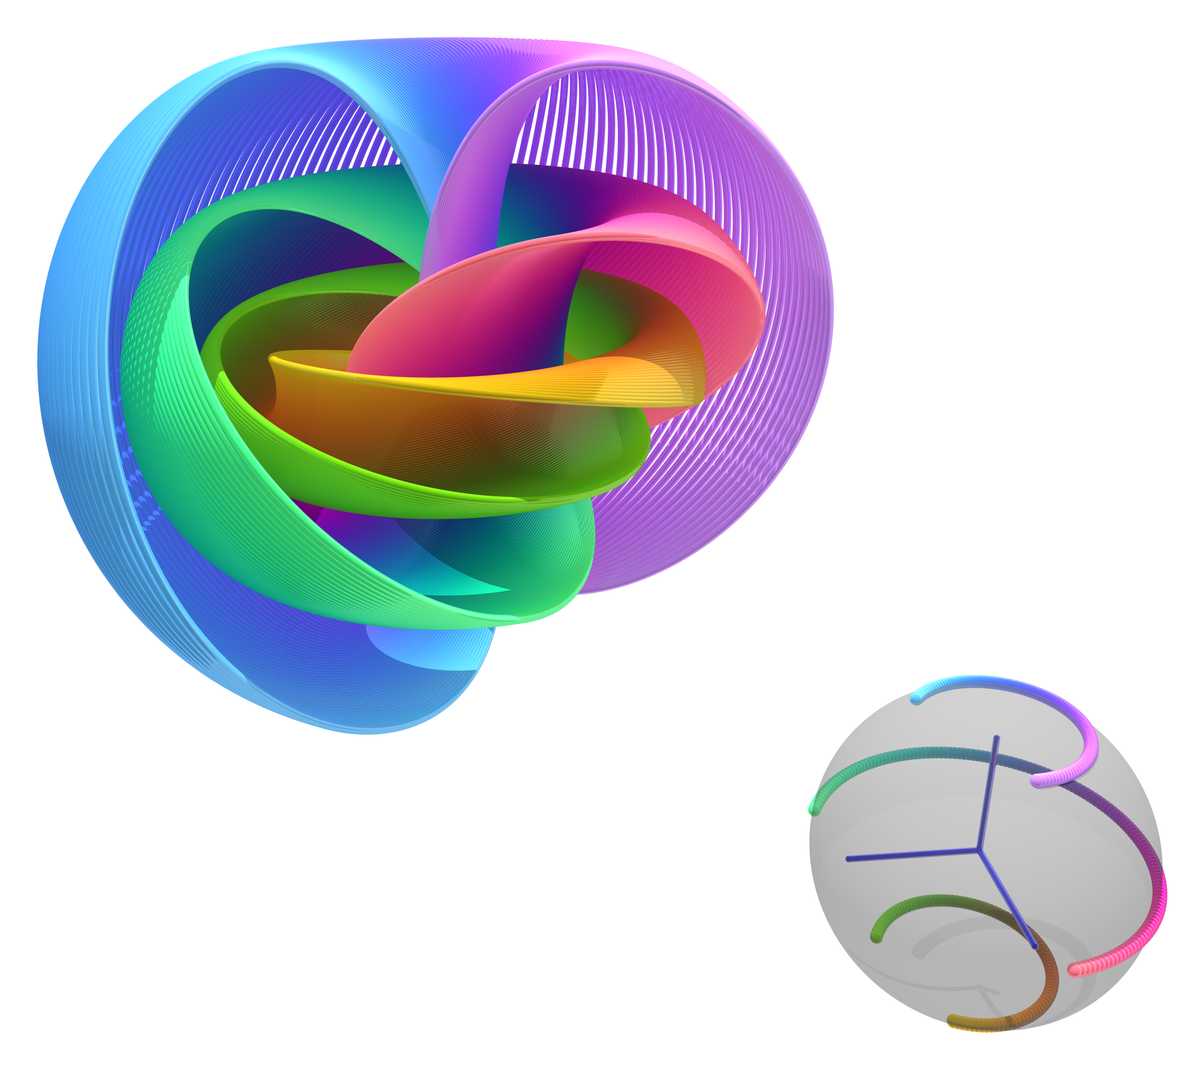
\includegraphics[height= 0.4\textheight]{figures/Hopf_Fibration.png} }
  \end{center}
\end{figure}

\end{frame}

\begin{frame}{Groupes d’homotopie}
Pour comprendre un espace $X$, on étudie certains invariants d’homotopie :
\pause
\begin{itemize}
  \item $\pi_0(X) \in \mathrm{Set}$ est l’ensemble des composantes connexes de $X$ ; il indique en combien de « morceaux » $X$ se décompose. 
    \pause
  \item Choisissons un point base $x\in X$. Soit $\mathrm{Map}_*(\mathbb{S}^1,X)\in \mathrm{Space}$ l’\textbf{espace} des lacets de $X$ basés en $x$. Ici, $\mathrm{Map}_*$ désigne l’\textbf{espace} des applications continues pointées, muni de la topologie issue des déformations continues. 
  \only<3>{


\tikzset{every picture/.style={line width=0.75pt}} %set default line width to 0.75pt        

\begin{tikzpicture}[x=0.75pt,y=0.75pt,yscale=-1,xscale=1]
%uncomment if require: \path (0,159); %set diagram left start at 0, and has height of 159

%Shape: Path Data [id:dp4540053028342088] 
\draw  [fill={rgb, 255:red, 248; green, 231; blue, 28 }  ,fill opacity=1 ] (104.5,10.2) .. controls (119.44,10.2) and (131.55,22.31) .. (131.55,37.24) .. controls (131.55,52.18) and (119.44,64.29) .. (104.5,64.29) .. controls (89.56,64.29) and (77.45,52.18) .. (77.45,37.24) .. controls (77.45,22.31) and (89.56,10.2) .. (104.5,10.2) -- cycle (97.36,37.24) .. controls (97.36,41.19) and (100.56,44.38) .. (104.5,44.38) .. controls (108.44,44.38) and (111.64,41.19) .. (111.64,37.24) .. controls (111.64,33.3) and (108.44,30.11) .. (104.5,30.11) .. controls (100.56,30.11) and (97.36,33.3) .. (97.36,37.24) -- cycle ;
%Shape: Ellipse [id:dp3307875927299506] 
\draw  [fill={rgb, 255:red, 74; green, 144; blue, 226 }  ,fill opacity=1 ] (89.47,124.4) .. controls (89.47,117.76) and (120.42,112.38) .. (158.59,112.38) .. controls (196.77,112.38) and (227.71,117.76) .. (227.71,124.4) .. controls (227.71,131.04) and (196.77,136.42) .. (158.59,136.42) .. controls (120.42,136.42) and (89.47,131.04) .. (89.47,124.4) -- cycle ;
%Curve Lines [id:da780340196334498] 
\draw    (89.17,36.04) .. controls (88.22,42.75) and (86.78,44.24) .. (90.02,50.61) .. controls (93.26,56.99) and (98.55,57.12) .. (102.59,55.1) .. controls (106.15,53.32) and (94.82,41.8) .. (90.5,37.4) ;
\draw [shift={(89.17,36.04)}, rotate = 46.78] [color={rgb, 255:red, 0; green, 0; blue, 0 }  ][line width=0.75]    (10.93,-3.29) .. controls (6.95,-1.4) and (3.31,-0.3) .. (0,0) .. controls (3.31,0.3) and (6.95,1.4) .. (10.93,3.29)   ;
%Straight Lines [id:da04091701099924694] 
\draw  [dash pattern={on 4.5pt off 4.5pt}]  (107.5,72.1) -- (107.5,110.38) ;
\draw [shift={(107.5,112.38)}, rotate = 270] [color={rgb, 255:red, 0; green, 0; blue, 0 }  ][line width=0.75]    (10.93,-3.29) .. controls (6.95,-1.4) and (3.31,-0.3) .. (0,0) .. controls (3.31,0.3) and (6.95,1.4) .. (10.93,3.29)   ;
\draw [shift={(107.5,72.1)}, rotate = 270] [color={rgb, 255:red, 0; green, 0; blue, 0 }  ][line width=0.75]    (0,5.59) -- (0,-5.59)   ;
%Shape: Ellipse [id:dp5896237309507917] 
\draw  [fill={rgb, 255:red, 0; green, 0; blue, 0 }  ,fill opacity=1 ] (104.5,123.19) .. controls (104.5,121.53) and (105.84,120.19) .. (107.5,120.19) .. controls (109.16,120.19) and (110.51,121.53) .. (110.51,123.19) .. controls (110.51,124.85) and (109.16,126.2) .. (107.5,126.2) .. controls (105.84,126.2) and (104.5,124.85) .. (104.5,123.19) -- cycle ;
%Shape: Path Data [id:dp6811427638287992] 
\draw  [fill={rgb, 255:red, 248; green, 231; blue, 28 }  ,fill opacity=1 ] (188.65,10.2) .. controls (203.58,10.2) and (215.69,22.31) .. (215.69,37.24) .. controls (215.69,52.18) and (203.58,64.29) .. (188.65,64.29) .. controls (173.71,64.29) and (161.6,52.18) .. (161.6,37.24) .. controls (161.6,22.31) and (173.71,10.2) .. (188.65,10.2) -- cycle (181.51,37.24) .. controls (181.51,41.19) and (184.7,44.38) .. (188.65,44.38) .. controls (192.59,44.38) and (195.78,41.19) .. (195.78,37.24) .. controls (195.78,33.3) and (192.59,30.11) .. (188.65,30.11) .. controls (184.7,30.11) and (181.51,33.3) .. (181.51,37.24) -- cycle ;
%Curve Lines [id:da30553399516321345] 
\draw    (173.32,36.04) .. controls (170.95,44.07) and (174.11,47.63) .. (179.63,52.27) .. controls (185.15,56.91) and (198.11,57.53) .. (203.67,52.27) .. controls (209.23,47.01) and (207.54,31.96) .. (206.89,27.16) .. controls (206.23,22.37) and (184.59,11.25) .. (179.63,16.21) .. controls (174.67,21.16) and (199.62,23.27) .. (202.72,26.14) .. controls (205.83,29.02) and (207.01,36.89) .. (203.67,40.25) .. controls (200.34,43.61) and (190,50.92) .. (185.34,48.06) .. controls (181.43,45.66) and (177.22,40.53) .. (174.62,37.51) ;
\draw [shift={(173.32,36.04)}, rotate = 46.78] [color={rgb, 255:red, 0; green, 0; blue, 0 }  ][line width=0.75]    (10.93,-3.29) .. controls (6.95,-1.4) and (3.31,-0.3) .. (0,0) .. controls (3.31,0.3) and (6.95,1.4) .. (10.93,3.29)   ;
%Straight Lines [id:da6537731025418496] 
\draw  [dash pattern={on 4.5pt off 4.5pt}]  (191.65,72.1) -- (191.65,110.38) ;
\draw [shift={(191.65,112.38)}, rotate = 270] [color={rgb, 255:red, 0; green, 0; blue, 0 }  ][line width=0.75]    (10.93,-3.29) .. controls (6.95,-1.4) and (3.31,-0.3) .. (0,0) .. controls (3.31,0.3) and (6.95,1.4) .. (10.93,3.29)   ;
\draw [shift={(191.65,72.1)}, rotate = 270] [color={rgb, 255:red, 0; green, 0; blue, 0 }  ][line width=0.75]    (0,5.59) -- (0,-5.59)   ;
%Shape: Ellipse [id:dp5922107371719822] 
\draw  [fill={rgb, 255:red, 0; green, 0; blue, 0 }  ,fill opacity=1 ] (188.65,121.39) .. controls (188.65,119.73) and (189.99,118.39) .. (191.65,118.39) .. controls (193.31,118.39) and (194.66,119.73) .. (194.66,121.39) .. controls (194.66,123.05) and (193.31,124.4) .. (191.65,124.4) .. controls (189.99,124.4) and (188.65,123.05) .. (188.65,121.39) -- cycle ;
%Shape: Path Data [id:dp8732098710208065] 
\draw  [fill={rgb, 255:red, 248; green, 231; blue, 28 }  ,fill opacity=1 ] (266.78,10.2) .. controls (281.72,10.2) and (293.83,22.31) .. (293.83,37.24) .. controls (293.83,52.18) and (281.72,64.29) .. (266.78,64.29) .. controls (251.85,64.29) and (239.74,52.18) .. (239.74,37.24) .. controls (239.74,22.31) and (251.85,10.2) .. (266.78,10.2) -- cycle (259.65,37.24) .. controls (259.65,41.19) and (262.84,44.38) .. (266.78,44.38) .. controls (270.73,44.38) and (273.92,41.19) .. (273.92,37.24) .. controls (273.92,33.3) and (270.73,30.11) .. (266.78,30.11) .. controls (262.84,30.11) and (259.65,33.3) .. (259.65,37.24) -- cycle ;
%Shape: Ellipse [id:dp7760740854975061] 
\draw  [fill={rgb, 255:red, 74; green, 144; blue, 226 }  ,fill opacity=1 ] (251.76,124.4) .. controls (251.76,117.76) and (282.7,112.38) .. (320.88,112.38) .. controls (359.05,112.38) and (390,117.76) .. (390,124.4) .. controls (390,131.04) and (359.05,136.42) .. (320.88,136.42) .. controls (282.7,136.42) and (251.76,131.04) .. (251.76,124.4) -- cycle ;
%Curve Lines [id:da9722804882352947] 
\draw    (251.46,36.04) .. controls (251.61,41) and (252.96,49.46) .. (257.77,52.27) .. controls (262.58,55.07) and (285.72,54.37) .. (287.82,40.25) .. controls (289.92,26.12) and (279,20.61) .. (269.79,22.22) .. controls (261.26,23.7) and (258.22,29.3) .. (252.82,34.73) ;
\draw [shift={(251.46,36.04)}, rotate = 317.37] [color={rgb, 255:red, 0; green, 0; blue, 0 }  ][line width=0.75]    (10.93,-3.29) .. controls (6.95,-1.4) and (3.31,-0.3) .. (0,0) .. controls (3.31,0.3) and (6.95,1.4) .. (10.93,3.29)   ;
%Straight Lines [id:da8713544464455902] 
\draw  [dash pattern={on 4.5pt off 4.5pt}]  (269.79,72.1) -- (269.79,110.38) ;
\draw [shift={(269.79,112.38)}, rotate = 270] [color={rgb, 255:red, 0; green, 0; blue, 0 }  ][line width=0.75]    (10.93,-3.29) .. controls (6.95,-1.4) and (3.31,-0.3) .. (0,0) .. controls (3.31,0.3) and (6.95,1.4) .. (10.93,3.29)   ;
\draw [shift={(269.79,72.1)}, rotate = 270] [color={rgb, 255:red, 0; green, 0; blue, 0 }  ][line width=0.75]    (0,5.59) -- (0,-5.59)   ;
%Shape: Ellipse [id:dp3298016132825492] 
\draw  [fill={rgb, 255:red, 0; green, 0; blue, 0 }  ,fill opacity=1 ] (266.78,123.19) .. controls (266.78,121.53) and (268.13,120.19) .. (269.79,120.19) .. controls (271.45,120.19) and (272.79,121.53) .. (272.79,123.19) .. controls (272.79,124.85) and (271.45,126.2) .. (269.79,126.2) .. controls (268.13,126.2) and (266.78,124.85) .. (266.78,123.19) -- cycle ;
%Shape: Path Data [id:dp29074916293433994] 
\draw  [fill={rgb, 255:red, 248; green, 231; blue, 28 }  ,fill opacity=1 ] (350.93,10.2) .. controls (365.87,10.2) and (377.98,22.31) .. (377.98,37.24) .. controls (377.98,52.18) and (365.87,64.29) .. (350.93,64.29) .. controls (335.99,64.29) and (323.88,52.18) .. (323.88,37.24) .. controls (323.88,22.31) and (335.99,10.2) .. (350.93,10.2) -- cycle (343.79,37.24) .. controls (343.79,41.19) and (346.99,44.38) .. (350.93,44.38) .. controls (354.87,44.38) and (358.07,41.19) .. (358.07,37.24) .. controls (358.07,33.3) and (354.87,30.11) .. (350.93,30.11) .. controls (346.99,30.11) and (343.79,33.3) .. (343.79,37.24) -- cycle ;
%Curve Lines [id:da4112727005454857] 
\draw    (335.6,36.04) .. controls (333.24,44.07) and (336.4,47.63) .. (341.92,52.27) .. controls (347.44,56.91) and (360.4,57.53) .. (365.96,52.27) .. controls (371.52,47.01) and (372.38,39.32) .. (369.17,27.16) .. controls (365.96,15) and (346.87,11.25) .. (341.92,16.21) .. controls (336.96,21.16) and (355.29,18.69) .. (359.95,22.22) .. controls (364.61,25.74) and (369.29,36.89) .. (365.96,40.25) .. controls (362.62,43.61) and (367.16,29.43) .. (353.94,28.23) .. controls (341.37,27.09) and (345.09,27.39) .. (336.99,34.81) ;
\draw [shift={(335.6,36.04)}, rotate = 319.02] [color={rgb, 255:red, 0; green, 0; blue, 0 }  ][line width=0.75]    (10.93,-3.29) .. controls (6.95,-1.4) and (3.31,-0.3) .. (0,0) .. controls (3.31,0.3) and (6.95,1.4) .. (10.93,3.29)   ;
%Straight Lines [id:da5705010523887033] 
\draw  [dash pattern={on 4.5pt off 4.5pt}]  (353.94,72.1) -- (353.94,110.38) ;
\draw [shift={(353.94,112.38)}, rotate = 270] [color={rgb, 255:red, 0; green, 0; blue, 0 }  ][line width=0.75]    (10.93,-3.29) .. controls (6.95,-1.4) and (3.31,-0.3) .. (0,0) .. controls (3.31,0.3) and (6.95,1.4) .. (10.93,3.29)   ;
\draw [shift={(353.94,72.1)}, rotate = 270] [color={rgb, 255:red, 0; green, 0; blue, 0 }  ][line width=0.75]    (0,5.59) -- (0,-5.59)   ;
%Shape: Ellipse [id:dp621732758556254] 
\draw  [fill={rgb, 255:red, 0; green, 0; blue, 0 }  ,fill opacity=1 ] (350.93,121.39) .. controls (350.93,119.73) and (352.28,118.39) .. (353.94,118.39) .. controls (355.6,118.39) and (356.94,119.73) .. (356.94,121.39) .. controls (356.94,123.05) and (355.6,124.4) .. (353.94,124.4) .. controls (352.28,124.4) and (350.93,123.05) .. (350.93,121.39) -- cycle ;

% Text Node
\draw (59.63,44.67) node [anchor=north west][inner sep=0.75pt]    {$X$};
% Text Node
\draw (3,95.4) node [anchor=north west][inner sep=0.75pt]    {$\mathrm{Map}_{*}\left(\mathbb{S}^{1} ,X\right)$};
% Text Node
\draw (84.97,22.43) node [anchor=north west][inner sep=0.75pt]    {$x$};
% Text Node
\draw (169.12,22.43) node [anchor=north west][inner sep=0.75pt]    {$x$};
% Text Node
\draw (131.77,26.64) node [anchor=north west][inner sep=0.75pt]    {$\cdots $};
% Text Node
\draw (243.95,21.23) node [anchor=north west][inner sep=0.75pt]    {$x$};
% Text Node
\draw (328.1,21.23) node [anchor=north west][inner sep=0.75pt]    {$x$};
% Text Node
\draw (294.06,26.64) node [anchor=north west][inner sep=0.75pt]    {$\cdots $};
% Text Node
\draw (390,112.4) node [anchor=north west][inner sep=0.75pt]    {$\cdots $};
% Text Node
\draw (61,112.4) node [anchor=north west][inner sep=0.75pt]    {$\cdots $};


\end{tikzpicture}
  }
    \pause
  \item $\pi_1(X,x) := \pi_0\mathrm{Map}_*(\mathbb{S}^1,X) \in \mathrm{Group}$ classe les lacets de $X$ à déformation près. C’est le groupe fondamental.
    \pause
  \item Pour $i>1$, $\pi_i(X,x) := \pi_0\mathrm{Map}_*(\mathbb{S}^i,X)\cong \pi_0\mathrm{Map}_*(\mathbb{S}^1,\mathrm{Map}_*(\mathbb{S}^{i-1},X)) \in \mathrm{Abel}$. C’est le $i$-ième groupe d’homotopie.
\end{itemize}
\pause
Étudions maintenant le cas $X=\mathbb{S}^n$.
\end{frame}

\begin{frame}<1-3>[label=ldm]{Groupes d’homotopie des sphères}
\begin{itemize}
  \item Pour $i<n$, on a $\pi_i(\mathbb{S}^n)=\{0\}$, où $0: \mathbb{S}^i\to * \xrightarrow{\mathrm{base}} \mathbb{S}^n$ est l’application constante.
    \pause
  \item Pour étudier $\pi_n(\mathbb{S}^n)$, considérons l’espace $\mathrm{End}_*(\mathbb{S}^n):=\mathrm{Map}_*(\mathbb{S}^n,\mathbb{S}^n)$.
\end{itemize}
\pause

Soit $f\in \mathrm{End}_*(\mathbb{S}^n)$, et choisissons un petit disque $D^n_{\epsilon}\subset \mathbb{S}^n$ loin du point base. Alors, pour $\epsilon$ suffisamment petit, la préimage $f^{-1}(D^n_{\epsilon})\subset \mathbb{S}^n-\{*\}\cong \mathbb{R}^n$ est une union disjointe de disques. Remarquons que ces disques portent des orientations $+$ ou $-$.

\only<4>{
\begin{center}
  

\tikzset{every picture/.style={line width=0.75pt}} %set default line width to 0.75pt        

\begin{tikzpicture}[x=0.75pt,y=0.75pt,yscale=-1,xscale=1]
%uncomment if require: \path (0,202); %set diagram left start at 0, and has height of 202

%Shape: Square [id:dp8905246913749407] 
\draw  [fill={rgb, 255:red, 248; green, 231; blue, 28 }  ,fill opacity=1 ] (20,30) -- (130,30) -- (130,140) -- (20,140) -- cycle ;
%Shape: Ellipse [id:dp4923647235979962] 
\draw  [fill={rgb, 255:red, 208; green, 2; blue, 27 }  ,fill opacity=1 ] (29.98,65.01) .. controls (29.98,56.72) and (36.7,50) .. (44.99,50) .. controls (53.28,50) and (60,56.72) .. (60,65.01) .. controls (60,73.3) and (53.28,80.02) .. (44.99,80.02) .. controls (36.7,80.02) and (29.98,73.3) .. (29.98,65.01) -- cycle ;

%Shape: Ellipse [id:dp34722992258516694] 
\draw  [fill={rgb, 255:red, 74; green, 144; blue, 226 }  ,fill opacity=1 ] (29.98,105.01) .. controls (29.98,96.72) and (36.7,90) .. (44.99,90) .. controls (53.28,90) and (60,96.72) .. (60,105.01) .. controls (60,113.3) and (53.28,120.02) .. (44.99,120.02) .. controls (36.7,120.02) and (29.98,113.3) .. (29.98,105.01) -- cycle ;

%Shape: Ellipse [id:dp27578992636850996] 
\draw  [fill={rgb, 255:red, 74; green, 144; blue, 226 }  ,fill opacity=1 ] (70,54.99) .. controls (70,46.7) and (76.72,39.98) .. (85.01,39.98) .. controls (93.3,39.98) and (100.02,46.7) .. (100.02,54.99) .. controls (100.02,63.28) and (93.3,70) .. (85.01,70) .. controls (76.72,70) and (70,63.28) .. (70,54.99) -- cycle ;

%Shape: Ellipse [id:dp28012353680678137] 
\draw  [fill={rgb, 255:red, 208; green, 2; blue, 27 }  ,fill opacity=1 ] (69.98,115.01) .. controls (69.98,106.72) and (76.7,100) .. (84.99,100) .. controls (93.28,100) and (100,106.72) .. (100,115.01) .. controls (100,123.3) and (93.28,130.02) .. (84.99,130.02) .. controls (76.7,130.02) and (69.98,123.3) .. (69.98,115.01) -- cycle ;

%Shape: Ellipse [id:dp720738770484213] 
\draw  [fill={rgb, 255:red, 74; green, 144; blue, 226 }  ,fill opacity=1 ] (90,84.99) .. controls (90,76.7) and (96.72,69.98) .. (105.01,69.98) .. controls (113.3,69.98) and (120.02,76.7) .. (120.02,84.99) .. controls (120.02,93.28) and (113.3,100) .. (105.01,100) .. controls (96.72,100) and (90,93.28) .. (90,84.99) -- cycle ;

%Straight Lines [id:da3463089522780478] 
\draw    (138,78.5) -- (141,78.5) .. controls (142.67,76.83) and (144.33,76.83) .. (146,78.5) .. controls (147.67,80.17) and (149.33,80.17) .. (151,78.5) .. controls (152.67,76.83) and (154.33,76.83) .. (156,78.5) .. controls (157.67,80.17) and (159.33,80.17) .. (161,78.5) .. controls (162.67,76.83) and (164.33,76.83) .. (166,78.5) -- (169,78.5) -- (172,78.5)(138,81.5) -- (141,81.5) .. controls (142.67,79.83) and (144.33,79.83) .. (146,81.5) .. controls (147.67,83.17) and (149.33,83.17) .. (151,81.5) .. controls (152.67,79.83) and (154.33,79.83) .. (156,81.5) .. controls (157.67,83.17) and (159.33,83.17) .. (161,81.5) .. controls (162.67,79.83) and (164.33,79.83) .. (166,81.5) -- (169,81.5) -- (172,81.5) ;
\draw [shift={(180,80)}, rotate = 180] [color={rgb, 255:red, 0; green, 0; blue, 0 }  ][line width=0.75]    (15.3,-4.61) .. controls (9.73,-1.96) and (4.63,-0.42) .. (0,0) .. controls (4.63,0.42) and (9.73,1.96) .. (15.3,4.61)   ;
\draw [shift={(130,80)}, rotate = 0] [color={rgb, 255:red, 0; green, 0; blue, 0 }  ][line width=0.75]    (15.3,-4.61) .. controls (9.73,-1.96) and (4.63,-0.42) .. (0,0) .. controls (4.63,0.42) and (9.73,1.96) .. (15.3,4.61)   ;
%Shape: Square [id:dp7083023491538014] 
\draw  [fill={rgb, 255:red, 248; green, 231; blue, 28 }  ,fill opacity=1 ] (180,30) -- (290,30) -- (290,140) -- (180,140) -- cycle ;
%Shape: Ellipse [id:dp5927711612585445] 
\draw  [fill={rgb, 255:red, 208; green, 2; blue, 27 }  ,fill opacity=1 ] (189.98,65.01) .. controls (189.98,56.72) and (196.7,50) .. (204.99,50) .. controls (213.28,50) and (220,56.72) .. (220,65.01) .. controls (220,73.3) and (213.28,80.02) .. (204.99,80.02) .. controls (196.7,80.02) and (189.98,73.3) .. (189.98,65.01) -- cycle ;

%Shape: Ellipse [id:dp8226989422743765] 
\draw  [fill={rgb, 255:red, 74; green, 144; blue, 226 }  ,fill opacity=1 ] (199.98,105.01) .. controls (199.98,96.72) and (206.7,90) .. (214.99,90) .. controls (223.28,90) and (230,96.72) .. (230,105.01) .. controls (230,113.3) and (223.28,120.02) .. (214.99,120.02) .. controls (206.7,120.02) and (199.98,113.3) .. (199.98,105.01) -- cycle ;

%Shape: Ellipse [id:dp29490845567419943] 
\draw  [fill={rgb, 255:red, 74; green, 144; blue, 226 }  ,fill opacity=1 ] (230,64.99) .. controls (230,56.7) and (236.72,49.98) .. (245.01,49.98) .. controls (253.3,49.98) and (260.02,56.7) .. (260.02,64.99) .. controls (260.02,73.28) and (253.3,80) .. (245.01,80) .. controls (236.72,80) and (230,73.28) .. (230,64.99) -- cycle ;

%Straight Lines [id:da08693758592549328] 
\draw    (298,78.5) -- (301,78.5) .. controls (302.67,76.83) and (304.33,76.83) .. (306,78.5) .. controls (307.67,80.17) and (309.33,80.17) .. (311,78.5) .. controls (312.67,76.83) and (314.33,76.83) .. (316,78.5) .. controls (317.67,80.17) and (319.33,80.17) .. (321,78.5) .. controls (322.67,76.83) and (324.33,76.83) .. (326,78.5) -- (329,78.5) -- (332,78.5)(298,81.5) -- (301,81.5) .. controls (302.67,79.83) and (304.33,79.83) .. (306,81.5) .. controls (307.67,83.17) and (309.33,83.17) .. (311,81.5) .. controls (312.67,79.83) and (314.33,79.83) .. (316,81.5) .. controls (317.67,83.17) and (319.33,83.17) .. (321,81.5) .. controls (322.67,79.83) and (324.33,79.83) .. (326,81.5) -- (329,81.5) -- (332,81.5) ;
\draw [shift={(340,80)}, rotate = 180] [color={rgb, 255:red, 0; green, 0; blue, 0 }  ][line width=0.75]    (15.3,-4.61) .. controls (9.73,-1.96) and (4.63,-0.42) .. (0,0) .. controls (4.63,0.42) and (9.73,1.96) .. (15.3,4.61)   ;
\draw [shift={(290,80)}, rotate = 0] [color={rgb, 255:red, 0; green, 0; blue, 0 }  ][line width=0.75]    (15.3,-4.61) .. controls (9.73,-1.96) and (4.63,-0.42) .. (0,0) .. controls (4.63,0.42) and (9.73,1.96) .. (15.3,4.61)   ;
%Shape: Square [id:dp3405215676117721] 
\draw  [fill={rgb, 255:red, 248; green, 231; blue, 28 }  ,fill opacity=1 ] (340,30) -- (450,30) -- (450,140) -- (340,140) -- cycle ;
%Shape: Ellipse [id:dp1508940159235368] 
\draw  [fill={rgb, 255:red, 74; green, 144; blue, 226 }  ,fill opacity=1 ] (380,64.99) .. controls (380,56.7) and (386.72,49.98) .. (395.01,49.98) .. controls (403.3,49.98) and (410.02,56.7) .. (410.02,64.99) .. controls (410.02,73.28) and (403.3,80) .. (395.01,80) .. controls (386.72,80) and (380,73.28) .. (380,64.99) -- cycle ;


% Text Node
\draw (77.81,106.21) node [anchor=north west][inner sep=0.75pt]    {$+$};
% Text Node
\draw (77.46,45.32) node [anchor=north west][inner sep=0.75pt]    {$-$};
% Text Node
\draw (37.44,95.34) node [anchor=north west][inner sep=0.75pt]    {$-$};
% Text Node
\draw (37.81,56.21) node [anchor=north west][inner sep=0.75pt]    {$+$};
% Text Node
\draw (97.46,75.32) node [anchor=north west][inner sep=0.75pt]    {$-$};
% Text Node
\draw (237.46,55.32) node [anchor=north west][inner sep=0.75pt]    {$-$};
% Text Node
\draw (207.44,95.34) node [anchor=north west][inner sep=0.75pt]    {$-$};
% Text Node
\draw (197.81,56.21) node [anchor=north west][inner sep=0.75pt]    {$+$};
% Text Node
\draw (387.46,55.32) node [anchor=north west][inner sep=0.75pt]    {$-$};


\end{tikzpicture}
\end{center}
}
\only<5>{
Cela donne un isomorphisme avec l'espace de configuration des disques.
\[ \mathrm{End}_*(\mathbb{S}^n) \cong \mathrm{Conf}^{fr}( \mathbb{R}^n) = \bigcup_{j,k}\mathrm{Emb}( \bigsqcup_j D^n_+ \sqcup \bigsqcup_k D^n_- , \mathbb{R}^n )
\]
Ainsi, $\pi_0 \mathrm{End}_*(\mathbb{S}^n) \cong \mathbb{Z}$, via $(j,k) \mapsto j-k$
}
\end{frame}

\begin{frame}

\begin{center}
  


\tikzset{every picture/.style={line width=0.75pt}} %set default line width to 0.75pt        

\begin{tikzpicture}[x=0.75pt,y=0.75pt,yscale=-1,xscale=1]
%uncomment if require: \path (0,153); %set diagram left start at 0, and has height of 153

%Straight Lines [id:da9147837729834951] 
\draw    (207.84,58.14) -- (388,58.14) ;
\draw [shift={(390,58.14)}, rotate = 180] [color={rgb, 255:red, 0; green, 0; blue, 0 }  ][line width=0.75]    (10.93,-3.29) .. controls (6.95,-1.4) and (3.31,-0.3) .. (0,0) .. controls (3.31,0.3) and (6.95,1.4) .. (10.93,3.29)   ;
%Shape: Circle [id:dp5777531688919217] 
\draw  [color={rgb, 255:red, 0; green, 0; blue, 0 }  ,draw opacity=1 ][line width=2.25]  (77.57,72.76) .. controls (77.57,54.65) and (92.25,39.97) .. (110.36,39.97) .. controls (128.47,39.97) and (143.15,54.65) .. (143.15,72.76) .. controls (143.15,90.87) and (128.47,105.55) .. (110.36,105.55) .. controls (92.25,105.55) and (77.57,90.87) .. (77.57,72.76) -- cycle ;
%Shape: Ellipse [id:dp9102995156755569] 
\draw  [fill={rgb, 255:red, 0; green, 0; blue, 0 }  ,fill opacity=1 ] (106.41,105.55) .. controls (106.41,103.37) and (108.18,101.6) .. (110.36,101.6) .. controls (112.54,101.6) and (114.31,103.37) .. (114.31,105.55) .. controls (114.31,107.73) and (112.54,109.49) .. (110.36,109.49) .. controls (108.18,109.49) and (106.41,107.73) .. (106.41,105.55) -- cycle ;
%Curve Lines [id:da5228835129809426] 
\draw    (110.66,118.9) .. controls (129.49,119.21) and (153.1,98.22) .. (153.2,76.36) .. controls (153.29,54.5) and (144.12,26.23) .. (104.62,27.79) .. controls (65.12,29.34) and (68.16,59.7) .. (68.16,82.47) .. controls (68.16,105.24) and (105.79,104.06) .. (98.52,118.9) .. controls (91.25,133.75) and (62.7,106.46) .. (62.09,76.4) .. controls (61.48,46.34) and (71.83,21.41) .. (110.69,21.71) .. controls (149.55,22.02) and (162.96,35.39) .. (159.27,76.36) .. controls (155.57,117.33) and (126.22,129.55) .. (98.52,131.05) .. controls (70.82,132.55) and (49.34,95.53) .. (49.94,76.4) .. controls (50.55,57.27) and (59.69,11.09) .. (104.62,9.57) .. controls (149.55,8.05) and (175.66,43.88) .. (171.41,82.43) .. controls (167.25,120.22) and (142.06,118.68) .. (112.48,118.89) ;
\draw [shift={(110.66,118.9)}, rotate = 359.43] [color={rgb, 255:red, 0; green, 0; blue, 0 }  ][line width=0.75]    (10.93,-3.29) .. controls (6.95,-1.4) and (3.31,-0.3) .. (0,0) .. controls (3.31,0.3) and (6.95,1.4) .. (10.93,3.29)   ;
\draw [shift={(143.82,100.6)}, rotate = 131.76] [color={rgb, 255:red, 0; green, 0; blue, 0 }  ][line width=0.75]    (10.93,-3.29) .. controls (6.95,-1.4) and (3.31,-0.3) .. (0,0) .. controls (3.31,0.3) and (6.95,1.4) .. (10.93,3.29)   ;
\draw [shift={(136.16,35.78)}, rotate = 40.93] [color={rgb, 255:red, 0; green, 0; blue, 0 }  ][line width=0.75]    (10.93,-3.29) .. controls (6.95,-1.4) and (3.31,-0.3) .. (0,0) .. controls (3.31,0.3) and (6.95,1.4) .. (10.93,3.29)   ;
\draw [shift={(70.47,50.44)}, rotate = 290.71] [color={rgb, 255:red, 0; green, 0; blue, 0 }  ][line width=0.75]    (10.93,-3.29) .. controls (6.95,-1.4) and (3.31,-0.3) .. (0,0) .. controls (3.31,0.3) and (6.95,1.4) .. (10.93,3.29)   ;
\draw [shift={(88.33,104.83)}, rotate = 207.7] [color={rgb, 255:red, 0; green, 0; blue, 0 }  ][line width=0.75]    (10.93,-3.29) .. controls (6.95,-1.4) and (3.31,-0.3) .. (0,0) .. controls (3.31,0.3) and (6.95,1.4) .. (10.93,3.29)   ;
\draw [shift={(69.44,102.75)}, rotate = 58.77] [color={rgb, 255:red, 0; green, 0; blue, 0 }  ][line width=0.75]    (10.93,-3.29) .. controls (6.95,-1.4) and (3.31,-0.3) .. (0,0) .. controls (3.31,0.3) and (6.95,1.4) .. (10.93,3.29)   ;
\draw [shift={(76.91,31.93)}, rotate = 134.27] [color={rgb, 255:red, 0; green, 0; blue, 0 }  ][line width=0.75]    (10.93,-3.29) .. controls (6.95,-1.4) and (3.31,-0.3) .. (0,0) .. controls (3.31,0.3) and (6.95,1.4) .. (10.93,3.29)   ;
\draw [shift={(154.96,39.51)}, rotate = 236.01] [color={rgb, 255:red, 0; green, 0; blue, 0 }  ][line width=0.75]    (10.93,-3.29) .. controls (6.95,-1.4) and (3.31,-0.3) .. (0,0) .. controls (3.31,0.3) and (6.95,1.4) .. (10.93,3.29)   ;
\draw [shift={(135.49,120.19)}, rotate = 323.14] [color={rgb, 255:red, 0; green, 0; blue, 0 }  ][line width=0.75]    (10.93,-3.29) .. controls (6.95,-1.4) and (3.31,-0.3) .. (0,0) .. controls (3.31,0.3) and (6.95,1.4) .. (10.93,3.29)   ;
\draw [shift={(61.1,107.95)}, rotate = 53.8] [color={rgb, 255:red, 0; green, 0; blue, 0 }  ][line width=0.75]    (10.93,-3.29) .. controls (6.95,-1.4) and (3.31,-0.3) .. (0,0) .. controls (3.31,0.3) and (6.95,1.4) .. (10.93,3.29)   ;
\draw [shift={(67.74,26.34)}, rotate = 128.24] [color={rgb, 255:red, 0; green, 0; blue, 0 }  ][line width=0.75]    (10.93,-3.29) .. controls (6.95,-1.4) and (3.31,-0.3) .. (0,0) .. controls (3.31,0.3) and (6.95,1.4) .. (10.93,3.29)   ;
\draw [shift={(159.44,34.76)}, rotate = 231.25] [color={rgb, 255:red, 0; green, 0; blue, 0 }  ][line width=0.75]    (10.93,-3.29) .. controls (6.95,-1.4) and (3.31,-0.3) .. (0,0) .. controls (3.31,0.3) and (6.95,1.4) .. (10.93,3.29)   ;
\draw [shift={(145.85,116.6)}, rotate = 341.86] [color={rgb, 255:red, 0; green, 0; blue, 0 }  ][line width=0.75]    (10.93,-3.29) .. controls (6.95,-1.4) and (3.31,-0.3) .. (0,0) .. controls (3.31,0.3) and (6.95,1.4) .. (10.93,3.29)   ;
%Shape: Circle [id:dp4888414439096558] 
\draw  [fill={rgb, 255:red, 0; green, 0; blue, 0 }  ,fill opacity=1 ] (106.72,118.9) .. controls (106.72,116.72) and (108.48,114.96) .. (110.66,114.96) .. controls (112.84,114.96) and (114.61,116.72) .. (114.61,118.9) .. controls (114.61,121.08) and (112.84,122.85) .. (110.66,122.85) .. controls (108.48,122.85) and (106.72,121.08) .. (106.72,118.9) -- cycle ;
%Curve Lines [id:da5649743485651755] 
\draw [color={rgb, 255:red, 208; green, 2; blue, 27 }  ,draw opacity=1 ][line width=6]    (92.48,46) .. controls (101.58,38.41) and (117.98,39.02) .. (128.91,46) ;
\draw  [color={rgb, 255:red, 0; green, 0; blue, 0 }  ,draw opacity=1 ][line width=1.5]  (104.62,33.86) -- (116.76,39.93) -- (104.62,46) ;
%Straight Lines [id:da12144641678689427] 
\draw    (68.19,15.64) -- (92.48,46) ;
%Straight Lines [id:da8252449195319262] 
\draw    (153.2,15.64) -- (128.91,46) ;
%Curve Lines [id:da15764960627001368] 
\draw [color={rgb, 255:red, 74; green, 144; blue, 226 }  ,draw opacity=1 ][line width=4.5]    (86.4,33.86) .. controls (104.62,25.66) and (117.98,26.87) .. (134.98,33.86) ;
%Curve Lines [id:da9785093166318308] 
\draw [color={rgb, 255:red, 208; green, 2; blue, 27 }  ,draw opacity=1 ][line width=4.5]    (80.33,27.79) .. controls (89.44,20.2) and (123.44,15.34) .. (141.05,27.79) ;
%Curve Lines [id:da07355354472310083] 
\draw [color={rgb, 255:red, 208; green, 2; blue, 27 }  ,draw opacity=1 ][line width=4.5]    (74.26,21.71) .. controls (98.55,-0.15) and (136.8,10.18) .. (147.12,21.71) ;
%Straight Lines [id:da7371503012271712] 
\draw [color={rgb, 255:red, 74; green, 144; blue, 226 }  ,draw opacity=1 ][line width=6]    (232.13,58.14) -- (262.49,58.14) ;
%Straight Lines [id:da0624911475429073] 
\draw [color={rgb, 255:red, 208; green, 2; blue, 27 }  ,draw opacity=1 ][line width=6]    (286.78,58.14) -- (317.14,58.14) ;
%Straight Lines [id:da9018444081119195] 
\draw [color={rgb, 255:red, 208; green, 2; blue, 27 }  ,draw opacity=1 ][line width=6]    (335.35,58.14) -- (365.71,58.14) ;
\draw  [color={rgb, 255:red, 0; green, 0; blue, 0 }  ,draw opacity=1 ][line width=1.5]  (292.85,52.07) -- (304.99,58.14) -- (292.85,64.22) ;
\draw  [color={rgb, 255:red, 0; green, 0; blue, 0 }  ,draw opacity=1 ][line width=1.5]  (341.42,52.07) -- (353.57,58.14) -- (341.42,64.22) ;
\draw  [color={rgb, 255:red, 0; green, 0; blue, 0 }  ,draw opacity=1 ][line width=1.5]  (256.42,64.22) -- (244.27,58.14) -- (256.42,52.07) ;

% Text Node
\draw (101,47.4) node [anchor=north west][inner sep=0.75pt]    {$D_{\epsilon }^{n}$};
% Text Node
\draw (265,72.4) node [anchor=north west][inner sep=0.75pt]    {$f^{-1}\left( D_{\epsilon }^{n}\right)$};
% Text Node
\draw (240.1,38.4) node [anchor=north west][inner sep=0.75pt]    {$-$};
% Text Node
\draw (296.98,38.4) node [anchor=north west][inner sep=0.75pt]    {$+$};
% Text Node
\draw (342.51,38.4) node [anchor=north west][inner sep=0.75pt]    {$+$};


\end{tikzpicture}

\pause


\begin{tikzpicture}[x=0.75pt,y=0.75pt,yscale=-1,xscale=1]
%uncomment if require: \path (0,167); %set diagram left start at 0, and has height of 167

%Straight Lines [id:da4097109424678873] 
\draw    (207.86,78.93) -- (388,78.93) ;
\draw [shift={(390,78.93)}, rotate = 180] [color={rgb, 255:red, 0; green, 0; blue, 0 }  ][line width=0.75]    (10.93,-3.29) .. controls (6.95,-1.4) and (3.31,-0.3) .. (0,0) .. controls (3.31,0.3) and (6.95,1.4) .. (10.93,3.29)   ;
%Shape: Ellipse [id:dp2037933356114996] 
\draw  [color={rgb, 255:red, 0; green, 0; blue, 0 }  ,draw opacity=1 ][line width=2.25]  (77.64,87.43) .. controls (77.64,69.32) and (92.32,54.64) .. (110.42,54.64) .. controls (128.53,54.64) and (143.21,69.32) .. (143.21,87.43) .. controls (143.21,105.54) and (128.53,120.21) .. (110.42,120.21) .. controls (92.32,120.21) and (77.64,105.54) .. (77.64,87.43) -- cycle ;
%Shape: Circle [id:dp21985344798556072] 
\draw  [fill={rgb, 255:red, 0; green, 0; blue, 0 }  ,fill opacity=1 ] (106.48,120.21) .. controls (106.48,118.03) and (108.24,116.27) .. (110.42,116.27) .. controls (112.6,116.27) and (114.37,118.03) .. (114.37,120.21) .. controls (114.37,122.39) and (112.6,124.16) .. (110.42,124.16) .. controls (108.24,124.16) and (106.48,122.39) .. (106.48,120.21) -- cycle ;
%Curve Lines [id:da05877208868362671] 
\draw    (110.73,133.57) .. controls (129.55,133.88) and (153.16,112.97) .. (153.26,91.12) .. controls (153.35,69.26) and (142.98,66.35) .. (147.18,60.76) .. controls (151.39,55.16) and (159.33,68.26) .. (159.33,91.03) .. controls (159.33,113.8) and (126.28,144.21) .. (98.58,145.71) .. controls (70.89,147.21) and (49.41,110.2) .. (50.01,91.07) .. controls (50.62,71.95) and (59.76,25.76) .. (104.68,24.25) .. controls (149.61,22.73) and (175.72,58.55) .. (171.47,97.1) .. controls (167.3,134.89) and (142.12,133.35) .. (112.54,133.56) ;
\draw [shift={(110.73,133.57)}, rotate = 359.43] [color={rgb, 255:red, 0; green, 0; blue, 0 }  ][line width=0.75]    (10.93,-3.29) .. controls (6.95,-1.4) and (3.31,-0.3) .. (0,0) .. controls (3.31,0.3) and (6.95,1.4) .. (10.93,3.29)   ;
\draw [shift={(143.88,115.32)}, rotate = 131.83] [color={rgb, 255:red, 0; green, 0; blue, 0 }  ][line width=0.75]    (10.93,-3.29) .. controls (6.95,-1.4) and (3.31,-0.3) .. (0,0) .. controls (3.31,0.3) and (6.95,1.4) .. (10.93,3.29)   ;
\draw [shift={(148.68,69.84)}, rotate = 67.32] [color={rgb, 255:red, 0; green, 0; blue, 0 }  ][line width=0.75]    (10.93,-3.29) .. controls (6.95,-1.4) and (3.31,-0.3) .. (0,0) .. controls (3.31,0.3) and (6.95,1.4) .. (10.93,3.29)   ;
\draw [shift={(158.47,78.6)}, rotate = 259.13] [color={rgb, 255:red, 0; green, 0; blue, 0 }  ][line width=0.75]    (10.93,-3.29) .. controls (6.95,-1.4) and (3.31,-0.3) .. (0,0) .. controls (3.31,0.3) and (6.95,1.4) .. (10.93,3.29)   ;
\draw [shift={(132.7,131.81)}, rotate = 321.34] [color={rgb, 255:red, 0; green, 0; blue, 0 }  ][line width=0.75]    (10.93,-3.29) .. controls (6.95,-1.4) and (3.31,-0.3) .. (0,0) .. controls (3.31,0.3) and (6.95,1.4) .. (10.93,3.29)   ;
\draw [shift={(61.17,122.62)}, rotate = 53.8] [color={rgb, 255:red, 0; green, 0; blue, 0 }  ][line width=0.75]    (10.93,-3.29) .. controls (6.95,-1.4) and (3.31,-0.3) .. (0,0) .. controls (3.31,0.3) and (6.95,1.4) .. (10.93,3.29)   ;
\draw [shift={(67.8,41.01)}, rotate = 128.24] [color={rgb, 255:red, 0; green, 0; blue, 0 }  ][line width=0.75]    (10.93,-3.29) .. controls (6.95,-1.4) and (3.31,-0.3) .. (0,0) .. controls (3.31,0.3) and (6.95,1.4) .. (10.93,3.29)   ;
\draw [shift={(159.5,49.43)}, rotate = 231.25] [color={rgb, 255:red, 0; green, 0; blue, 0 }  ][line width=0.75]    (10.93,-3.29) .. controls (6.95,-1.4) and (3.31,-0.3) .. (0,0) .. controls (3.31,0.3) and (6.95,1.4) .. (10.93,3.29)   ;
\draw [shift={(145.91,131.26)}, rotate = 341.86] [color={rgb, 255:red, 0; green, 0; blue, 0 }  ][line width=0.75]    (10.93,-3.29) .. controls (6.95,-1.4) and (3.31,-0.3) .. (0,0) .. controls (3.31,0.3) and (6.95,1.4) .. (10.93,3.29)   ;
%Shape: Ellipse [id:dp4119319162412425] 
\draw  [fill={rgb, 255:red, 0; green, 0; blue, 0 }  ,fill opacity=1 ] (106.78,133.57) .. controls (106.78,131.39) and (108.55,129.63) .. (110.73,129.63) .. controls (112.91,129.63) and (114.67,131.39) .. (114.67,133.57) .. controls (114.67,135.75) and (112.91,137.52) .. (110.73,137.52) .. controls (108.55,137.52) and (106.78,135.75) .. (106.78,133.57) -- cycle ;
%Curve Lines [id:da330753230875217] 
\draw [color={rgb, 255:red, 208; green, 2; blue, 27 }  ,draw opacity=1 ][line width=6]    (92.54,60.67) .. controls (101.65,53.08) and (118.04,53.69) .. (128.97,60.67) ;
\draw  [color={rgb, 255:red, 0; green, 0; blue, 0 }  ,draw opacity=1 ][line width=1.5]  (104.68,48.53) -- (116.83,54.6) -- (104.68,60.67) ;
%Straight Lines [id:da5299179660764051] 
\draw    (68.21,30.27) -- (92.54,60.67) ;
%Straight Lines [id:da7466964709549098] 
\draw    (153.26,30.32) -- (128.97,60.67) ;
%Curve Lines [id:da9724921884388225] 
\draw [color={rgb, 255:red, 208; green, 2; blue, 27 }  ,draw opacity=1 ][line width=4.5]    (74.33,36.39) .. controls (94.36,16.66) and (138.04,24.81) .. (147.18,36.39) ;
%Straight Lines [id:da26217806562722235] 
\draw [color={rgb, 255:red, 208; green, 2; blue, 27 }  ,draw opacity=1 ][line width=6]    (286.79,78.93) -- (317.14,78.93) ;
\draw  [color={rgb, 255:red, 0; green, 0; blue, 0 }  ,draw opacity=1 ][line width=1.5]  (292.86,72.86) -- (305,78.93) -- (292.86,85) ;
%Straight Lines [id:da5970011938083455] 
\draw [line width=0.75]    (181.5,0) .. controls (183.17,1.67) and (183.17,3.33) .. (181.5,5) .. controls (179.83,6.67) and (179.83,8.33) .. (181.5,10) .. controls (183.17,11.67) and (183.17,13.33) .. (181.5,15) .. controls (179.83,16.67) and (179.83,18.33) .. (181.5,20) .. controls (183.17,21.67) and (183.17,23.33) .. (181.5,25) -- (181.5,29) -- (181.5,32)(178.5,0) .. controls (180.17,1.67) and (180.17,3.33) .. (178.5,5) .. controls (176.83,6.67) and (176.83,8.33) .. (178.5,10) .. controls (180.17,11.67) and (180.17,13.33) .. (178.5,15) .. controls (176.83,16.67) and (176.83,18.33) .. (178.5,20) .. controls (180.17,21.67) and (180.17,23.33) .. (178.5,25) -- (178.5,29) -- (178.5,32) ;
\draw [shift={(180,40)}, rotate = 270] [color={rgb, 255:red, 0; green, 0; blue, 0 }  ][line width=0.75]    (13.12,-3.95) .. controls (8.34,-1.68) and (3.97,-0.36) .. (0,0) .. controls (3.97,0.36) and (8.34,1.68) .. (13.12,3.95)   ;

% Text Node
\draw (101,67.4) node [anchor=north west][inner sep=0.75pt]    {$D_{\epsilon }^{n}$};
% Text Node
\draw (265,92.4) node [anchor=north west][inner sep=0.75pt]    {$f^{-1}\left( D_{\epsilon }^{n}\right)$};
% Text Node
\draw (296.98,59.19) node [anchor=north west][inner sep=0.75pt]    {$+$};
% Text Node
\draw (191,11) node [anchor=north west][inner sep=0.75pt]   [align=left] {déformation};


\end{tikzpicture}

\end{center}

\end{frame}

\againframe<4->{ldm}

\begin{frame}{Groupes d’homotopie supérieurs des sphères}
  Que vaut $\pi_i(\mathbb{S}^n)$ lorsque $i>n$ ?
    \pause
\begin{itemize}
  \item Pour $i>1$, on a $\pi_i(\mathbb{S}^1)=\{0\}$.
    \pause
  \item Cependant, $\pi_3(\mathbb{S}^2)=\pi_0\mathrm{Map}_*(\mathbb{S}^3,\mathbb{S}^2) \ni H$, et $H \nsim 0$, c’est-à-dire que $H$ ne peut pas être déformée en l’application nulle.
\end{itemize}
Comment le voir ?
\pause
\[
  \mathrm{Map}_*(\mathbb{S}^{n+1},\mathbb{S}^n) \cong \mathrm{Map}_*(\mathbb{S}^1,\mathrm{End}_*(\mathbb{S}^n))\to \mathrm{Map}_*([0,1],\mathrm{End}_*(\mathbb{S}^n))
\]
Alors $H$ correspond à un chemin (autrement dit, à une homotopie) allant de $0\in \mathrm{End}_*(\mathbb{S}^2)$ à lui-même.

\end{frame}
\begin{frame}{Visualiser $H$ comme déformation}
  J’ai réalisé une animation pour visualiser cette déformation.
  \begin{figure}
    \begin{center}
      \href{https://www.youtube.com/watch?v=TnBWwh7I3aA}{ 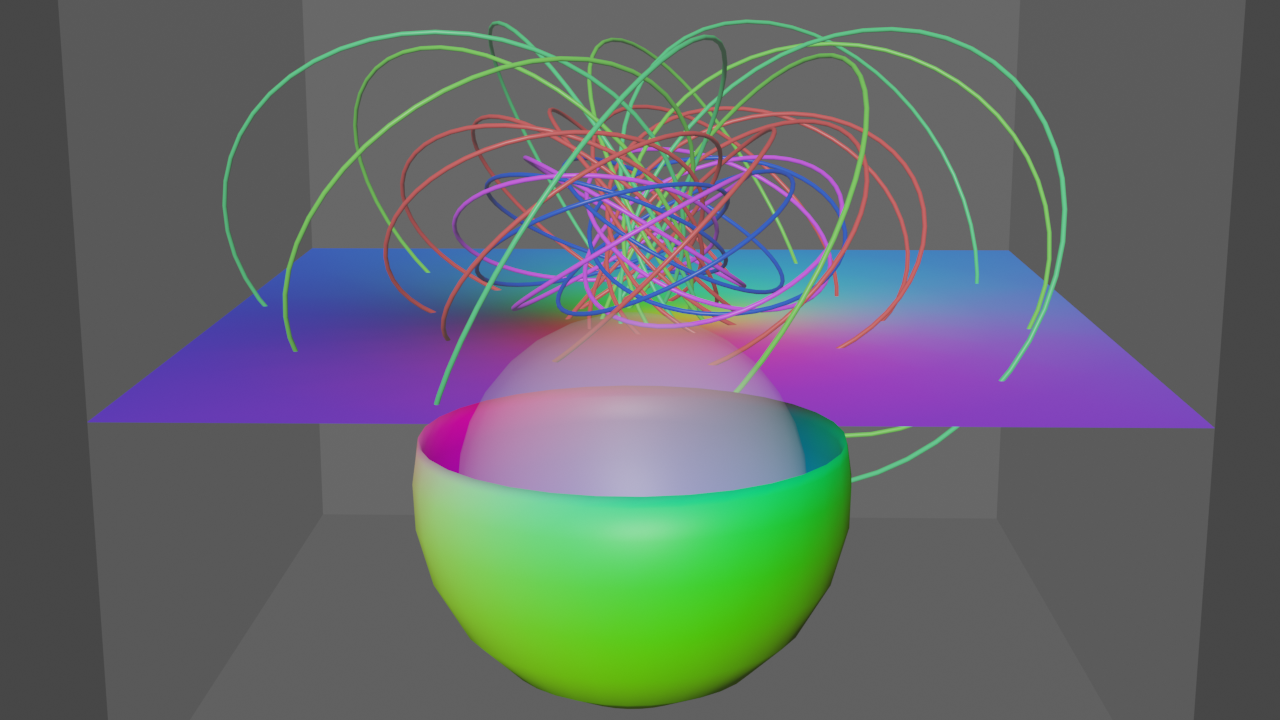
\includegraphics[height=0.3\textheight]{figures/hopf_homotopy.png} }
    \end{center}
  \end{figure}
  \pause
  On peut aussi la visualiser comme un mouvement dans l’espace de configuration ; nous y reviendrons plus tard.
 


\end{frame}
\section{Algebra}

\begin{frame}{Comment définir $\mathbb{Z}$ ?}
\pause
On peut définir les entiers naturels $\mathbb{N}$ comme les classes d’isomorphisme d’ensembles finis.
\[
  \mathrm{FinSet}_{/\cong} \xrightarrow{|\cdot|} \mathbb{N}, |X \sqcup Y| = |X|+|Y| 
\]
Comment définir les entiers relatifs $\mathbb{Z}$ à l’aide des ensembles finis ? 

\pause
On utilise le \textbf{groupe de Grothendieck} $K_0(\mathrm{FinSet})$ :
\[
  K_0(\mathrm{FinSet}) = \{ (X,Y)\in (\mathrm{FinSet}_{/\cong})^2   \} / \{ (X \sqcup Z , Y \sqcup Z) \sim (X,Y)\}
\]
On peut voir cela comme une définition formelle de $X-Y$.

\pause
Mais que vaut $K_i(\mathrm{FinSet})$ pour $i>0$ ?
\end{frame}
\begin{frame}{Espace des ensembles finis}
  Au lieu de considérer seulement l’ensemble des ensembles finis, nous considérons maintenant l’\textbf{espace (de modules)} $F = \mathrm{FinSet}^{\cong}$ : 
\begin{itemize}
  \item chaque point $x\in F$ correspond à un ensemble fini,
  \item un chemin entre deux points correspond à un isomorphisme $f:x\xrightarrow{\cong} y$ entre les ensembles finis.
\end{itemize}
  \pause

\begin{center}

\tikzset{every picture/.style={line width=0.75pt}} %set default line width to 0.75pt        

\begin{tikzpicture}[x=0.75pt,y=0.75pt,yscale=-1,xscale=1]
%uncomment if require: \path (0,157); %set diagram left start at 0, and has height of 157

%Shape: Ellipse [id:dp7720494291476914] 
\draw  [color={rgb, 255:red, 0; green, 0; blue, 0 }  ,draw opacity=1 ][fill={rgb, 255:red, 248; green, 231; blue, 28 }  ,fill opacity=1 ] (66.5,93.13) .. controls (66.5,85.88) and (74.34,80) .. (84,80) .. controls (93.66,80) and (101.5,85.88) .. (101.5,93.13) .. controls (101.5,100.37) and (93.66,106.25) .. (84,106.25) .. controls (74.34,106.25) and (66.5,100.37) .. (66.5,93.13) -- cycle ;
%Shape: Circle [id:dp8806999895439951] 
\draw  [fill={rgb, 255:red, 0; green, 0; blue, 0 }  ,fill opacity=1 ] (19,95) .. controls (19,92.24) and (21.24,90) .. (24,90) .. controls (26.76,90) and (29,92.24) .. (29,95) .. controls (29,97.76) and (26.76,100) .. (24,100) .. controls (21.24,100) and (19,97.76) .. (19,95) -- cycle ;
%Shape: Ellipse [id:dp6858466977080211] 
\draw  [color={rgb, 255:red, 0; green, 0; blue, 0 }  ,draw opacity=1 ][fill={rgb, 255:red, 248; green, 231; blue, 28 }  ,fill opacity=1 ] (129,80) .. controls (129,63.43) and (146.91,50) .. (169,50) .. controls (191.09,50) and (209,63.43) .. (209,80) .. controls (209,96.57) and (191.09,110) .. (169,110) .. controls (146.91,110) and (129,96.57) .. (129,80) -- cycle ;
%Shape: Circle [id:dp07645354210878019] 
\draw  [fill={rgb, 255:red, 0; green, 0; blue, 0 }  ,fill opacity=1 ] (79,95) .. controls (79,92.24) and (81.24,90) .. (84,90) .. controls (86.76,90) and (89,92.24) .. (89,95) .. controls (89,97.76) and (86.76,100) .. (84,100) .. controls (81.24,100) and (79,97.76) .. (79,95) -- cycle ;
%Shape: Circle [id:dp40236958016433766] 
\draw  [fill={rgb, 255:red, 0; green, 0; blue, 0 }  ,fill opacity=1 ] (159,95) .. controls (159,92.24) and (161.24,90) .. (164,90) .. controls (166.76,90) and (169,92.24) .. (169,95) .. controls (169,97.76) and (166.76,100) .. (164,100) .. controls (161.24,100) and (159,97.76) .. (159,95) -- cycle ;
%Curve Lines [id:da9320937793451245] 
\draw    (159,95) .. controls (148.85,51.44) and (201.19,51.98) .. (169.97,93.72) ;
\draw [shift={(169,95)}, rotate = 307.71] [color={rgb, 255:red, 0; green, 0; blue, 0 }  ][line width=0.75]    (10.93,-3.29) .. controls (6.95,-1.4) and (3.31,-0.3) .. (0,0) .. controls (3.31,0.3) and (6.95,1.4) .. (10.93,3.29)   ;
%Shape: Ellipse [id:dp7438442927969897] 
\draw  [color={rgb, 255:red, 0; green, 0; blue, 0 }  ,draw opacity=1 ][fill={rgb, 255:red, 248; green, 231; blue, 28 }  ,fill opacity=1 ] (219,70) .. controls (219,47.91) and (241.39,30) .. (269,30) .. controls (296.61,30) and (319,47.91) .. (319,70) .. controls (319,92.09) and (296.61,110) .. (269,110) .. controls (241.39,110) and (219,92.09) .. (219,70) -- cycle ;
%Shape: Circle [id:dp35201618999350126] 
\draw  [fill={rgb, 255:red, 0; green, 0; blue, 0 }  ,fill opacity=1 ] (259,95) .. controls (259,92.24) and (261.24,90) .. (264,90) .. controls (266.76,90) and (269,92.24) .. (269,95) .. controls (269,97.76) and (266.76,100) .. (264,100) .. controls (261.24,100) and (259,97.76) .. (259,95) -- cycle ;
%Curve Lines [id:da21588442624021154] 
\draw    (259,95) .. controls (248.85,51.44) and (301.19,51.98) .. (269.97,93.72) ;
\draw [shift={(269,95)}, rotate = 307.71] [color={rgb, 255:red, 0; green, 0; blue, 0 }  ][line width=0.75]    (10.93,-3.29) .. controls (6.95,-1.4) and (3.31,-0.3) .. (0,0) .. controls (3.31,0.3) and (6.95,1.4) .. (10.93,3.29)   ;
%Curve Lines [id:da6615814730866243] 
\draw    (259,95) .. controls (250.57,90.86) and (246.67,45) .. (279,50) .. controls (310.69,54.9) and (297.31,88.13) .. (270.65,94.64) ;
\draw [shift={(269,95)}, rotate = 348.79] [color={rgb, 255:red, 0; green, 0; blue, 0 }  ][line width=0.75]    (10.93,-3.29) .. controls (6.95,-1.4) and (3.31,-0.3) .. (0,0) .. controls (3.31,0.3) and (6.95,1.4) .. (10.93,3.29)   ;
%Curve Lines [id:da1913182351607403] 
\draw    (259,95) .. controls (236,82.33) and (227.33,29.67) .. (279,40) .. controls (329.89,50.18) and (303.49,110.81) .. (270.51,95.74) ;
\draw [shift={(269,95)}, rotate = 27.69] [color={rgb, 255:red, 0; green, 0; blue, 0 }  ][line width=0.75]    (10.93,-3.29) .. controls (6.95,-1.4) and (3.31,-0.3) .. (0,0) .. controls (3.31,0.3) and (6.95,1.4) .. (10.93,3.29)   ;

% Text Node
\draw (19,112.4) node [anchor=north west][inner sep=0.75pt]    {$\emptyset \ $};
% Text Node
\draw (60,113.4) node [anchor=north west][inner sep=0.75pt]    {$|x|=1$};
% Text Node
\draw (140,113.4) node [anchor=north west][inner sep=0.75pt]    {$|x|=\ 2$};
% Text Node
\draw (240,113.4) node [anchor=north west][inner sep=0.75pt]    {$|x|=\ 3$};
% Text Node
\draw (323,112.4) node [anchor=north west][inner sep=0.75pt]    {$\dotsc $};


\end{tikzpicture}
\end{center}
\pause
\begin{itemize}
  \item $\pi_0(F)= \mathrm{FinSet}_{/\cong} \cong \mathbb{N} $.
  \item $\pi_1(F,x) = \mathrm{S}_{|x|}$, le groupe de permutation. 
  \item $\pi_i(F,x) = \{0\}$ pour $i>1$ (On ne peut jamais déformer un isomorphisme d'un ensemble en un autre.). 

\end{itemize}
\end{frame}
\begin{frame}{K-espace (spectre) des ensembles finis}
  Nous voulons maintenant ajouter des « termes négatifs » à $F$. Pour cela, on considère l’espace $K(F)$ des \textbf{ensembles finis ordonnés} dont les éléments sont marqués par $+$ ou $-$. Nous identifions les ensembles signés ayant la même « valeur » $\|X\|=|X_+|-|X_-|$, et ces identifications sont représentées par des chemins.
\pause
\begin{center}


\tikzset{every picture/.style={line width=0.75pt}} %set default line width to 0.75pt        

\begin{tikzpicture}[x=0.75pt,y=0.75pt,yscale=-1,xscale=1]
%uncomment if require: \path (0,243); %set diagram left start at 0, and has height of 243

%Shape: Ellipse [id:dp9584335989643185] 
\draw  [color={rgb, 255:red, 0; green, 0; blue, 0 }  ,draw opacity=1 ][fill={rgb, 255:red, 208; green, 2; blue, 27 }  ,fill opacity=1 ] (219.5,134) .. controls (219.5,126.75) and (227.34,120.88) .. (237,120.88) .. controls (246.66,120.88) and (254.5,126.75) .. (254.5,134) .. controls (254.5,141.25) and (246.66,147.13) .. (237,147.13) .. controls (227.34,147.13) and (219.5,141.25) .. (219.5,134) -- cycle ;
%Shape: Circle [id:dp6840810418640495] 
\draw  [fill={rgb, 255:red, 0; green, 0; blue, 0 }  ,fill opacity=1 ] (150,135) .. controls (150,132.24) and (152.24,130) .. (155,130) .. controls (157.76,130) and (160,132.24) .. (160,135) .. controls (160,137.76) and (157.76,140) .. (155,140) .. controls (152.24,140) and (150,137.76) .. (150,135) -- cycle ;
%Shape: Ellipse [id:dp2074209970263552] 
\draw  [color={rgb, 255:red, 0; green, 0; blue, 0 }  ,draw opacity=1 ][fill={rgb, 255:red, 208; green, 2; blue, 27 }  ,fill opacity=1 ] (280,120) .. controls (280,103.43) and (297.91,90) .. (320,90) .. controls (342.09,90) and (360,103.43) .. (360,120) .. controls (360,136.57) and (342.09,150) .. (320,150) .. controls (297.91,150) and (280,136.57) .. (280,120) -- cycle ;
%Shape: Circle [id:dp075966422192562] 
\draw  [fill={rgb, 255:red, 0; green, 0; blue, 0 }  ,fill opacity=1 ] (232,134) .. controls (232,131.24) and (234.24,129) .. (237,129) .. controls (239.76,129) and (242,131.24) .. (242,134) .. controls (242,136.76) and (239.76,139) .. (237,139) .. controls (234.24,139) and (232,136.76) .. (232,134) -- cycle ;
%Shape: Circle [id:dp13601589423138405] 
\draw  [fill={rgb, 255:red, 0; green, 0; blue, 0 }  ,fill opacity=1 ] (312,134) .. controls (312,131.24) and (314.24,129) .. (317,129) .. controls (319.76,129) and (322,131.24) .. (322,134) .. controls (322,136.76) and (319.76,139) .. (317,139) .. controls (314.24,139) and (312,136.76) .. (312,134) -- cycle ;
%Curve Lines [id:da16816986849573778] 
\draw    (312,134) .. controls (301.85,90.44) and (354.19,90.98) .. (322.97,132.72) ;
\draw [shift={(322,134)}, rotate = 307.71] [color={rgb, 255:red, 0; green, 0; blue, 0 }  ][line width=0.75]    (10.93,-3.29) .. controls (6.95,-1.4) and (3.31,-0.3) .. (0,0) .. controls (3.31,0.3) and (6.95,1.4) .. (10.93,3.29)   ;
%Shape: Ellipse [id:dp22092714462956686] 
\draw  [color={rgb, 255:red, 0; green, 0; blue, 0 }  ,draw opacity=1 ][fill={rgb, 255:red, 74; green, 144; blue, 226 }  ,fill opacity=1 ] (60.44,135) .. controls (60.44,127.75) and (68.27,121.88) .. (77.94,121.88) .. controls (87.6,121.88) and (95.44,127.75) .. (95.44,135) .. controls (95.44,142.25) and (87.6,148.13) .. (77.94,148.13) .. controls (68.27,148.13) and (60.44,142.25) .. (60.44,135) -- cycle ;
%Shape: Circle [id:dp16791708812740458] 
\draw  [fill={rgb, 255:red, 0; green, 0; blue, 0 }  ,fill opacity=1 ] (72.94,135) .. controls (72.94,132.24) and (75.18,130) .. (77.94,130) .. controls (80.7,130) and (82.94,132.24) .. (82.94,135) .. controls (82.94,137.76) and (80.7,140) .. (77.94,140) .. controls (75.18,140) and (72.94,137.76) .. (72.94,135) -- cycle ;
%Shape: Ellipse [id:dp9992132530303848] 
\draw  [color={rgb, 255:red, 0; green, 0; blue, 0 }  ,draw opacity=1 ][fill={rgb, 255:red, 248; green, 231; blue, 28 }  ,fill opacity=1 ] (130,65) .. controls (130,45.67) and (141.19,30) .. (155,30) .. controls (168.81,30) and (180,45.67) .. (180,65) .. controls (180,84.33) and (168.81,100) .. (155,100) .. controls (141.19,100) and (130,84.33) .. (130,65) -- cycle ;
%Shape: Circle [id:dp2663631471602572] 
\draw  [fill={rgb, 255:red, 0; green, 0; blue, 0 }  ,fill opacity=1 ] (150,85) .. controls (150,82.24) and (152.24,80) .. (155,80) .. controls (157.76,80) and (160,82.24) .. (160,85) .. controls (160,87.76) and (157.76,90) .. (155,90) .. controls (152.24,90) and (150,87.76) .. (150,85) -- cycle ;
%Shape: Circle [id:dp9743438242870825] 
\draw  [fill={rgb, 255:red, 0; green, 0; blue, 0 }  ,fill opacity=1 ] (150,40) .. controls (150,37.24) and (152.24,35) .. (155,35) .. controls (157.76,35) and (160,37.24) .. (160,40) .. controls (160,42.76) and (157.76,45) .. (155,45) .. controls (152.24,45) and (150,42.76) .. (150,40) -- cycle ;
%Curve Lines [id:da3723191348864274] 
\draw    (155,40) .. controls (136.33,61.33) and (138.33,66.67) .. (155,85) ;
%Curve Lines [id:da7917177061632026] 
\draw    (155,85) .. controls (126.33,94.33) and (127,117.67) .. (155,135) ;
%Curve Lines [id:da48696026802363557] 
\draw    (155,40) .. controls (198.33,55.33) and (191.67,122.33) .. (155,135) ;
%Shape: Ellipse [id:dp20966307022054598] 
\draw  [color={rgb, 255:red, 0; green, 0; blue, 0 }  ,draw opacity=1 ][fill={rgb, 255:red, 248; green, 231; blue, 28 }  ,fill opacity=1 ] (52.94,66) .. controls (52.94,46.67) and (64.13,31) .. (77.94,31) .. controls (91.74,31) and (102.94,46.67) .. (102.94,66) .. controls (102.94,85.33) and (91.74,101) .. (77.94,101) .. controls (64.13,101) and (52.94,85.33) .. (52.94,66) -- cycle ;
%Shape: Circle [id:dp9073393822290099] 
\draw  [fill={rgb, 255:red, 0; green, 0; blue, 0 }  ,fill opacity=1 ] (72.94,86) .. controls (72.94,83.24) and (75.18,81) .. (77.94,81) .. controls (80.7,81) and (82.94,83.24) .. (82.94,86) .. controls (82.94,88.76) and (80.7,91) .. (77.94,91) .. controls (75.18,91) and (72.94,88.76) .. (72.94,86) -- cycle ;
%Curve Lines [id:da9045538376069651] 
\draw    (77.94,86) .. controls (50.6,101.33) and (49.94,118.67) .. (77.94,136) ;
%Curve Lines [id:da022230988628577197] 
\draw    (92.94,51) .. controls (102.6,73.33) and (95.94,82.67) .. (77.94,86) ;
%Curve Lines [id:da2903576495179958] 
\draw    (72.94,46) .. controls (50.6,70) and (61.6,75.33) .. (77.94,86) ;
%Shape: Ellipse [id:dp036971068231425264] 
\draw  [color={rgb, 255:red, 0; green, 0; blue, 0 }  ,draw opacity=1 ][fill={rgb, 255:red, 248; green, 231; blue, 28 }  ,fill opacity=1 ] (210,66) .. controls (210,46.67) and (221.19,31) .. (235,31) .. controls (248.81,31) and (260,46.67) .. (260,66) .. controls (260,85.33) and (248.81,101) .. (235,101) .. controls (221.19,101) and (210,85.33) .. (210,66) -- cycle ;
%Shape: Circle [id:dp9059746394811838] 
\draw  [fill={rgb, 255:red, 0; green, 0; blue, 0 }  ,fill opacity=1 ] (230,86) .. controls (230,83.24) and (232.24,81) .. (235,81) .. controls (237.76,81) and (240,83.24) .. (240,86) .. controls (240,88.76) and (237.76,91) .. (235,91) .. controls (232.24,91) and (230,88.76) .. (230,86) -- cycle ;
%Curve Lines [id:da2920242121207761] 
\draw    (235,86) .. controls (207.67,101.33) and (207,118.67) .. (235,136) ;
%Curve Lines [id:da5347165045324522] 
\draw    (250,51) .. controls (259.67,73.33) and (253,82.67) .. (235,86) ;
%Curve Lines [id:da09527395398351857] 
\draw    (230,46) .. controls (207.67,70) and (218.67,75.33) .. (235,86) ;
%Shape: Circle [id:dp12760776343533387] 
\draw  [fill={rgb, 255:red, 0; green, 0; blue, 0 }  ,fill opacity=1 ] (67.94,46) .. controls (67.94,43.24) and (70.18,41) .. (72.94,41) .. controls (75.7,41) and (77.94,43.24) .. (77.94,46) .. controls (77.94,48.76) and (75.7,51) .. (72.94,51) .. controls (70.18,51) and (67.94,48.76) .. (67.94,46) -- cycle ;
%Shape: Circle [id:dp02366574091579099] 
\draw  [fill={rgb, 255:red, 0; green, 0; blue, 0 }  ,fill opacity=1 ] (87.94,51) .. controls (87.94,48.24) and (90.18,46) .. (92.94,46) .. controls (95.7,46) and (97.94,48.24) .. (97.94,51) .. controls (97.94,53.76) and (95.7,56) .. (92.94,56) .. controls (90.18,56) and (87.94,53.76) .. (87.94,51) -- cycle ;
%Shape: Circle [id:dp7372981744628644] 
\draw  [fill={rgb, 255:red, 0; green, 0; blue, 0 }  ,fill opacity=1 ] (225,46) .. controls (225,43.24) and (227.24,41) .. (230,41) .. controls (232.76,41) and (235,43.24) .. (235,46) .. controls (235,48.76) and (232.76,51) .. (230,51) .. controls (227.24,51) and (225,48.76) .. (225,46) -- cycle ;
%Shape: Circle [id:dp01635578826497741] 
\draw  [fill={rgb, 255:red, 0; green, 0; blue, 0 }  ,fill opacity=1 ] (245,51) .. controls (245,48.24) and (247.24,46) .. (250,46) .. controls (252.76,46) and (255,48.24) .. (255,51) .. controls (255,53.76) and (252.76,56) .. (250,56) .. controls (247.24,56) and (245,53.76) .. (245,51) -- cycle ;
%Curve Lines [id:da368348093092131] 
\draw    (72.94,46) .. controls (86.6,34.33) and (89.27,35) .. (92.94,51) ;
%Curve Lines [id:da8538566195852573] 
\draw    (230,46) .. controls (243.67,34.33) and (246.33,35) .. (250,51) ;
%Curve Lines [id:da9826615383789019] 
\draw    (72.94,46) .. controls (13.94,66.33) and (28.6,123.67) .. (77.94,136) ;
%Curve Lines [id:da30966564066347546] 
\draw    (230,46) .. controls (215.67,42.33) and (187,126.33) .. (235,136) ;
%Curve Lines [id:da8912427859285674] 
\draw    (92.94,51) .. controls (120.6,71) and (113.94,118.33) .. (77.94,135) ;
%Curve Lines [id:da5539797399149542] 
\draw    (250,51) .. controls (293.67,71.67) and (273,133) .. (237,134) ;

% Text Node
\draw (151,143.4) node [anchor=north west][inner sep=0.75pt]    {$\emptyset \ $};
% Text Node
\draw (213,172.4) node [anchor=north west][inner sep=0.75pt]    {$\| x\| =1$};
% Text Node
\draw (293,172.4) node [anchor=north west][inner sep=0.75pt]    {$\| x\| =\ 2$};
% Text Node
\draw (364,173.4) node [anchor=north west][inner sep=0.75pt]    {$\dotsc $};
% Text Node
\draw (43.94,173.4) node [anchor=north west][inner sep=0.75pt]    {$\| x\| =-1$};
% Text Node
\draw (4,173.4) node [anchor=north west][inner sep=0.75pt]    {$\dotsc $};
% Text Node
\draw (63.94,143.4) node [anchor=north west][inner sep=0.75pt]    {$\{-\}$};
% Text Node
\draw (225,143.4) node [anchor=north west][inner sep=0.75pt]    {$\{+\}$};
% Text Node
\draw (301,143.4) node [anchor=north west][inner sep=0.75pt]    {$\{+,+\}$};
% Text Node
\draw (136,93.4) node [anchor=north west][inner sep=0.75pt]    {$\{+,-\}$};
% Text Node
\draw (136,14.4) node [anchor=north west][inner sep=0.75pt]    {$\{-,+\}$};
% Text Node
\draw (4,54.4) node [anchor=north west][inner sep=0.75pt]    {$\dotsc $};
% Text Node
\draw (301,53.4) node [anchor=north west][inner sep=0.75pt]    {$\dotsc $};
% Text Node
\draw (56.94,3.4) node [anchor=north west][inner sep=0.75pt]    {$\dotsc $};
% Text Node
\draw (40.94,94.4) node [anchor=north west][inner sep=0.75pt]    {$\{+,-,-\}$};
% Text Node
\draw (208,94.4) node [anchor=north west][inner sep=0.75pt]    {$\{+,+,-\}$};
% Text Node
\draw (221,3.4) node [anchor=north west][inner sep=0.75pt]    {$\dotsc $};
% Text Node
\draw (131,173.4) node [anchor=north west][inner sep=0.75pt]    {$\| x\| =0$};


\end{tikzpicture}
\end{center}
\end{frame}

\begin{frame}{K-groupes des ensembles finis}
  Posons $K_i(\mathrm{FinSet})=\pi_i(K(F),\emptyset)$ pour les K-groupes supérieurs. On a alors les observations suivantes :
  \pause
  \begin{itemize}
    \item $\pi_0 K(F) = \mathbb{Z}$, by $ x \mapsto \|x\|$. Cela coïncide avec $K_0(\mathrm{FinSet})$. 
      \pause
    \item On peut construire un lacet $h\in \pi_1 (K(F),\emptyset)$ en utilisant les identifications 
      \[
        h: \emptyset \sim \{+,-\} \sim \{-,+\} \sim \emptyset
      \]
      \pause
    \item En fait, $\pi_1 (K(F),\emptyset)=\mathbb{Z}/2$, et $h$ en est un générateur. Autrement dit, $h$ donne une preuve non triviale de $0=0$. 
  \end{itemize}
  \pause
  \begin{block}{Réponse}
    On peut prouver $0=0$ de manière non triviale avec $h: 0=1-1=-1+1=0$ !
  \end{block}
\end{frame}
  
\begin{frame}{K-groupes algébriques d’un corps}
  Soit $k$ un corps. On peut effectuer la même construction pour les espaces vectoriels $k$-linéaires de dimension finie. Si l’on note $V_k=\mathrm{FinVect}_k^{\cong}$, on définit les \textbf{K-groupes algébriques} de $k$ par $K_i(k)=\pi_i (K(V_k),\mathbf{0})$.

(On peut voir les ensembles finis comme des espaces vectoriels sur $\mathbb{F}_1$.)

\pause
Les K-groupes algébriques sont des invariants fondamentaux, liés à la géométrie, à la topologie, à la théorie des anneaux et à la théorie des nombres, mais ils sont notoirement difficiles à calculer.
\pause
\begin{itemize}
  \item $K_0(k)=\mathbb{Z}$
  \item $K_1(k)=k^{\times}$
  \item $K_2(k)=k^{\times}\otimes_{\mathbb{Z}} k^{\times}/ \langle x\otimes (1-x): x\in k\setminus \{0,1\} \rangle$
    \pause
  \item $K_3(k)=???$
\end{itemize}
\end{frame}
\begin{frame}{Et plus encore ?}
  Quel est le lien entre ces deux thèmes ?
  \pause
  \begin{itemize}
    \item En fait, $K_i(\mathrm{FinSet}) \cong \lim_{n\to \infty}\pi_{i+n}(\mathbb{S}^n) = \pi^s_i(\mathbb{S})$.
  \pause
\item Ainsi, $K(F)$ peut aussi être vu comme $\mathrm{Conf}^{fr}(\mathbb{R}^{\infty})$, et le lacet $h$ comme l’application de Hopf $H$ peuvent tous deux y être représentés par des mouvements.
  \end{itemize}
  \pause
  Et en fait, ils coïncident !
  \begin{center}
    

\tikzset{every picture/.style={line width=0.75pt}} %set default line width to 0.75pt        

\begin{tikzpicture}[x=0.75pt,y=0.75pt,yscale=-1,xscale=1]
%uncomment if require: \path (0,104); %set diagram left start at 0, and has height of 104

%Shape: Rectangle [id:dp6473613603306763] 
\draw  [fill={rgb, 255:red, 248; green, 231; blue, 28 }  ,fill opacity=1 ] (10,10) -- (80,10) -- (80,80) -- (10,80) -- cycle ;
%Straight Lines [id:da797601032115151] 
\draw    (80,50) -- (98,50) ;
\draw [shift={(100,50)}, rotate = 180] [color={rgb, 255:red, 0; green, 0; blue, 0 }  ][line width=0.75]    (10.93,-3.29) .. controls (6.95,-1.4) and (3.31,-0.3) .. (0,0) .. controls (3.31,0.3) and (6.95,1.4) .. (10.93,3.29)   ;
%Shape: Rectangle [id:dp6852641801099257] 
\draw  [fill={rgb, 255:red, 248; green, 231; blue, 28 }  ,fill opacity=1 ] (100,10) -- (170,10) -- (170,80) -- (100,80) -- cycle ;
%Shape: Ellipse [id:dp6711359850260148] 
\draw  [fill={rgb, 255:red, 208; green, 2; blue, 27 }  ,fill opacity=1 ] (110,40.86) .. controls (110,34.96) and (114.78,30.17) .. (120.68,30.17) .. controls (126.58,30.17) and (131.37,34.96) .. (131.37,40.86) .. controls (131.37,46.76) and (126.58,51.54) .. (120.68,51.54) .. controls (114.78,51.54) and (110,46.76) .. (110,40.86) -- cycle ;

%Shape: Ellipse [id:dp4660922965086378] 
\draw  [fill={rgb, 255:red, 74; green, 144; blue, 226 }  ,fill opacity=1 ] (140,49.32) .. controls (140,43.42) and (144.78,38.63) .. (150.68,38.63) .. controls (156.58,38.63) and (161.37,43.42) .. (161.37,49.32) .. controls (161.37,55.22) and (156.58,60) .. (150.68,60) .. controls (144.78,60) and (140,55.22) .. (140,49.32) -- cycle ;

%Straight Lines [id:da6728827873499814] 
\draw    (170,50) -- (188,50) ;
\draw [shift={(190,50)}, rotate = 180] [color={rgb, 255:red, 0; green, 0; blue, 0 }  ][line width=0.75]    (10.93,-3.29) .. controls (6.95,-1.4) and (3.31,-0.3) .. (0,0) .. controls (3.31,0.3) and (6.95,1.4) .. (10.93,3.29)   ;
%Shape: Rectangle [id:dp456247521401133] 
\draw  [fill={rgb, 255:red, 248; green, 231; blue, 28 }  ,fill opacity=1 ] (190,10) -- (260,10) -- (260,80) -- (190,80) -- cycle ;
%Shape: Ellipse [id:dp6395166789877584] 
\draw  [fill={rgb, 255:red, 208; green, 2; blue, 27 }  ,fill opacity=1 ] (210,61.47) .. controls (210,55.57) and (214.78,50.79) .. (220.68,50.79) .. controls (226.58,50.79) and (231.37,55.57) .. (231.37,61.47) .. controls (231.37,67.37) and (226.58,72.16) .. (220.68,72.16) .. controls (214.78,72.16) and (210,67.37) .. (210,61.47) -- cycle ;

%Shape: Ellipse [id:dp8450181846668086] 
\draw  [fill={rgb, 255:red, 74; green, 144; blue, 226 }  ,fill opacity=1 ] (218.63,31.47) .. controls (218.63,25.57) and (223.42,20.79) .. (229.32,20.79) .. controls (235.22,20.79) and (240,25.57) .. (240,31.47) .. controls (240,37.37) and (235.22,42.16) .. (229.32,42.16) .. controls (223.42,42.16) and (218.63,37.37) .. (218.63,31.47) -- cycle ;

%Straight Lines [id:da5749953405054897] 
\draw    (260,50) -- (278,50) ;
\draw [shift={(280,50)}, rotate = 180] [color={rgb, 255:red, 0; green, 0; blue, 0 }  ][line width=0.75]    (10.93,-3.29) .. controls (6.95,-1.4) and (3.31,-0.3) .. (0,0) .. controls (3.31,0.3) and (6.95,1.4) .. (10.93,3.29)   ;
%Shape: Rectangle [id:dp8134729787266461] 
\draw  [fill={rgb, 255:red, 248; green, 231; blue, 28 }  ,fill opacity=1 ] (280,10) -- (350,10) -- (350,80) -- (280,80) -- cycle ;
%Shape: Ellipse [id:dp5212553581587995] 
\draw  [fill={rgb, 255:red, 208; green, 2; blue, 27 }  ,fill opacity=1 ] (320,51.47) .. controls (320,45.57) and (324.78,40.79) .. (330.68,40.79) .. controls (336.58,40.79) and (341.37,45.57) .. (341.37,51.47) .. controls (341.37,57.37) and (336.58,62.16) .. (330.68,62.16) .. controls (324.78,62.16) and (320,57.37) .. (320,51.47) -- cycle ;

%Shape: Ellipse [id:dp11814790762656346] 
\draw  [fill={rgb, 255:red, 74; green, 144; blue, 226 }  ,fill opacity=1 ] (288.63,41.47) .. controls (288.63,35.57) and (293.42,30.79) .. (299.32,30.79) .. controls (305.22,30.79) and (310,35.57) .. (310,41.47) .. controls (310,47.37) and (305.22,52.16) .. (299.32,52.16) .. controls (293.42,52.16) and (288.63,47.37) .. (288.63,41.47) -- cycle ;

%Shape: Rectangle [id:dp03809290743825433] 
\draw  [fill={rgb, 255:red, 248; green, 231; blue, 28 }  ,fill opacity=1 ] (370,10) -- (440,10) -- (440,80) -- (370,80) -- cycle ;
%Straight Lines [id:da4431173323777904] 
\draw    (350,50) -- (368,50) ;
\draw [shift={(370,50)}, rotate = 180] [color={rgb, 255:red, 0; green, 0; blue, 0 }  ][line width=0.75]    (10.93,-3.29) .. controls (6.95,-1.4) and (3.31,-0.3) .. (0,0) .. controls (3.31,0.3) and (6.95,1.4) .. (10.93,3.29)   ;

% Text Node
\draw (143.58,40.24) node [anchor=north west][inner sep=0.75pt]    {$-$};
% Text Node
\draw (222.21,22.4) node [anchor=north west][inner sep=0.75pt]    {$-$};
% Text Node
\draw (213.45,52.4) node [anchor=north west][inner sep=0.75pt]    {$+$};
% Text Node
\draw (292.21,32.4) node [anchor=north west][inner sep=0.75pt]    {$-$};
% Text Node
\draw (323.45,42.4) node [anchor=north west][inner sep=0.75pt]    {$+$};
% Text Node
\draw (113.7,32.4) node [anchor=north west][inner sep=0.75pt]    {$+$};


\end{tikzpicture}
  \end{center}
  \pause
  \begin{block}{Nouvelle question}
    Peut-on trouver une interprétation géométrique des K-groupes d'un corps généraux $K_i(k)$ ?  
 \end{block} 
\end{frame}

\begin{frame}{Et le cobordisme ?}

Si l’on place ce mouvement dans l’espace de dimension $3$, on obtient un cercle :
\begin{columns}
  
\column{0.5\linewidth}
\centering
\tikzset{every picture/.style={line width=0.75pt}} %set default line width to 0.75pt        

\begin{tikzpicture}[x=0.75pt,y=0.75pt,yscale=-1,xscale=1]
%uncomment if require: \path (0,300); %set diagram left start at 0, and has height of 300

%Shape: Parallelogram [id:dp2829313780044411] 
\draw  [fill={rgb, 255:red, 248; green, 231; blue, 28 }  ,fill opacity=0.36 ] (206.42,188.2) -- (60.82,188.2) -- (123.22,250.6) -- (268.82,250.6) -- cycle ;
%Shape: Cube [id:dp7986901211428024] 
\draw   (268.82,92.4) -- (207.02,30.6) -- (62.82,30.6) -- (62.82,188.8) -- (124.62,250.6) -- (268.82,250.6) -- cycle ; \draw   (62.82,30.6) -- (124.62,92.4) -- (268.82,92.4) ; \draw   (124.62,92.4) -- (124.62,250.6) ;
%Shape: Parallelogram [id:dp5255134756222861] 
\draw  [fill={rgb, 255:red, 248; green, 231; blue, 28 }  ,fill opacity=0.36 ] (207.6,147.6) -- (62,147.6) -- (124.4,210) -- (270,210) -- cycle ;
%Shape: Ellipse [id:dp4175265135497843] 
\draw  [fill={rgb, 255:red, 208; green, 2; blue, 27 }  ,fill opacity=0.3 ] (200.7,190.68) .. controls (198.53,184.78) and (201.55,180) .. (207.46,180) .. controls (213.36,180) and (219.9,184.78) .. (222.07,190.68) .. controls (224.24,196.58) and (221.22,201.37) .. (215.32,201.37) .. controls (209.42,201.37) and (202.88,196.58) .. (200.7,190.68) -- cycle ;

%Shape: Ellipse [id:dp7754560794198566] 
\draw  [fill={rgb, 255:red, 74; green, 144; blue, 226 }  ,fill opacity=0.3 ] (127.91,180.68) .. controls (125.71,174.78) and (128.71,170) .. (134.62,170) .. controls (140.52,170) and (147.08,174.78) .. (149.28,180.68) .. controls (151.48,186.58) and (148.48,191.37) .. (142.57,191.37) .. controls (136.67,191.37) and (130.11,186.58) .. (127.91,180.68) -- cycle ;

%Shape: Parallelogram [id:dp6450713130827144] 
\draw  [fill={rgb, 255:red, 248; green, 231; blue, 28 }  ,fill opacity=0.36 ] (207.6,110) -- (62,110) -- (124.4,172.4) -- (270,172.4) -- cycle ;
%Shape: Ellipse [id:dp6943422388144511] 
\draw  [fill={rgb, 255:red, 74; green, 144; blue, 226 }  ,fill opacity=0.3 ] (157.91,120.68) .. controls (155.71,114.78) and (158.71,110) .. (164.62,110) .. controls (170.52,110) and (177.08,114.78) .. (179.28,120.68) .. controls (181.48,126.58) and (178.48,131.37) .. (172.57,131.37) .. controls (166.67,131.37) and (160.11,126.58) .. (157.91,120.68) -- cycle ;

%Shape: Ellipse [id:dp7158020602917834] 
\draw  [fill={rgb, 255:red, 208; green, 2; blue, 27 }  ,fill opacity=0.3 ] (170.7,159.32) .. controls (168.53,153.42) and (171.55,148.63) .. (177.46,148.63) .. controls (183.36,148.63) and (189.9,153.42) .. (192.07,159.32) .. controls (194.24,165.22) and (191.22,170) .. (185.32,170) .. controls (179.42,170) and (172.88,165.22) .. (170.7,159.32) -- cycle ;

%Shape: Parallelogram [id:dp6566271828309365] 
\draw  [fill={rgb, 255:red, 248; green, 231; blue, 28 }  ,fill opacity=0.36 ] (207,70) -- (60,70) -- (123,132.4) -- (270,132.4) -- cycle ;
%Shape: Ellipse [id:dp3125219871354805] 
\draw  [fill={rgb, 255:red, 208; green, 2; blue, 27 }  ,fill opacity=0.3 ] (120.92,99.32) .. controls (118.75,93.42) and (121.77,88.63) .. (127.67,88.63) .. controls (133.57,88.63) and (140.12,93.42) .. (142.29,99.32) .. controls (144.46,105.22) and (141.44,110) .. (135.54,110) .. controls (129.64,110) and (123.09,105.22) .. (120.92,99.32) -- cycle ;

%Shape: Ellipse [id:dp9355337572596321] 
\draw  [fill={rgb, 255:red, 74; green, 144; blue, 226 }  ,fill opacity=0.3 ] (187.91,99.32) .. controls (185.71,93.42) and (188.71,88.63) .. (194.62,88.63) .. controls (200.52,88.63) and (207.08,93.42) .. (209.28,99.32) .. controls (211.48,105.22) and (208.48,110) .. (202.57,110) .. controls (196.67,110) and (190.11,105.22) .. (187.91,99.32) -- cycle ;

%Shape: Parallelogram [id:dp42810300394364265] 
\draw  [fill={rgb, 255:red, 248; green, 231; blue, 28 }  ,fill opacity=0.36 ] (207.82,30) -- (62.22,30) -- (124.62,92.4) -- (270.22,92.4) -- cycle ;
%Curve Lines [id:da48854427697824443] 
\draw [color={rgb, 255:red, 74; green, 144; blue, 226 }  ,draw opacity=1 ]   (170,220) .. controls (143,218) and (139.19,207.92) .. (138.59,189.32) .. controls (137.99,170.72) and (142.81,133.68) .. (168.59,120.68) .. controls (194.38,107.68) and (183,116) .. (200.22,100) .. controls (217.43,84) and (195.4,59.2) .. (170,60) ;
%Curve Lines [id:da7957006804793516] 
\draw [color={rgb, 255:red, 208; green, 2; blue, 27 }  ,draw opacity=1 ]   (170,220) .. controls (194,219.2) and (212,214) .. (210,190) .. controls (208,166) and (203,161) .. (180,160) .. controls (157,159) and (130.65,113.35) .. (130.22,100) .. controls (129.78,86.65) and (137,57.8) .. (170,60) ;
%Straight Lines [id:da8213826161349653] 
\draw    (200,100) -- (190.89,81.79) ;
\draw [shift={(190,80)}, rotate = 63.43] [color={rgb, 255:red, 0; green, 0; blue, 0 }  ][line width=0.75]    (10.93,-3.29) .. controls (6.95,-1.4) and (3.31,-0.3) .. (0,0) .. controls (3.31,0.3) and (6.95,1.4) .. (10.93,3.29)   ;
%Straight Lines [id:da4206663217899813] 
\draw    (200,100) -- (218,100) ;
\draw [shift={(220,100)}, rotate = 180] [color={rgb, 255:red, 0; green, 0; blue, 0 }  ][line width=0.75]    (10.93,-3.29) .. controls (6.95,-1.4) and (3.31,-0.3) .. (0,0) .. controls (3.31,0.3) and (6.95,1.4) .. (10.93,3.29)   ;

%Straight Lines [id:da6829683618913758] 
\draw    (170,120) -- (160.89,101.79) ;
\draw [shift={(160,100)}, rotate = 63.43] [color={rgb, 255:red, 0; green, 0; blue, 0 }  ][line width=0.75]    (10.93,-3.29) .. controls (6.95,-1.4) and (3.31,-0.3) .. (0,0) .. controls (3.31,0.3) and (6.95,1.4) .. (10.93,3.29)   ;
%Straight Lines [id:da04181480795641934] 
\draw    (170,120) -- (188,120) ;
\draw [shift={(190,120)}, rotate = 180] [color={rgb, 255:red, 0; green, 0; blue, 0 }  ][line width=0.75]    (10.93,-3.29) .. controls (6.95,-1.4) and (3.31,-0.3) .. (0,0) .. controls (3.31,0.3) and (6.95,1.4) .. (10.93,3.29)   ;

%Straight Lines [id:da6390346330114314] 
\draw    (140,180) -- (130.89,161.79) ;
\draw [shift={(130,160)}, rotate = 63.43] [color={rgb, 255:red, 0; green, 0; blue, 0 }  ][line width=0.75]    (10.93,-3.29) .. controls (6.95,-1.4) and (3.31,-0.3) .. (0,0) .. controls (3.31,0.3) and (6.95,1.4) .. (10.93,3.29)   ;
%Straight Lines [id:da9267664003023888] 
\draw    (140,180) -- (158,180) ;
\draw [shift={(160,180)}, rotate = 180] [color={rgb, 255:red, 0; green, 0; blue, 0 }  ][line width=0.75]    (10.93,-3.29) .. controls (6.95,-1.4) and (3.31,-0.3) .. (0,0) .. controls (3.31,0.3) and (6.95,1.4) .. (10.93,3.29)   ;

%Straight Lines [id:da8683444534006999] 
\draw    (130,100) -- (120.89,81.79) ;
\draw [shift={(120,80)}, rotate = 63.43] [color={rgb, 255:red, 0; green, 0; blue, 0 }  ][line width=0.75]    (10.93,-3.29) .. controls (6.95,-1.4) and (3.31,-0.3) .. (0,0) .. controls (3.31,0.3) and (6.95,1.4) .. (10.93,3.29)   ;
%Straight Lines [id:da7147547632524447] 
\draw    (130,100) -- (112,100) ;
\draw [shift={(110,100)}, rotate = 360] [color={rgb, 255:red, 0; green, 0; blue, 0 }  ][line width=0.75]    (10.93,-3.29) .. controls (6.95,-1.4) and (3.31,-0.3) .. (0,0) .. controls (3.31,0.3) and (6.95,1.4) .. (10.93,3.29)   ;

%Straight Lines [id:da7193222744870296] 
\draw    (170,60) -- (160.89,41.79) ;
\draw [shift={(160,40)}, rotate = 63.43] [color={rgb, 255:red, 0; green, 0; blue, 0 }  ][line width=0.75]    (10.93,-3.29) .. controls (6.95,-1.4) and (3.31,-0.3) .. (0,0) .. controls (3.31,0.3) and (6.95,1.4) .. (10.93,3.29)   ;
%Straight Lines [id:da5058086459305744] 
\draw    (170,60) -- (170,42) ;
\draw [shift={(170,40)}, rotate = 90] [color={rgb, 255:red, 0; green, 0; blue, 0 }  ][line width=0.75]    (10.93,-3.29) .. controls (6.95,-1.4) and (3.31,-0.3) .. (0,0) .. controls (3.31,0.3) and (6.95,1.4) .. (10.93,3.29)   ;

%Straight Lines [id:da21485101615353686] 
\draw    (210,190) -- (200.89,171.79) ;
\draw [shift={(200,170)}, rotate = 63.43] [color={rgb, 255:red, 0; green, 0; blue, 0 }  ][line width=0.75]    (10.93,-3.29) .. controls (6.95,-1.4) and (3.31,-0.3) .. (0,0) .. controls (3.31,0.3) and (6.95,1.4) .. (10.93,3.29)   ;
%Straight Lines [id:da819887079574181] 
\draw    (210,190) -- (192,190) ;
\draw [shift={(190,190)}, rotate = 360] [color={rgb, 255:red, 0; green, 0; blue, 0 }  ][line width=0.75]    (10.93,-3.29) .. controls (6.95,-1.4) and (3.31,-0.3) .. (0,0) .. controls (3.31,0.3) and (6.95,1.4) .. (10.93,3.29)   ;

%Straight Lines [id:da907977701793039] 
\draw    (180,160) -- (170.89,141.79) ;
\draw [shift={(170,140)}, rotate = 63.43] [color={rgb, 255:red, 0; green, 0; blue, 0 }  ][line width=0.75]    (10.93,-3.29) .. controls (6.95,-1.4) and (3.31,-0.3) .. (0,0) .. controls (3.31,0.3) and (6.95,1.4) .. (10.93,3.29)   ;
%Straight Lines [id:da5019711894013863] 
\draw    (180,160) -- (162,160) ;
\draw [shift={(160,160)}, rotate = 360] [color={rgb, 255:red, 0; green, 0; blue, 0 }  ][line width=0.75]    (10.93,-3.29) .. controls (6.95,-1.4) and (3.31,-0.3) .. (0,0) .. controls (3.31,0.3) and (6.95,1.4) .. (10.93,3.29)   ;

%Straight Lines [id:da16885377224273834] 
\draw    (170,220) -- (160.89,201.79) ;
\draw [shift={(160,200)}, rotate = 63.43] [color={rgb, 255:red, 0; green, 0; blue, 0 }  ][line width=0.75]    (10.93,-3.29) .. controls (6.95,-1.4) and (3.31,-0.3) .. (0,0) .. controls (3.31,0.3) and (6.95,1.4) .. (10.93,3.29)   ;
%Straight Lines [id:da15238718584339161] 
\draw    (170,220) -- (170,202) ;
\draw [shift={(170,200)}, rotate = 90] [color={rgb, 255:red, 0; green, 0; blue, 0 }  ][line width=0.75]    (10.93,-3.29) .. controls (6.95,-1.4) and (3.31,-0.3) .. (0,0) .. controls (3.31,0.3) and (6.95,1.4) .. (10.93,3.29)   ;


% Text Node
\draw (126.92,92.4) node [anchor=north west][inner sep=0.75pt]    {$+$};
% Text Node
\draw (192.84,95.4) node [anchor=north west][inner sep=0.75pt]    {$-$};
% Text Node
\draw (162.84,115.77) node [anchor=north west][inner sep=0.75pt]    {$-$};
% Text Node
\draw (176.7,152.4) node [anchor=north west][inner sep=0.75pt]    {$+$};
% Text Node
\draw (206.7,183.77) node [anchor=north west][inner sep=0.75pt]    {$+$};
% Text Node
\draw (132.84,175.77) node [anchor=north west][inner sep=0.75pt]    {$-$};


\end{tikzpicture}



\pause
\column{0.5\linewidth}
Cela fournit un cercle framé, c’est-à-dire un plongement $\mathbb{S}^1 \hookrightarrow \mathbb{R}^n$ muni d’une \textbf{trivialisation} $\tau$ du fibré normal. On note $\Omega^{fr}_i$ le groupe des classes de cobordisme des variétés framées de dimension $i$. \pause On a aussi :

\[
  \Omega^{fr}_i \cong \pi^s_i(\mathbb{S}) 
\]

Par conséquent, ce cercle framé est non trivial et engendre $\Omega^{fr}_1$.

\end{columns}
\end{frame}
\section{Lasagna}
\begin{frame}{Skein-lasagna intrinsèque}
  Un $n$-\textbf{treefold} est un espace localement homéomorphe à $T\times \mathbb{R}^{n-1}$, où $T$ est un arbre. \pause
  Étant donnée une catégorie monoïdale symétrique $(\mathcal{C},\otimes)$, on définit une $n$-$(\mathcal{C},\otimes)$-\textbf{lasagne} comme un $n$-treefold framé $\mathcal{T}$ muni d’une stratification $\mathcal{S}$, dont les strates sont étiquetées de manière compatible avec la catégorie $\mathcal{C}$ :
  \pause
  \begin{itemize}
    \item les strates de codimension $i$ sont marquées par des $i$-morphismes (les $0$-morphismes sont les objets),
    \item aux branches du treefold, on indique la manière dont les morceaux se combinent au moyen du produit monoïdal $\otimes$.
  \end{itemize}

   \begin{center}
    


\tikzset{every picture/.style={line width=0.75pt}} %set default line width to 0.75pt        

\begin{tikzpicture}[x=0.75pt,y=0.75pt,yscale=-1,xscale=1]
%uncomment if require: \path (0,231); %set diagram left start at 0, and has height of 231

%Shape: Parallelogram [id:dp6996631170546035] 
\draw  [draw opacity=0][fill={rgb, 255:red, 126; green, 211; blue, 33 }  ,fill opacity=1 ] (360,140) -- (408.97,140) -- (420,170) -- (371.03,170) -- cycle ;
%Shape: Parallelogram [id:dp09581341430720358] 
\draw  [draw opacity=0][fill={rgb, 255:red, 144; green, 19; blue, 254 }  ,fill opacity=1 ] (381,100) -- (430,100) -- (409,140) -- (360,140) -- cycle ;
%Shape: Parallelogram [id:dp3501837238507518] 
\draw  [draw opacity=0][fill={rgb, 255:red, 208; green, 2; blue, 27 }  ,fill opacity=1 ] (360.4,140) -- (409,140) -- (357.6,170) -- (309,170) -- cycle ;
%Straight Lines [id:da25191378714933477] 
\draw [color={rgb, 255:red, 74; green, 144; blue, 226 }  ,draw opacity=1 ]   (130,120) -- (180,120) ;
%Straight Lines [id:da12977467382050778] 
\draw [color={rgb, 255:red, 208; green, 2; blue, 27 }  ,draw opacity=1 ]   (80.5,120.05) -- (130,120) ;
%Flowchart: Connector [id:dp8476595101018158] 
\draw  [fill={rgb, 255:red, 0; green, 0; blue, 0 }  ,fill opacity=1 ] (131.5,120) .. controls (131.5,119.17) and (130.83,118.5) .. (130,118.5) .. controls (129.17,118.5) and (128.5,119.17) .. (128.5,120) .. controls (128.5,120.83) and (129.17,121.5) .. (130,121.5) .. controls (130.83,121.5) and (131.5,120.83) .. (131.5,120) -- cycle ;
%Shape: Polygon [id:ds023537366445850916] 
\draw  [draw opacity=0][fill={rgb, 255:red, 208; green, 2; blue, 27 }  ,fill opacity=1 ] (230,90) -- (260,90) -- (260,120) -- (230,150) -- cycle ;
%Shape: Polygon [id:ds02842235664302828] 
\draw  [draw opacity=0][fill={rgb, 255:red, 126; green, 211; blue, 33 }  ,fill opacity=1 ] (260,90) -- (290,90) -- (290,150) -- (260,120) -- cycle ;
%Shape: Triangle [id:dp940170604210908] 
\draw  [draw opacity=0][fill={rgb, 255:red, 248; green, 231; blue, 28 }  ,fill opacity=1 ] (259.6,120) -- (290,150) -- (230,150) -- cycle ;
%Straight Lines [id:da7919368892196721] 
\draw    (260,90) -- (260,120) ;
%Straight Lines [id:da7442600311070939] 
\draw    (260,120) -- (230,150) ;
%Straight Lines [id:da8091223162735048] 
\draw    (290,150) -- (260,120) ;
%Straight Lines [id:da35128029961261864] 
\draw    (258.94,178.94) -- (263.99,173.89)(261.06,181.06) -- (266.11,176.01) ;
\draw [shift={(270,170)}, rotate = 135] [color={rgb, 255:red, 0; green, 0; blue, 0 }  ][line width=0.75]    (7.65,-3.43) .. controls (4.86,-1.61) and (2.31,-0.47) .. (0,0) .. controls (2.31,0.47) and (4.86,1.61) .. (7.65,3.43)   ;

% Text Node
\draw (124.44,94.82) node [anchor=north west][inner sep=0.75pt]    {$f$};
% Text Node
\draw (87.11,95.51) node [anchor=north west][inner sep=0.75pt]    {$A$};
% Text Node
\draw (159.78,95.29) node [anchor=north west][inner sep=0.75pt]    {$B$};
% Text Node
\draw (100.24,134.42) node [anchor=north west][inner sep=0.75pt]    {$A\ \xrightarrow{f} B$};
% Text Node
\draw (235,102.4) node [anchor=north west][inner sep=0.75pt]    {$A$};
% Text Node
\draw (271,102.4) node [anchor=north west][inner sep=0.75pt]    {$B$};
% Text Node
\draw (251,132.4) node [anchor=north west][inner sep=0.75pt]    {$C$};
% Text Node
\draw (260,92.4) node [anchor=north west][inner sep=0.75pt]    {$f$};
% Text Node
\draw (232,123.4) node [anchor=north west][inner sep=0.75pt]    {$g$};
% Text Node
\draw (277,122.4) node [anchor=north west][inner sep=0.75pt]    {$h$};
% Text Node
\draw (233,150.4) node [anchor=north west][inner sep=0.75pt]    {$A\ \xrightarrow{f} B$};
% Text Node
\draw (246.29,170.31) node [anchor=north west][inner sep=0.75pt]  [rotate=-45]  {$\xrightarrow[g]{}$};
% Text Node
\draw (256,182.4) node [anchor=north west][inner sep=0.75pt]    {$C$};
% Text Node
\draw (265.65,183.56) node [anchor=north west][inner sep=0.75pt]  [rotate=-305]  {$\xrightarrow[h]{}$};
% Text Node
\draw (351,142.4) node [anchor=north west][inner sep=0.75pt]    {$A$};
% Text Node
\draw (391,152.4) node [anchor=north west][inner sep=0.75pt]    {$B$};
% Text Node
\draw (371,112.4) node [anchor=north west][inner sep=0.75pt]    {$A\otimes B$};


\end{tikzpicture}
   \end{center} 
  \end{frame}
  \begin{frame}

  \begin{block}{Lien avec le « module de skein-lasagna »}
    
    Nous ne demandons pas d’espace ambiant $X$ dans lequel la lasagne serait plongée (ou, si l’on préfère, on peut prendre $X=\mathbb{R}^\infty$). Cela signifie que nous étudions la géométrie intrinsèque de la lasagne elle-même.
 \end{block} 
 \pause

    On peut voir une lasagne $L$ comme un diagramme de cordes de $\mathcal{C}$ dessiné sur $\mathcal{T}$ ; autrement dit, on peut écrire $L\in \int_{\mathcal{T}} (\mathcal{C},\otimes)$.
\pause
    \begin{block}{Cobordisme des lasagnes}
    
    Comme on s’y attend, on peut définir une relation de cobordisme entre $L_1$ et $L_2$ s’il existe une lasagne $W$ à bord telle que $\partial W = L_1 \sqcup -L_2$. On définit alors le $n$-ième \textbf{groupe de cobordisme}-$(\mathcal{C},\otimes)$, noté $\Omega^{\mathcal{C},\otimes}_n$, comme le groupe abélien engendré par les $n$-lasagnes modulo les relations de cobordisme.

  \end{block}

\end{frame}

\begin{frame}{Groupe de cobordisme-$(V_k,\oplus)$}
  \only<1-2>{Prenons comme exemple $\Omega^{V_k,\oplus}_n$, où $V_k=\mathrm{FinVect}^{\cong}_k$ est la sous-catégorie des espaces vectoriels de dimension finie dont les morphismes sont tous des isomorphismes.} Dans ce cas, on peut voir une lasagne comme un treefold/une variété muni(e) d’un \textbf{système local} en $k$.
  \pause
\begin{itemize}
  \item Clairement, $\Omega^{V_k,\oplus}_0\cong \mathbb{Z}$, classifié par la dimension.
  \pause

\item $\Omega^{V_k,\oplus}_1$ est engendré par les cercles $L_V(f)$ marqués par un espace vectoriel $V$ et une matrice $f\in \mathrm{GL}_V(k)$. En stabilisant par des matrices identité, on obtient un morphisme $L:\mathrm{GL}_{\infty}(k) \twoheadrightarrow \Omega^{V_k,\oplus}_1$.

\end{itemize}
  \begin{center}
    


\tikzset{every picture/.style={line width=0.75pt}} %set default line width to 0.75pt        

\begin{tikzpicture}[x=0.75pt,y=0.75pt,yscale=-1,xscale=1]
%uncomment if require: \path (0,156); %set diagram left start at 0, and has height of 156

%Shape: Arc [id:dp1665008079211352] 
\draw  [draw opacity=0][dash pattern={on 4.5pt off 4.5pt}] (184.19,96.87) .. controls (184.02,96.9) and (183.84,96.91) .. (183.67,96.91) .. controls (178.56,96.91) and (174.42,83.48) .. (174.42,66.91) .. controls (174.42,50.34) and (178.56,36.91) .. (183.67,36.91) .. controls (183.93,36.91) and (184.19,36.95) .. (184.45,37.02) -- (183.67,66.91) -- cycle ; \draw  [dash pattern={on 4.5pt off 4.5pt}] (184.19,96.87) .. controls (184.02,96.9) and (183.84,96.91) .. (183.67,96.91) .. controls (178.56,96.91) and (174.42,83.48) .. (174.42,66.91) .. controls (174.42,50.34) and (178.56,36.91) .. (183.67,36.91) .. controls (183.93,36.91) and (184.19,36.95) .. (184.45,37.02) ;  
%Shape: Circle [id:dp34434620773787505] 
\draw   (22.67,66.67) .. controls (22.67,52.86) and (33.86,41.67) .. (47.67,41.67) .. controls (61.47,41.67) and (72.67,52.86) .. (72.67,66.67) .. controls (72.67,80.47) and (61.47,91.67) .. (47.67,91.67) .. controls (33.86,91.67) and (22.67,80.47) .. (22.67,66.67) -- cycle ;
%Shape: Circle [id:dp5342684802497282] 
\draw  [fill={rgb, 255:red, 0; green, 0; blue, 0 }  ,fill opacity=1 ] (32.55,44.87) .. controls (32.55,43.36) and (33.76,42.15) .. (35.27,42.15) .. controls (36.77,42.15) and (37.99,43.36) .. (37.99,44.87) .. controls (37.99,46.37) and (36.77,47.59) .. (35.27,47.59) .. controls (33.76,47.59) and (32.55,46.37) .. (32.55,44.87) -- cycle ;
%Shape: Can [id:dp8303673337694337] 
\draw   (132.19,36.87) -- (184.19,36.87) .. controls (189.16,36.87) and (193.19,50.3) .. (193.19,66.87) .. controls (193.19,83.44) and (189.16,96.87) .. (184.19,96.87) -- (132.19,96.87) .. controls (127.22,96.87) and (123.19,83.44) .. (123.19,66.87) .. controls (123.19,50.3) and (127.22,36.87) .. (132.19,36.87) .. controls (137.16,36.87) and (141.19,50.3) .. (141.19,66.87) .. controls (141.19,83.44) and (137.16,96.87) .. (132.19,96.87) ;
%Shape: Circle [id:dp8607981738398717] 
\draw  [fill={rgb, 255:red, 0; green, 0; blue, 0 }  ,fill opacity=1 ] (44.95,41.67) .. controls (44.95,40.16) and (46.16,38.95) .. (47.67,38.95) .. controls (49.17,38.95) and (50.39,40.16) .. (50.39,41.67) .. controls (50.39,43.17) and (49.17,44.39) .. (47.67,44.39) .. controls (46.16,44.39) and (44.95,43.17) .. (44.95,41.67) -- cycle ;
%Curve Lines [id:da6568565725311016] 
\draw    (139.23,50.75) .. controls (150.27,47.83) and (166.03,53.55) .. (170.43,63.55) ;
%Curve Lines [id:da3461117691560027] 
\draw    (141.63,75.55) .. controls (151.63,76.11) and (167.23,71.31) .. (170.43,63.55) ;
%Straight Lines [id:da4929342704626295] 
\draw    (170.43,63.55) -- (193.63,63.31) ;
%Shape: Circle [id:dp6393608623461394] 
\draw  [fill={rgb, 255:red, 0; green, 0; blue, 0 }  ,fill opacity=1 ] (58.15,45.27) .. controls (58.15,43.76) and (59.36,42.55) .. (60.87,42.55) .. controls (62.37,42.55) and (63.59,43.76) .. (63.59,45.27) .. controls (63.59,46.77) and (62.37,47.99) .. (60.87,47.99) .. controls (59.36,47.99) and (58.15,46.77) .. (58.15,45.27) -- cycle ;
%Shape: Can [id:dp9029530593575552] 
\draw   (238.4,40.55) -- (277.95,40.55) .. controls (283.14,40.55) and (287.35,53.98) .. (287.35,70.55) .. controls (287.35,87.12) and (283.14,100.55) .. (277.95,100.55) -- (238.4,100.55) .. controls (233.21,100.55) and (229,87.12) .. (229,70.55) .. controls (229,53.98) and (233.21,40.55) .. (238.4,40.55) .. controls (243.59,40.55) and (247.8,53.98) .. (247.8,70.55) .. controls (247.8,87.12) and (243.59,100.55) .. (238.4,100.55) ;
%Straight Lines [id:da8838817730310911] 
\draw    (247.8,65.2) -- (288.08,65.22) ;
%Straight Lines [id:da9137768544706646] 
\draw    (279.24,40.55) -- (347.91,31.85) ;
%Straight Lines [id:da6090343245510165] 
\draw    (279.24,100.55) -- (345.08,112.13) ;
%Straight Lines [id:da07471767495563264] 
\draw  [dash pattern={on 2.25pt off 1.5pt}]  (279.24,40.55) -- (310.53,55.1) ;
%Straight Lines [id:da7591341693417983] 
\draw  [dash pattern={on 2.25pt off 1.5pt}]  (279.24,100.55) -- (309.2,88.1) ;
%Shape: Arc [id:dp07118059349492079] 
\draw  [draw opacity=0][dash pattern={on 4.5pt off 4.5pt}] (310.53,55.1) .. controls (312.72,56.31) and (314.4,63.23) .. (314.4,71.58) .. controls (314.4,80.78) and (312.36,88.25) .. (309.85,88.25) .. controls (307.33,88.25) and (305.29,80.78) .. (305.29,71.58) .. controls (305.29,62.37) and (307.33,54.91) .. (309.85,54.91) .. controls (309.93,54.91) and (310,54.92) .. (310.08,54.93) -- (309.85,71.58) -- cycle ; \draw  [dash pattern={on 4.5pt off 4.5pt}] (310.53,55.1) .. controls (312.72,56.31) and (314.4,63.23) .. (314.4,71.58) .. controls (314.4,80.78) and (312.36,88.25) .. (309.85,88.25) .. controls (307.33,88.25) and (305.29,80.78) .. (305.29,71.58) .. controls (305.29,62.37) and (307.33,54.91) .. (309.85,54.91) .. controls (309.93,54.91) and (310,54.92) .. (310.08,54.93) ;  
%Shape: Arc [id:dp9136640651819464] 
\draw  [draw opacity=0][dash pattern={on 4.5pt off 4.5pt}] (310.08,54.93) .. controls (318.98,55.28) and (326.08,62.38) .. (326.08,71.09) .. controls (326.08,80.02) and (318.62,87.26) .. (309.41,87.26) .. controls (309.23,87.26) and (309.06,87.26) .. (308.88,87.25) -- (309.41,71.09) -- cycle ; \draw  [dash pattern={on 4.5pt off 4.5pt}] (310.08,54.93) .. controls (318.98,55.28) and (326.08,62.38) .. (326.08,71.09) .. controls (326.08,80.02) and (318.62,87.26) .. (309.41,87.26) .. controls (309.23,87.26) and (309.06,87.26) .. (308.88,87.25) ;  
%Shape: Arc [id:dp2315394282297093] 
\draw  [draw opacity=0] (347.91,31.85) .. controls (355.51,33.18) and (361.53,50.7) .. (361.53,72.12) .. controls (361.53,94.4) and (355.01,112.47) .. (346.97,112.47) .. controls (346.33,112.47) and (345.7,112.35) .. (345.08,112.13) -- (346.97,72.12) -- cycle ; \draw   (347.91,31.85) .. controls (355.51,33.18) and (361.53,50.7) .. (361.53,72.12) .. controls (361.53,94.4) and (355.01,112.47) .. (346.97,112.47) .. controls (346.33,112.47) and (345.7,112.35) .. (345.08,112.13) ;  
%Straight Lines [id:da7482585057316815] 
\draw    (288.08,65.22) -- (361.4,58.4) ;
%Shape: Arc [id:dp3266026120120239] 
\draw  [draw opacity=0][dash pattern={on 4.5pt off 4.5pt}] (345.08,112.13) .. controls (338,109.39) and (332.55,92.54) .. (332.55,72.17) .. controls (332.55,49.88) and (339.07,31.82) .. (347.11,31.82) .. controls (347.54,31.82) and (347.96,31.87) .. (348.38,31.97) -- (347.11,72.17) -- cycle ; \draw  [dash pattern={on 4.5pt off 4.5pt}] (345.08,112.13) .. controls (338,109.39) and (332.55,92.54) .. (332.55,72.17) .. controls (332.55,49.88) and (339.07,31.82) .. (347.11,31.82) .. controls (347.54,31.82) and (347.96,31.87) .. (348.38,31.97) ;  
%Shape: Arc [id:dp1884790202794796] 
\draw  [draw opacity=0][dash pattern={on 4.5pt off 4.5pt}] (279.24,100.55) .. controls (279.07,100.58) and (278.9,100.6) .. (278.72,100.6) .. controls (273.62,100.6) and (269.47,87.16) .. (269.47,70.6) .. controls (269.47,54.03) and (273.62,40.6) .. (278.72,40.6) .. controls (278.99,40.6) and (279.25,40.63) .. (279.5,40.7) -- (278.72,70.6) -- cycle ; \draw  [dash pattern={on 4.5pt off 4.5pt}] (279.24,100.55) .. controls (279.07,100.58) and (278.9,100.6) .. (278.72,100.6) .. controls (273.62,100.6) and (269.47,87.16) .. (269.47,70.6) .. controls (269.47,54.03) and (273.62,40.6) .. (278.72,40.6) .. controls (278.99,40.6) and (279.25,40.63) .. (279.5,40.7) ;  

% Text Node
\draw (39.52,92) node [anchor=north west][inner sep=0.75pt]    {$V$};
% Text Node
\draw (31.92,19.4) node [anchor=north west][inner sep=0.75pt]    {$f$};
% Text Node
\draw (47.92,15.8) node [anchor=north west][inner sep=0.75pt]    {$g$};
% Text Node
\draw (126.29,43.12) node [anchor=north west][inner sep=0.75pt]    {$f$};
% Text Node
\draw (58.72,31.4) node [anchor=north west][inner sep=0.75pt]    {$\cdots $};
% Text Node
\draw (127.79,64.07) node [anchor=north west][inner sep=0.75pt]    {$g$};
% Text Node
\draw (193.79,54.07) node [anchor=north west][inner sep=0.75pt]    {$fg$};
% Text Node
\draw (230.47,48.8) node [anchor=north west][inner sep=0.75pt]  [font=\scriptsize]  {$f\oplus \mathrm{id}$};
% Text Node
\draw (246.87,83.13) node [anchor=north west][inner sep=0.75pt]  [font=\scriptsize]  {$V\oplus W$};
% Text Node
\draw (291.47,66.47) node [anchor=north west][inner sep=0.75pt]  [font=\scriptsize]  {$W$};
% Text Node
\draw (322.13,97.47) node [anchor=north west][inner sep=0.75pt]  [font=\scriptsize]  {$V$};
% Text Node
\draw (370.47,47.8) node [anchor=north west][inner sep=0.75pt]  [font=\scriptsize]  {$f$};
% Text Node
\draw (15.2,110.8) node [anchor=north west][inner sep=0.75pt]  [font=\footnotesize]  {$L_{V}( f,g,\dotsc )$};
% Text Node
\draw (104.4,108.8) node [anchor=north west][inner sep=0.75pt]  [font=\footnotesize]  {$L_{V}( f,g) \sim L_{V}( fg)$};
% Text Node
\draw (239.2,122) node [anchor=north west][inner sep=0.75pt]  [font=\footnotesize]  {$L_{V\oplus W}( f\oplus \mathrm{id}) \sim L_{V}( f)$};


\end{tikzpicture}
  \end{center}
    
  \end{frame}

\begin{frame}
 Nous avons une relation supplémentaire donnée par les surfaces : 
\begin{center}
  


\tikzset{every picture/.style={line width=0.75pt}} %set default line width to 0.75pt        

\begin{tikzpicture}[x=0.75pt,y=0.75pt,yscale=-1,xscale=1]
%uncomment if require: \path (0,204); %set diagram left start at 0, and has height of 204

%Curve Lines [id:da25839696198345463] 
\draw [color={rgb, 255:red, 208; green, 2; blue, 27 }  ,draw opacity=1 ] [dash pattern={on 4.5pt off 4.5pt}]  (131.1,152.57) .. controls (141.83,153.46) and (159.73,123.81) .. (159.38,113.54) ;
%Curve Lines [id:da7756479931504024] 
\draw [color={rgb, 255:red, 208; green, 2; blue, 27 }  ,draw opacity=1 ]   (117.97,94.1) .. controls (136.03,92.77) and (156.35,98.53) .. (159.38,113.54) ;
%Shape: Arc [id:dp2958131410181578] 
\draw  [draw opacity=0] (101.26,73.56) .. controls (117.45,68.03) and (137.51,64.76) .. (159.22,64.76) .. controls (213,64.76) and (256.6,84.82) .. (256.6,109.57) .. controls (256.6,134.32) and (213,154.38) .. (159.22,154.38) .. controls (138.42,154.38) and (119.15,151.38) .. (103.33,146.27) -- (159.22,109.57) -- cycle ; \draw   (101.26,73.56) .. controls (117.45,68.03) and (137.51,64.76) .. (159.22,64.76) .. controls (213,64.76) and (256.6,84.82) .. (256.6,109.57) .. controls (256.6,134.32) and (213,154.38) .. (159.22,154.38) .. controls (138.42,154.38) and (119.15,151.38) .. (103.33,146.27) ;  
%Shape: Arc [id:dp1241871896282788] 
\draw  [draw opacity=0] (208.69,107.97) .. controls (201.16,114.54) and (190.98,118.57) .. (179.78,118.57) .. controls (169.05,118.57) and (159.26,114.87) .. (151.84,108.79) -- (179.78,79.99) -- cycle ; \draw   (208.69,107.97) .. controls (201.16,114.54) and (190.98,118.57) .. (179.78,118.57) .. controls (169.05,118.57) and (159.26,114.87) .. (151.84,108.79) ;  
%Shape: Arc [id:dp922346472232386] 
\draw  [draw opacity=0] (162.61,111.95) .. controls (167.6,109.78) and (173.29,108.55) .. (179.33,108.55) .. controls (185.92,108.55) and (192.1,110.01) .. (197.39,112.57) -- (179.33,137.55) -- cycle ; \draw   (162.61,111.95) .. controls (167.6,109.78) and (173.29,108.55) .. (179.33,108.55) .. controls (185.92,108.55) and (192.1,110.01) .. (197.39,112.57) ;  
%Curve Lines [id:da31153544818714807] 
\draw [color={rgb, 255:red, 208; green, 2; blue, 27 }  ,draw opacity=1 ]   (111.92,139.85) .. controls (116.43,146.36) and (122.64,152.13) .. (131.1,152.57) ;
%Shape: Arc [id:dp40382863157541093] 
\draw  [draw opacity=0] (110.7,77.02) .. controls (123.53,74.09) and (139.12,72.37) .. (155.93,72.37) .. controls (199.8,72.37) and (235.35,84.08) .. (235.35,98.53) .. controls (235.35,112.99) and (199.8,124.7) .. (155.93,124.7) .. controls (142.52,124.7) and (129.89,123.61) .. (118.81,121.67) -- (155.93,98.53) -- cycle ; \draw  [color={rgb, 255:red, 126; green, 211; blue, 33 }  ,draw opacity=1 ] (110.7,77.02) .. controls (123.53,74.09) and (139.12,72.37) .. (155.93,72.37) .. controls (199.8,72.37) and (235.35,84.08) .. (235.35,98.53) .. controls (235.35,112.99) and (199.8,124.7) .. (155.93,124.7) .. controls (142.52,124.7) and (129.89,123.61) .. (118.81,121.67) ;  
%Shape: Ellipse [id:dp34003597646174155] 
\draw   (83.55,109.86) .. controls (83.55,90.03) and (91.73,73.95) .. (101.81,73.95) .. controls (111.9,73.95) and (120.07,90.03) .. (120.07,109.86) .. controls (120.07,129.69) and (111.9,145.77) .. (101.81,145.77) .. controls (91.73,145.77) and (83.55,129.69) .. (83.55,109.86) -- cycle ;

% Text Node
\draw (96.41,77.3) node [anchor=north west][inner sep=0.75pt]  [font=\footnotesize]  {$f$};
% Text Node
\draw (104.88,89.72) node [anchor=north west][inner sep=0.75pt]  [font=\footnotesize]  {$g$};
% Text Node
\draw (97.98,110.3) node [anchor=north west][inner sep=0.75pt]  [font=\footnotesize]  {$f^{-1}$};
% Text Node
\draw (92.41,127.58) node [anchor=north west][inner sep=0.75pt]  [font=\footnotesize]  {$g^{-1}$};
% Text Node
\draw (127,168.8) node [anchor=north west][inner sep=0.75pt]    {$L([ f,g]) \sim 0$};


\end{tikzpicture}
\end{center}
\pause
Remarquons que $k^{\times}\cong \mathrm{GL}_{\infty}(k)/[\mathrm{GL}_{\infty}(k),\mathrm{GL}_{\infty}(k)]$. En fait, on peut montrer que le morphisme induit $L:k^{\times} \xrightarrow{\cong} \Omega^{V_k,\oplus}_1$ est un isomorphisme. 

\pause
Par exemple, la lasagne induite par l’application de Hopf $H$ est alors donnée par $L(-1)$.

\end{frame}
\begin{frame}{Isomorphisme de Pontryagin--Thom généralisé}
  
Rappelons que $K_0(k)=\mathbb{Z}$ et $K_1(k)=k^{\times}$. Ce n’est pas une simple coïncidence :
\pause
\begin{block}{Isomorphisme de Pontryagin--Thom généralisé (travail en cours)}

  Pour tout $n\geq 0$, on a un isomorphisme
  \[
    K_n(k) \xrightarrow{\cong} \Omega^{V_k,\oplus}_n
  \]
  
\end{block}
\pause
Cela répond à la nouvelle question : on peut voir les lasagnes comme des éléments de K-groupes, ce qui fournit un pont entre des problèmes difficiles d’algèbre et des problèmes difficiles de topologie géométrique.

\pause
Que nous dit alors cette histoire dans le cas $n=2$ ?

\end{frame}
\begin{frame}{$\Omega^{V_k,\oplus}_2$ et $K_2(k)$}

  Pour des matrices $f,g\in \mathrm{GL}(k)$ telles que $[f,g]=1$, on peut définir la $2$-lasagne suivante $C(f,g)$ :

 \begin{center}
  


\tikzset{every picture/.style={line width=0.75pt}} %set default line width to 0.75pt        

\begin{tikzpicture}[x=0.75pt,y=0.75pt,yscale=-1,xscale=1]
%uncomment if require: \path (0,300); %set diagram left start at 0, and has height of 300

%Shape: Arc [id:dp08875951055434284] 
\draw  [draw opacity=0] (199.81,157.95) .. controls (193.54,166.8) and (184.07,172.43) .. (173.48,172.43) .. controls (163.27,172.43) and (154.1,167.19) .. (147.84,158.89) -- (173.48,132.46) -- cycle ; \draw   (199.81,157.95) .. controls (193.54,166.8) and (184.07,172.43) .. (173.48,172.43) .. controls (163.27,172.43) and (154.1,167.19) .. (147.84,158.89) ;  
%Shape: Arc [id:dp37364731845395227] 
\draw  [draw opacity=0] (156.87,167.22) .. controls (161.5,163.95) and (167.09,162.05) .. (173.11,162.05) .. controls (179.63,162.05) and (185.64,164.29) .. (190.48,168.06) -- (173.11,192.09) -- cycle ; \draw   (156.87,167.22) .. controls (161.5,163.95) and (167.09,162.05) .. (173.11,162.05) .. controls (179.63,162.05) and (185.64,164.29) .. (190.48,168.06) ;  
%Shape: Ellipse [id:dp23902327909274745] 
\draw   (93.42,166.15) .. controls (93.42,140.39) and (128.39,119.52) .. (171.52,119.52) .. controls (214.66,119.52) and (249.62,140.39) .. (249.62,166.15) .. controls (249.62,191.9) and (214.66,212.78) .. (171.52,212.78) .. controls (128.39,212.78) and (93.42,191.9) .. (93.42,166.15) -- cycle ;
%Shape: Ellipse [id:dp08445288748513025] 
\draw  [color={rgb, 255:red, 184; green, 233; blue, 134 }  ,draw opacity=1 ] (114.43,161.76) .. controls (114.43,147.23) and (140.45,135.46) .. (172.55,135.46) .. controls (204.65,135.46) and (230.66,147.23) .. (230.66,161.76) .. controls (230.66,176.28) and (204.65,188.06) .. (172.55,188.06) .. controls (140.45,188.06) and (114.43,176.28) .. (114.43,161.76) -- cycle ;
%Shape: Arc [id:dp6523650578304243] 
\draw  [draw opacity=0] (152.3,209.95) .. controls (146.23,208.2) and (141.61,199.29) .. (141.61,188.55) .. controls (141.61,176.56) and (147.37,166.84) .. (154.47,166.84) .. controls (155.29,166.84) and (156.1,166.97) .. (156.87,167.22) -- (154.47,188.55) -- cycle ; \draw  [color={rgb, 255:red, 208; green, 2; blue, 27 }  ,draw opacity=1 ] (152.3,209.95) .. controls (146.23,208.2) and (141.61,199.29) .. (141.61,188.55) .. controls (141.61,176.56) and (147.37,166.84) .. (154.47,166.84) .. controls (155.29,166.84) and (156.1,166.97) .. (156.87,167.22) ;  
%Shape: Arc [id:dp03657090661410978] 
\draw  [draw opacity=0][dash pattern={on 4.5pt off 4.5pt}] (163.47,173.03) .. controls (165.86,176.97) and (167.34,182.47) .. (167.34,188.55) .. controls (167.34,199.71) and (162.35,208.9) .. (155.93,210.12) -- (154.47,188.55) -- cycle ; \draw  [color={rgb, 255:red, 208; green, 2; blue, 27 }  ,draw opacity=1 ][dash pattern={on 4.5pt off 4.5pt}] (163.47,173.03) .. controls (165.86,176.97) and (167.34,182.47) .. (167.34,188.55) .. controls (167.34,199.71) and (162.35,208.9) .. (155.93,210.12) ;  
%Curve Lines [id:da7785889566235382] 
\draw    (155.57,193.65) .. controls (194.23,221.39) and (241.59,210.71) .. (283.69,183.6) ;
\draw [shift={(284.97,182.78)}, rotate = 146.84] [color={rgb, 255:red, 0; green, 0; blue, 0 }  ][line width=0.75]    (10.93,-3.29) .. controls (6.95,-1.4) and (3.31,-0.3) .. (0,0) .. controls (3.31,0.3) and (6.95,1.4) .. (10.93,3.29)   ;
%Straight Lines [id:da3530716693077939] 
\draw    (295.44,149.7) -- (296.29,175.27) ;
\draw [shift={(296.36,177.26)}, rotate = 268.09] [color={rgb, 255:red, 0; green, 0; blue, 0 }  ][line width=0.75]    (4.37,-1.96) .. controls (2.78,-0.92) and (1.32,-0.27) .. (0,0) .. controls (1.32,0.27) and (2.78,0.92) .. (4.37,1.96)   ;
%Straight Lines [id:da24373915684523606] 
\draw    (350.57,149.7) -- (350.57,175.26) ;
\draw [shift={(350.57,177.26)}, rotate = 270] [color={rgb, 255:red, 0; green, 0; blue, 0 }  ][line width=0.75]    (4.37,-1.96) .. controls (2.78,-0.92) and (1.32,-0.27) .. (0,0) .. controls (1.32,0.27) and (2.78,0.92) .. (4.37,1.96)   ;
%Straight Lines [id:da5911987331662195] 
\draw    (309.22,191.05) -- (334.79,191.05) ;
\draw [shift={(336.79,191.05)}, rotate = 180] [color={rgb, 255:red, 0; green, 0; blue, 0 }  ][line width=0.75]    (4.37,-1.96) .. controls (2.78,-0.92) and (1.32,-0.27) .. (0,0) .. controls (1.32,0.27) and (2.78,0.92) .. (4.37,1.96)   ;
%Straight Lines [id:da39984972337631364] 
\draw    (309.22,135.92) -- (334.79,135.92) ;
\draw [shift={(336.79,135.92)}, rotate = 180] [color={rgb, 255:red, 0; green, 0; blue, 0 }  ][line width=0.75]    (4.37,-1.96) .. controls (2.78,-0.92) and (1.32,-0.27) .. (0,0) .. controls (1.32,0.27) and (2.78,0.92) .. (4.37,1.96)   ;
%Straight Lines [id:da48473603554916134] 
\draw    (330.1,156.66) -- (316.32,172.28)(327.85,154.68) -- (314.07,170.3) ;
%Shape: Ellipse [id:dp9510867881111674] 
\draw  [dash pattern={on 0.84pt off 2.51pt}] (128.83,183.93) .. controls (128.83,175.85) and (135.38,169.3) .. (143.45,169.3) .. controls (151.53,169.3) and (158.08,175.85) .. (158.08,183.93) .. controls (158.08,192) and (151.53,198.55) .. (143.45,198.55) .. controls (135.38,198.55) and (128.83,192) .. (128.83,183.93) -- cycle ;

% Text Node
\draw (103.39,149.45) node [anchor=north west][inner sep=0.75pt]  [font=\normalsize]  {$f$};
% Text Node
\draw (134.32,209.89) node [anchor=north west][inner sep=0.75pt]  [font=\normalsize]  {$g$};
% Text Node
\draw (316.67,117.11) node [anchor=north west][inner sep=0.75pt]  [font=\small]  {$f$};
% Text Node
\draw (315.51,193.37) node [anchor=north west][inner sep=0.75pt]  [font=\small]  {$f$};
% Text Node
\draw (290.42,131.65) node [anchor=north west][inner sep=0.75pt]  [font=\small]  {$V$};
% Text Node
\draw (342.18,130.43) node [anchor=north west][inner sep=0.75pt]  [font=\small]  {$V$};
% Text Node
\draw (291.34,184.95) node [anchor=north west][inner sep=0.75pt]  [font=\small]  {$V$};
% Text Node
\draw (344.33,186.78) node [anchor=north west][inner sep=0.75pt]  [font=\small]  {$V$};
% Text Node
\draw (280.38,154.69) node [anchor=north west][inner sep=0.75pt]  [font=\small]  {$g$};
% Text Node
\draw (357.25,155.91) node [anchor=north west][inner sep=0.75pt]  [font=\small]  {$g$};
% Text Node
\draw (37,172.4) node [anchor=north west][inner sep=0.75pt]    {$C( f,g)$};


\end{tikzpicture}
 \end{center} 
 
 \pause
Rappelons que $K_2(k)= k^\times \otimes k^\times / \langle a \otimes 1-a \rangle$, ce qui signifie qu'il nous faut trouver une $3$-lasagne appelée lasagne de Ghys qui borde $C(a,1-a)$. Autrement dit, on peut encoder une preuve/un calcul par une lasagne.

\pause

Je ne dispose pas de la lasagne de Ghys pour l'instant (son genre de Heegaard est inférieur à 26), mais j'ai un exemple plus simple.
\end{frame}
\begin{frame}{Une $3$-lasagne bordes $C(e_{12}(a),e_{12}(b))$}
  \only<1-2>{ Pour $i\neq j$, définissons les matrices élémentaires $e_{ij}(a)$ par
  \[
    (e_{ij}(a))_{kl}=\begin{cases}
      1, &\text{ si }k=l,\\
      a, &\text{ si }k=i, l=j,\\
      0, &\text{ sinon.}
    \end{cases}
\]}
  \pause
  Remarquons que $e_{ij}(a)^{-1}=e_{ij}(-a)$, et qu’elles satisfont les relations de Steinberg :
  \[
    [e_{ij}(a),e_{kl}(b)]=\begin{cases}
      e_{il}(ab), &\text{ si } j=k,\\
      \mathbf{1}, &\text{ sinon. }\\
    \end{cases}
  \]
  \pause
  En utilisant ces relations et l’identité de Hall--Witt, on obtient la preuve non triviale suivante de $[e_{12}(a),e_{12}(b)]=\mathbf{1}$ :
  {\begin{eqnarray*}
    &[e_{12}(a),e_{12}(b)]=[[e_{13}(a),e_{32}(1)],e_{12}(b)]\\
    &=[e_{32}(1),[e_{13}(-a),e_{12}(-b)]]^{e_{13}(a)}[e_{13}(a),[e_{32}(-1),e_{12}(-b)]]^{e_{32}(-1)}\\
    &=[e_{32}(1),\mathbf{1}]^{e_{13}(a)}[e_{13}(a),\mathbf{1}]^{e_{32}(-1)}=\mathbf{1} 
  \end{eqnarray*}}
\end{frame}
\begin{frame}
  En suivant ce schéma, on obtient le découpage de Heegaard suivant pour construire une lasagne : 
\begin{center}


\tikzset{every picture/.style={line width=0.75pt}} %set default line width to 0.75pt        

\begin{tikzpicture}[x=0.75pt,y=0.75pt,yscale=-1,xscale=1]
%uncomment if require: \path (0,300); %set diagram left start at 0, and has height of 300

%Shape: Circle [id:dp33382124869121443] 
\draw  [fill={rgb, 255:red, 248; green, 231; blue, 28 }  ,fill opacity=1 ] (462.2,228.68) .. controls (423.94,250.77) and (375.01,237.66) .. (352.92,199.4) .. controls (330.83,161.14) and (343.94,112.21) .. (382.2,90.12) .. controls (420.46,68.03) and (469.39,81.14) .. (491.48,119.4) .. controls (513.57,157.66) and (500.46,206.59) .. (462.2,228.68) -- cycle ;
%Straight Lines [id:da2913447545451109] 
\draw    (375.24,198.06) -- (409.88,178.06) ;
%Straight Lines [id:da38634641865457076] 
\draw    (365.24,180.74) -- (399.88,160.74) ;

%Straight Lines [id:da3830609412146603] 
\draw    (479.16,180.74) -- (444.52,160.74) ;
%Straight Lines [id:da6081208067711987] 
\draw    (469.16,198.06) -- (434.52,178.06) ;

%Straight Lines [id:da3920586238554201] 
\draw    (412.2,99.4) -- (412.2,139.4) ;
%Straight Lines [id:da1937146852793621] 
\draw    (432.2,99.4) -- (432.2,139.4) ;


%Shape: Circle [id:dp00038974305798755715] 
\draw  [fill={rgb, 255:red, 248; green, 231; blue, 28 }  ,fill opacity=1 ] (174.8,196.7) .. controls (174.8,170.47) and (196.07,149.2) .. (222.3,149.2) .. controls (248.53,149.2) and (269.8,170.47) .. (269.8,196.7) .. controls (269.8,222.93) and (248.53,244.2) .. (222.3,244.2) .. controls (196.07,244.2) and (174.8,222.93) .. (174.8,196.7) -- cycle ;
%Straight Lines [id:da00973454711486721] 
\draw    (213.3,174) -- (213.3,214) ;
%Straight Lines [id:da2913432534243754] 
\draw    (233.3,174) -- (233.3,214) ;

%Shape: Circle [id:dp0003830586472294284] 
\draw  [fill={rgb, 255:red, 248; green, 231; blue, 28 }  ,fill opacity=1 ] (185.8,91.63) .. controls (185.8,69.6) and (203.65,51.75) .. (225.67,51.75) .. controls (247.7,51.75) and (265.55,69.6) .. (265.55,91.63) .. controls (265.55,113.65) and (247.7,131.5) .. (225.67,131.5) .. controls (203.65,131.5) and (185.8,113.65) .. (185.8,91.63) -- cycle ;
%Straight Lines [id:da7858004637050597] 
\draw    (215.3,72) -- (215.3,112) ;
%Straight Lines [id:da8575481637733325] 
\draw    (235.3,72) -- (235.3,112) ;


%Straight Lines [id:da2724609160948902] 
\draw    (282,212.02) -- (338.5,212.24) ;
\draw [shift={(340.5,212.25)}, rotate = 180.23] [color={rgb, 255:red, 0; green, 0; blue, 0 }  ][line width=0.75]    (10.93,-3.29) .. controls (6.95,-1.4) and (3.31,-0.3) .. (0,0) .. controls (3.31,0.3) and (6.95,1.4) .. (10.93,3.29)   ;
%Shape: Ellipse [id:dp40865852038362205] 
\draw  [draw opacity=0][fill={rgb, 255:red, 74; green, 144; blue, 226 }  ,fill opacity=1 ] (301.32,185.9) .. controls (300.37,178.6) and (302.78,172.26) .. (306.71,171.75) .. controls (310.63,171.24) and (314.58,176.75) .. (315.53,184.05) .. controls (316.48,191.36) and (314.07,197.69) .. (310.14,198.2) .. controls (306.22,198.71) and (302.27,193.2) .. (301.32,185.9) -- cycle ;
%Shape: Arc [id:dp482598090649192] 
\draw  [draw opacity=0] (332.53,149.36) .. controls (337.13,154.89) and (339.78,162.08) .. (339.44,169.83) .. controls (338.74,186.39) and (324.74,199.23) .. (308.19,198.52) .. controls (291.63,197.82) and (278.79,183.82) .. (279.5,167.27) .. controls (279.82,159.66) and (282.96,152.83) .. (287.86,147.74) -- (309.47,168.55) -- cycle ; \draw   (332.53,149.36) .. controls (337.13,154.89) and (339.78,162.08) .. (339.44,169.83) .. controls (338.74,186.39) and (324.74,199.23) .. (308.19,198.52) .. controls (291.63,197.82) and (278.79,183.82) .. (279.5,167.27) .. controls (279.82,159.66) and (282.96,152.83) .. (287.86,147.74) ;  
%Shape: Arc [id:dp7211593172846882] 
\draw  [draw opacity=0] (292.79,169.61) .. controls (297.17,164.97) and (302.82,162.26) .. (308.89,162.52) .. controls (315.04,162.79) and (320.51,166.04) .. (324.48,171.15) -- (307.61,192.49) -- cycle ; \draw   (292.79,169.61) .. controls (297.17,164.97) and (302.82,162.26) .. (308.89,162.52) .. controls (315.04,162.79) and (320.51,166.04) .. (324.48,171.15) ;  
%Shape: Arc [id:dp1894695886055523] 
\draw  [draw opacity=0] (319.12,166.22) .. controls (315.94,169.65) and (311.8,171.65) .. (307.36,171.46) .. controls (303.19,171.29) and (299.46,169.21) .. (296.64,165.91) -- (308.28,149.77) -- cycle ; \draw   (319.12,166.22) .. controls (315.94,169.65) and (311.8,171.65) .. (307.36,171.46) .. controls (303.19,171.29) and (299.46,169.21) .. (296.64,165.91) ;  

%Shape: Arc [id:dp32895417729580756] 
\draw  [draw opacity=0] (310.14,198.2) .. controls (310.14,198.2) and (310.14,198.2) .. (310.14,198.2) .. controls (306.22,198.71) and (302.27,193.2) .. (301.32,185.9) .. controls (300.37,178.6) and (302.78,172.26) .. (306.71,171.75) -- (308.42,184.98) -- cycle ; \draw   (310.14,198.2) .. controls (310.14,198.2) and (310.14,198.2) .. (310.14,198.2) .. controls (306.22,198.71) and (302.27,193.2) .. (301.32,185.9) .. controls (300.37,178.6) and (302.78,172.26) .. (306.71,171.75) ;  
%Shape: Arc [id:dp8657128465893488] 
\draw  [draw opacity=0][dash pattern={on 0.84pt off 2.51pt}] (306.71,171.75) .. controls (306.71,171.75) and (306.71,171.75) .. (306.71,171.75) .. controls (310.63,171.24) and (314.58,176.75) .. (315.53,184.05) .. controls (316.48,191.36) and (314.07,197.69) .. (310.14,198.2) -- (308.42,184.98) -- cycle ; \draw  [dash pattern={on 0.84pt off 2.51pt}] (306.71,171.75) .. controls (306.71,171.75) and (306.71,171.75) .. (306.71,171.75) .. controls (310.63,171.24) and (314.58,176.75) .. (315.53,184.05) .. controls (316.48,191.36) and (314.07,197.69) .. (310.14,198.2) ;  

%Shape: Arc [id:dp09201910783387246] 
\draw  [draw opacity=0] (286.62,149.83) .. controls (281.78,144.5) and (278.83,137.43) .. (278.83,129.67) .. controls (278.83,113.1) and (292.26,99.67) .. (308.83,99.67) .. controls (325.4,99.67) and (338.83,113.1) .. (338.83,129.67) .. controls (338.83,137.29) and (335.99,144.25) .. (331.31,149.54) -- (308.83,129.67) -- cycle ; \draw   (286.62,149.83) .. controls (281.78,144.5) and (278.83,137.43) .. (278.83,129.67) .. controls (278.83,113.1) and (292.26,99.67) .. (308.83,99.67) .. controls (325.4,99.67) and (338.83,113.1) .. (338.83,129.67) .. controls (338.83,137.29) and (335.99,144.25) .. (331.31,149.54) ;  
%Shape: Arc [id:dp7051425995205179] 
\draw  [draw opacity=0] (325.45,127.89) .. controls (321.28,132.72) and (315.74,135.67) .. (309.67,135.67) .. controls (303.52,135.67) and (297.92,132.65) .. (293.73,127.71) -- (309.67,105.67) -- cycle ; \draw   (325.45,127.89) .. controls (321.28,132.72) and (315.74,135.67) .. (309.67,135.67) .. controls (303.52,135.67) and (297.92,132.65) .. (293.73,127.71) ;  
%Shape: Arc [id:dp7872092930781964] 
\draw  [draw opacity=0] (299.3,132.41) .. controls (302.33,128.84) and (306.38,126.67) .. (310.82,126.67) .. controls (314.99,126.67) and (318.81,128.58) .. (321.77,131.76) -- (310.82,148.38) -- cycle ; \draw   (299.3,132.41) .. controls (302.33,128.84) and (306.38,126.67) .. (310.82,126.67) .. controls (314.99,126.67) and (318.81,128.58) .. (321.77,131.76) ;  

%Shape: Ellipse [id:dp34131446323956105] 
\draw  [draw opacity=0][fill={rgb, 255:red, 126; green, 211; blue, 33 }  ,fill opacity=1 ] (302.67,113.17) .. controls (302.67,105.8) and (305.88,99.83) .. (309.83,99.83) .. controls (313.79,99.83) and (317,105.8) .. (317,113.17) .. controls (317,120.53) and (313.79,126.5) .. (309.83,126.5) .. controls (305.88,126.5) and (302.67,120.53) .. (302.67,113.17) -- cycle ;
%Shape: Arc [id:dp22194870038972947] 
\draw  [draw opacity=0] (309.83,126.5) .. controls (309.83,126.5) and (309.83,126.5) .. (309.83,126.5) .. controls (309.83,126.5) and (309.83,126.5) .. (309.83,126.5) .. controls (305.88,126.5) and (302.67,120.53) .. (302.67,113.17) .. controls (302.67,105.8) and (305.88,99.83) .. (309.83,99.83) -- (309.83,113.17) -- cycle ; \draw   (309.83,126.5) .. controls (309.83,126.5) and (309.83,126.5) .. (309.83,126.5) .. controls (309.83,126.5) and (309.83,126.5) .. (309.83,126.5) .. controls (305.88,126.5) and (302.67,120.53) .. (302.67,113.17) .. controls (302.67,105.8) and (305.88,99.83) .. (309.83,99.83) ;  
%Shape: Arc [id:dp11547294067336344] 
\draw  [draw opacity=0][dash pattern={on 0.84pt off 2.51pt}] (309.83,99.83) .. controls (309.83,99.83) and (309.83,99.83) .. (309.83,99.83) .. controls (309.83,99.83) and (309.83,99.83) .. (309.83,99.83) .. controls (313.79,99.83) and (317,105.8) .. (317,113.17) .. controls (317,120.53) and (313.79,126.5) .. (309.83,126.5) -- (309.83,113.17) -- cycle ; \draw  [dash pattern={on 0.84pt off 2.51pt}] (309.83,99.83) .. controls (309.83,99.83) and (309.83,99.83) .. (309.83,99.83) .. controls (309.83,99.83) and (309.83,99.83) .. (309.83,99.83) .. controls (313.79,99.83) and (317,105.8) .. (317,113.17) .. controls (317,120.53) and (313.79,126.5) .. (309.83,126.5) ;  

%Shape: Ellipse [id:dp5127089986658849] 
\draw  [draw opacity=0][fill={rgb, 255:red, 208; green, 2; blue, 27 }  ,fill opacity=1 ] (309.24,141.26) .. controls (320.98,141.25) and (330.49,144.75) .. (330.49,149.06) .. controls (330.5,153.38) and (320.99,156.88) .. (309.26,156.88) .. controls (297.52,156.89) and (288.01,153.39) .. (288,149.08) .. controls (288,144.76) and (297.51,141.26) .. (309.24,141.26) -- cycle ;
%Shape: Arc [id:dp46395087847834127] 
\draw  [draw opacity=0] (288,149.08) .. controls (288,149.08) and (288,149.08) .. (288,149.08) .. controls (288,144.76) and (297.51,141.26) .. (309.24,141.26) .. controls (320.98,141.25) and (330.49,144.75) .. (330.49,149.06) .. controls (330.49,149.06) and (330.49,149.06) .. (330.49,149.06) -- (309.25,149.07) -- cycle ; \draw   (288,149.08) .. controls (288,149.08) and (288,149.08) .. (288,149.08) .. controls (288,144.76) and (297.51,141.26) .. (309.24,141.26) .. controls (320.98,141.25) and (330.49,144.75) .. (330.49,149.06) .. controls (330.49,149.06) and (330.49,149.06) .. (330.49,149.06) ;  

%Shape: Arc [id:dp27660728677411117] 
\draw  [draw opacity=0][dash pattern={on 0.84pt off 2.51pt}] (330.49,149.06) .. controls (330.5,153.38) and (320.99,156.88) .. (309.26,156.88) .. controls (297.52,156.89) and (288.01,153.39) .. (288,149.08) -- (309.25,149.07) -- cycle ; \draw  [dash pattern={on 0.84pt off 2.51pt}] (330.49,149.06) .. controls (330.5,153.38) and (320.99,156.88) .. (309.26,156.88) .. controls (297.52,156.89) and (288.01,153.39) .. (288,149.08) ;  

%Curve Lines [id:da3694948644607603] 
\draw [color={rgb, 255:red, 208; green, 2; blue, 27 }  ,draw opacity=1 ]   (223.8,94.2) .. controls (223.2,131.2) and (251.8,122.2) .. (251.4,94.2) .. controls (251,66.48) and (226.69,47.38) .. (223.88,92.8) ;
\draw [shift={(223.8,94.2)}, rotate = 272.91] [color={rgb, 255:red, 208; green, 2; blue, 27 }  ,draw opacity=1 ][line width=0.75]    (10.93,-3.29) .. controls (6.95,-1.4) and (3.31,-0.3) .. (0,0) .. controls (3.31,0.3) and (6.95,1.4) .. (10.93,3.29)   ;
%Curve Lines [id:da4224017420067586] 
\draw [color={rgb, 255:red, 65; green, 117; blue, 5 }  ,draw opacity=1 ]   (215.3,92) .. controls (198.1,91.6) and (201.4,123.8) .. (227.8,124.2) .. controls (253.8,124.59) and (274.76,94.33) .. (237.06,92.08) ;
\draw [shift={(235.3,92)}, rotate = 2] [color={rgb, 255:red, 65; green, 117; blue, 5 }  ,draw opacity=1 ][line width=0.75]    (10.93,-3.29) .. controls (6.95,-1.4) and (3.31,-0.3) .. (0,0) .. controls (3.31,0.3) and (6.95,1.4) .. (10.93,3.29)   ;
%Curve Lines [id:da07288314030240883] 
\draw [color={rgb, 255:red, 208; green, 2; blue, 27 }  ,draw opacity=1 ]   (222.3,196.7) .. controls (221.7,233.7) and (250.3,224.7) .. (249.9,196.7) .. controls (249.5,168.98) and (225.19,149.88) .. (222.38,195.3) ;
\draw [shift={(222.3,196.7)}, rotate = 272.91] [color={rgb, 255:red, 208; green, 2; blue, 27 }  ,draw opacity=1 ][line width=0.75]    (10.93,-3.29) .. controls (6.95,-1.4) and (3.31,-0.3) .. (0,0) .. controls (3.31,0.3) and (6.95,1.4) .. (10.93,3.29)   ;
%Curve Lines [id:da16925195312579022] 
\draw [color={rgb, 255:red, 74; green, 144; blue, 226 }  ,draw opacity=1 ]   (213.8,194.5) .. controls (196.6,194.1) and (197.1,233.35) .. (223.5,233.75) .. controls (249.5,234.14) and (273.18,197.04) .. (235.56,194.59) ;
\draw [shift={(233.8,194.5)}, rotate = 2] [color={rgb, 255:red, 74; green, 144; blue, 226 }  ,draw opacity=1 ][line width=0.75]    (10.93,-3.29) .. controls (6.95,-1.4) and (3.31,-0.3) .. (0,0) .. controls (3.31,0.3) and (6.95,1.4) .. (10.93,3.29)   ;
%Curve Lines [id:da8881248387636893] 
\draw [color={rgb, 255:red, 126; green, 211; blue, 33 }  ,draw opacity=1 ]   (214.3,187) .. controls (175.5,185.75) and (194.5,240.25) .. (225.5,241.25) .. controls (256.19,242.24) and (280.51,190.3) .. (235.68,187.08) ;
\draw [shift={(234.3,187)}, rotate = 2.76] [color={rgb, 255:red, 126; green, 211; blue, 33 }  ,draw opacity=1 ][line width=0.75]    (10.93,-3.29) .. controls (6.95,-1.4) and (3.31,-0.3) .. (0,0) .. controls (3.31,0.3) and (6.95,1.4) .. (10.93,3.29)   ;
%Curve Lines [id:da23306650532624507] 
\draw [color={rgb, 255:red, 126; green, 211; blue, 33 }  ,draw opacity=1 ]   (233.5,205.25) .. controls (250.5,208.75) and (233,230.25) .. (222.5,228.25) .. controls (212.37,226.32) and (204.1,221.13) .. (211.62,206.39) ;
\draw [shift={(212.5,204.75)}, rotate = 119.36] [color={rgb, 255:red, 126; green, 211; blue, 33 }  ,draw opacity=1 ][line width=0.75]    (10.93,-4.9) .. controls (6.95,-2.3) and (3.31,-0.67) .. (0,0) .. controls (3.31,0.67) and (6.95,2.3) .. (10.93,4.9)   ;
%Curve Lines [id:da8932824432337394] 
\draw [color={rgb, 255:red, 74; green, 144; blue, 226 }  ,draw opacity=1 ]   (234.5,177.75) .. controls (257.5,174.25) and (255.5,154.75) .. (224,157.75) .. controls (192.97,160.71) and (174.56,185) .. (210.33,179.28) ;
\draw [shift={(212,179)}, rotate = 169.93] [color={rgb, 255:red, 74; green, 144; blue, 226 }  ,draw opacity=1 ][line width=0.75]    (10.93,-3.29) .. controls (6.95,-1.4) and (3.31,-0.3) .. (0,0) .. controls (3.31,0.3) and (6.95,1.4) .. (10.93,3.29)   ;
%Curve Lines [id:da7175075151372087] 
\draw [color={rgb, 255:red, 208; green, 2; blue, 27 }  ,draw opacity=1 ]   (421.8,122.7) .. controls (421.47,143.03) and (398,258.25) .. (461.5,222.75) .. controls (525,187.25) and (466.6,115.3) .. (456.5,104.75) .. controls (446.5,94.31) and (424.64,75.87) .. (421.88,121.3) ;
\draw [shift={(421.8,122.7)}, rotate = 272.91] [color={rgb, 255:red, 208; green, 2; blue, 27 }  ,draw opacity=1 ][line width=0.75]    (10.93,-3.29) .. controls (6.95,-1.4) and (3.31,-0.3) .. (0,0) .. controls (3.31,0.3) and (6.95,1.4) .. (10.93,3.29)   ;
%Curve Lines [id:da0816662906927359] 
\draw [color={rgb, 255:red, 74; green, 144; blue, 226 }  ,draw opacity=1 ]   (433.5,105.75) .. controls (456.5,102.25) and (454.5,82.75) .. (423,85.75) .. controls (391.97,88.71) and (373.56,113) .. (409.33,107.28) ;
\draw [shift={(411,107)}, rotate = 169.93] [color={rgb, 255:red, 74; green, 144; blue, 226 }  ,draw opacity=1 ][line width=0.75]    (10.93,-3.29) .. controls (6.95,-1.4) and (3.31,-0.3) .. (0,0) .. controls (3.31,0.3) and (6.95,1.4) .. (10.93,3.29)   ;
%Curve Lines [id:da8864320513530932] 
\draw [color={rgb, 255:red, 126; green, 211; blue, 33 }  ,draw opacity=1 ]   (411.8,114) .. controls (390.89,113.33) and (333,159.25) .. (364,200.75) .. controls (395,242.25) and (451.5,228.75) .. (471,207.25) .. controls (490.5,185.75) and (432.5,175.25) .. (441.5,157.25) .. controls (450.41,139.43) and (476.96,118.67) .. (433.15,114.13) ;
\draw [shift={(431.8,114)}, rotate = 5.31] [color={rgb, 255:red, 126; green, 211; blue, 33 }  ,draw opacity=1 ][line width=0.75]    (10.93,-3.29) .. controls (6.95,-1.4) and (3.31,-0.3) .. (0,0) .. controls (3.31,0.3) and (6.95,1.4) .. (10.93,3.29)   ;
%Curve Lines [id:da7616321719115247] 
\draw [color={rgb, 255:red, 126; green, 211; blue, 33 }  ,draw opacity=1 ]   (432.5,131.75) .. controls (449.5,135.25) and (432,156.75) .. (421.5,154.75) .. controls (411.37,152.82) and (403.1,147.63) .. (410.62,132.89) ;
\draw [shift={(411.5,131.25)}, rotate = 119.36] [color={rgb, 255:red, 126; green, 211; blue, 33 }  ,draw opacity=1 ][line width=0.75]    (10.93,-4.9) .. controls (6.95,-2.3) and (3.31,-0.67) .. (0,0) .. controls (3.31,0.67) and (6.95,2.3) .. (10.93,4.9)   ;
%Curve Lines [id:da6711720507910518] 
\draw [color={rgb, 255:red, 74; green, 144; blue, 226 }  ,draw opacity=1 ]   (412.3,125) .. controls (395.1,124.6) and (348.5,174.25) .. (362.5,185.25) .. controls (376.5,196.25) and (426.5,167.25) .. (441.5,147.75) .. controls (455.98,128.93) and (451.95,125.88) .. (434.28,125.08) ;
\draw [shift={(432.3,125)}, rotate = 2] [color={rgb, 255:red, 74; green, 144; blue, 226 }  ,draw opacity=1 ][line width=0.75]    (10.93,-3.29) .. controls (6.95,-1.4) and (3.31,-0.3) .. (0,0) .. controls (3.31,0.3) and (6.95,1.4) .. (10.93,3.29)   ;
%Straight Lines [id:da4236588981180156] 
\draw    (197.5,126.25) -- (197.95,145.75) ;
\draw [shift={(198,147.75)}, rotate = 268.67] [color={rgb, 255:red, 0; green, 0; blue, 0 }  ][line width=0.75]    (7.65,-3.43) .. controls (4.86,-1.61) and (2.31,-0.47) .. (0,0) .. controls (2.31,0.47) and (4.86,1.61) .. (7.65,3.43)   ;

% Text Node
\draw (256,52.4) node [anchor=north west][inner sep=0.75pt]    {$=C( e_{12}( a) ,e_{12}( b))$};


\end{tikzpicture}

\end{center}
  
\end{frame}
\begin{frame}
  \begin{center}


\tikzset{every picture/.style={line width=0.75pt}} %set default line width to 0.75pt        

\begin{tikzpicture}[x=0.75pt,y=0.75pt,yscale=-1,xscale=1]
%uncomment if require: \path (0,433); %set diagram left start at 0, and has height of 433

%Shape: Circle [id:dp7157068161808677] 
\draw  [fill={rgb, 255:red, 248; green, 231; blue, 28 }  ,fill opacity=1 ] (236,415.28) .. controls (197.74,437.37) and (148.81,424.26) .. (126.72,386) .. controls (104.63,347.74) and (117.74,298.81) .. (156,276.72) .. controls (194.26,254.63) and (243.19,267.74) .. (265.28,306) .. controls (287.37,344.26) and (274.26,393.19) .. (236,415.28) -- cycle ;
%Straight Lines [id:da8269650955368615] 
\draw    (149.04,384.66) -- (183.68,364.66) ;
%Straight Lines [id:da8528570071183925] 
\draw    (139.04,367.34) -- (173.68,347.34) ;

%Straight Lines [id:da057820619516208205] 
\draw    (252.96,367.34) -- (218.32,347.34) ;
%Straight Lines [id:da9218992330065109] 
\draw    (242.96,384.66) -- (208.32,364.66) ;

%Straight Lines [id:da35251809655889266] 
\draw    (186,286) -- (186,326) ;
%Straight Lines [id:da43659453202291654] 
\draw    (206,286) -- (206,326) ;


%Curve Lines [id:da34210313123332625] 
\draw [color={rgb, 255:red, 74; green, 144; blue, 226 }  ,draw opacity=1 ]   (206.14,292.04) .. controls (227.26,295) and (235.77,327.32) .. (223.63,348.25) ;
\draw [shift={(222.65,349.84)}, rotate = 303.03] [color={rgb, 255:red, 74; green, 144; blue, 226 }  ,draw opacity=1 ][line width=0.75]    (10.93,-3.29) .. controls (6.95,-1.4) and (3.31,-0.3) .. (0,0) .. controls (3.31,0.3) and (6.95,1.4) .. (10.93,3.29)   ;
%Curve Lines [id:da5277538067867478] 
\draw [color={rgb, 255:red, 74; green, 144; blue, 226 }  ,draw opacity=1 ]   (212.5,368.23) .. controls (200.58,381.67) and (209.25,350.65) .. (213.84,333.9) .. controls (218.15,318.15) and (215.34,318.29) .. (207.59,312.56) ;
\draw [shift={(206.05,311.39)}, rotate = 38.13] [color={rgb, 255:red, 74; green, 144; blue, 226 }  ,draw opacity=1 ][line width=0.75]    (10.93,-3.29) .. controls (6.95,-1.4) and (3.31,-0.3) .. (0,0) .. controls (3.31,0.3) and (6.95,1.4) .. (10.93,3.29)   ;
%Curve Lines [id:da2570880566687592] 
\draw [color={rgb, 255:red, 74; green, 144; blue, 226 }  ,draw opacity=1 ]   (185.64,309.54) .. controls (176.94,310.49) and (153.98,322.32) .. (141.86,338.23) .. controls (129.74,354.14) and (131.82,366.43) .. (136.13,371.71) .. controls (140.44,376.98) and (174.28,348.01) .. (182.82,358.02) .. controls (191.36,368.03) and (198.28,378) .. (210.36,381.2) .. controls (221.59,384.18) and (222.12,383.06) .. (228.4,377.72) ;
\draw [shift={(229.92,376.44)}, rotate = 140.45] [color={rgb, 255:red, 74; green, 144; blue, 226 }  ,draw opacity=1 ][line width=0.75]    (10.93,-3.29) .. controls (6.95,-1.4) and (3.31,-0.3) .. (0,0) .. controls (3.31,0.3) and (6.95,1.4) .. (10.93,3.29)   ;
%Curve Lines [id:da4904561921886811] 
\draw [color={rgb, 255:red, 74; green, 144; blue, 226 }  ,draw opacity=1 ]   (240.07,359.67) .. controls (246.58,345.73) and (247.72,313.36) .. (233.12,293.3) .. controls (218.53,273.24) and (198.08,273.99) .. (181.2,277.64) .. controls (165.07,281.12) and (170.38,286.87) .. (183.5,290.64) ;
\draw [shift={(185.4,291.15)}, rotate = 194.48] [color={rgb, 255:red, 74; green, 144; blue, 226 }  ,draw opacity=1 ][line width=0.75]    (10.93,-3.29) .. controls (6.95,-1.4) and (3.31,-0.3) .. (0,0) .. controls (3.31,0.3) and (6.95,1.4) .. (10.93,3.29)   ;
%Curve Lines [id:da5520074002317165] 
\draw [color={rgb, 255:red, 126; green, 211; blue, 33 }  ,draw opacity=1 ]   (145,363) .. controls (135.27,341.34) and (162.39,327.31) .. (183.58,321.07) ;
\draw [shift={(185.2,320.6)}, rotate = 164.34] [color={rgb, 255:red, 126; green, 211; blue, 33 }  ,draw opacity=1 ][line width=0.75]    (10.93,-3.29) .. controls (6.95,-1.4) and (3.31,-0.3) .. (0,0) .. controls (3.31,0.3) and (6.95,1.4) .. (10.93,3.29)   ;
%Curve Lines [id:da3258818106103596] 
\draw [color={rgb, 255:red, 126; green, 211; blue, 33 }  ,draw opacity=1 ]   (206.2,320.2) .. controls (223.8,323.8) and (192.6,331.8) .. (175.8,336.2) .. controls (160.01,340.34) and (161.53,342.7) .. (160.45,352.28) ;
\draw [shift={(160.2,354.2)}, rotate = 278.13] [color={rgb, 255:red, 126; green, 211; blue, 33 }  ,draw opacity=1 ][line width=0.75]    (10.93,-3.29) .. controls (6.95,-1.4) and (3.31,-0.3) .. (0,0) .. controls (3.31,0.3) and (6.95,1.4) .. (10.93,3.29)   ;
%Curve Lines [id:da26130682732307] 
\draw [color={rgb, 255:red, 126; green, 211; blue, 33 }  ,draw opacity=1 ]   (168.8,372.8) .. controls (173.56,379.28) and (194.45,392.01) .. (213.01,395.07) .. controls (231.58,398.13) and (244.73,391.65) .. (247.4,384.59) .. controls (250.07,377.54) and (210.6,363.4) .. (215,351) .. controls (219.4,338.6) and (224.67,324.66) .. (221.4,312.6) .. controls (218.51,301.93) and (213.93,302.1) .. (208.96,301.64) ;
\draw [shift={(207,301.4)}, rotate = 9.25] [color={rgb, 255:red, 126; green, 211; blue, 33 }  ,draw opacity=1 ][line width=0.75]    (10.93,-3.29) .. controls (6.95,-1.4) and (3.31,-0.3) .. (0,0) .. controls (3.31,0.3) and (6.95,1.4) .. (10.93,3.29)   ;
%Curve Lines [id:da2910008611998647] 
\draw [color={rgb, 255:red, 126; green, 211; blue, 33 }  ,draw opacity=1 ]   (185,300.6) .. controls (169.68,301.93) and (141.07,317.13) .. (131,339.8) .. controls (120.93,362.47) and (131.8,379.8) .. (143.4,392.6) .. controls (154.48,404.82) and (156.8,397.35) .. (153.5,384.11) ;
\draw [shift={(153,382.2)}, rotate = 74.48] [color={rgb, 255:red, 126; green, 211; blue, 33 }  ,draw opacity=1 ][line width=0.75]    (10.93,-3.29) .. controls (6.95,-1.4) and (3.31,-0.3) .. (0,0) .. controls (3.31,0.3) and (6.95,1.4) .. (10.93,3.29)   ;
%Curve Lines [id:da180151928441175] 
\draw [color={rgb, 255:red, 208; green, 2; blue, 27 }  ,draw opacity=1 ]   (237.32,381.96) .. controls (226.3,396.42) and (196.44,383.57) .. (180.22,368.52) ;
\draw [shift={(179,367.36)}, rotate = 44.34] [color={rgb, 255:red, 208; green, 2; blue, 27 }  ,draw opacity=1 ][line width=0.75]    (10.93,-3.29) .. controls (6.95,-1.4) and (3.31,-0.3) .. (0,0) .. controls (3.31,0.3) and (6.95,1.4) .. (10.93,3.29)   ;
%Curve Lines [id:da028617339114120233] 
\draw [color={rgb, 255:red, 208; green, 2; blue, 27 }  ,draw opacity=1 ]   (168.16,349.37) .. controls (162.47,332.33) and (185,355.35) .. (197.21,367.7) .. controls (208.69,379.31) and (209.98,376.8) .. (218.81,372.96) ;
\draw [shift={(220.6,372.21)}, rotate = 158.13] [color={rgb, 255:red, 208; green, 2; blue, 27 }  ,draw opacity=1 ][line width=0.75]    (10.93,-3.29) .. controls (6.95,-1.4) and (3.31,-0.3) .. (0,0) .. controls (3.31,0.3) and (6.95,1.4) .. (10.93,3.29)   ;
%Curve Lines [id:da7899652789820937] 
\draw [color={rgb, 255:red, 208; green, 2; blue, 27 }  ,draw opacity=1 ]   (232.41,355.46) .. controls (234.48,350.76) and (242.34,328.25) .. (235.01,310.77) .. controls (227.69,293.29) and (213.72,279.81) .. (203.32,281.5) .. controls (192.93,283.19) and (204.77,326.39) .. (191.83,328.78) .. controls (178.89,331.17) and (164.46,332.57) .. (156.71,340.74) .. controls (149.42,348.42) and (150.25,348.97) .. (151.99,358.43) ;
\draw [shift={(152.33,360.36)}, rotate = 260.32] [color={rgb, 255:red, 208; green, 2; blue, 27 }  ,draw opacity=1 ][line width=0.75]    (10.93,-3.29) .. controls (6.95,-1.4) and (3.31,-0.3) .. (0,0) .. controls (3.31,0.3) and (6.95,1.4) .. (10.93,3.29)   ;
%Curve Lines [id:da736270499392998] 
\draw [color={rgb, 255:red, 208; green, 2; blue, 27 }  ,draw opacity=1 ]   (161.78,377.53) .. controls (170.6,390.13) and (198.06,407.31) .. (222.73,404.7) .. controls (247.4,402.09) and (256.97,384.01) .. (262.26,367.56) .. controls (267.3,351.85) and (259.67,353.58) .. (249.85,363.06) ;
\draw [shift={(248.45,364.45)}, rotate = 314.48] [color={rgb, 255:red, 208; green, 2; blue, 27 }  ,draw opacity=1 ][line width=0.75]    (10.93,-3.29) .. controls (6.95,-1.4) and (3.31,-0.3) .. (0,0) .. controls (3.31,0.3) and (6.95,1.4) .. (10.93,3.29)   ;
%Shape: Ellipse [id:dp7085311737950821] 
\draw  [draw opacity=0][fill={rgb, 255:red, 74; green, 144; blue, 226 }  ,fill opacity=1 ] (348.69,375.21) .. controls (354.29,370.44) and (360.92,369.01) .. (363.49,372.02) .. controls (366.05,375.04) and (363.59,381.35) .. (357.98,386.12) .. controls (352.37,390.9) and (345.75,392.32) .. (343.18,389.31) .. controls (340.62,386.3) and (343.08,379.98) .. (348.69,375.21) -- cycle ;
%Shape: Arc [id:dp17754620969235213] 
\draw  [draw opacity=0] (396.33,381.47) .. controls (394.21,388.35) and (389.61,394.48) .. (382.93,398.43) .. controls (368.66,406.85) and (350.27,402.12) .. (341.84,387.85) .. controls (333.42,373.58) and (338.16,355.19) .. (352.42,346.76) .. controls (358.99,342.89) and (366.42,341.8) .. (373.36,343.14) -- (367.68,372.6) -- cycle ; \draw   (396.33,381.47) .. controls (394.21,388.35) and (389.61,394.48) .. (382.93,398.43) .. controls (368.66,406.85) and (350.27,402.12) .. (341.84,387.85) .. controls (333.42,373.58) and (338.16,355.19) .. (352.42,346.76) .. controls (358.99,342.89) and (366.42,341.8) .. (373.36,343.14) ;  
%Shape: Arc [id:dp7131499253079233] 
\draw  [draw opacity=0] (357.7,359.19) .. controls (363.98,360.33) and (369.33,363.6) .. (372.42,368.83) .. controls (375.55,374.13) and (375.8,380.48) .. (373.67,386.6) -- (346.59,384.08) -- cycle ; \draw   (357.7,359.19) .. controls (363.98,360.33) and (369.33,363.6) .. (372.42,368.83) .. controls (375.55,374.13) and (375.8,380.48) .. (373.67,386.6) ;  
%Shape: Arc [id:dp24215587513968828] 
\draw  [draw opacity=0] (374.89,379.41) .. controls (370.28,378.62) and (366.34,376.24) .. (364.08,372.41) .. controls (361.96,368.82) and (361.67,364.56) .. (362.9,360.4) -- (382.78,361.37) -- cycle ; \draw   (374.89,379.41) .. controls (370.28,378.62) and (366.34,376.24) .. (364.08,372.41) .. controls (361.96,368.82) and (361.67,364.56) .. (362.9,360.4) ;  

%Shape: Arc [id:dp8647229473727431] 
\draw  [draw opacity=0] (343.18,389.31) .. controls (343.18,389.31) and (343.18,389.31) .. (343.18,389.31) .. controls (343.18,389.31) and (343.18,389.31) .. (343.18,389.31) .. controls (340.62,386.3) and (343.08,379.98) .. (348.69,375.21) .. controls (354.29,370.44) and (360.92,369.01) .. (363.49,372.02) -- (353.33,380.67) -- cycle ; \draw   (343.18,389.31) .. controls (343.18,389.31) and (343.18,389.31) .. (343.18,389.31) .. controls (343.18,389.31) and (343.18,389.31) .. (343.18,389.31) .. controls (340.62,386.3) and (343.08,379.98) .. (348.69,375.21) .. controls (354.29,370.44) and (360.92,369.01) .. (363.49,372.02) ;  
%Shape: Arc [id:dp4818982657885392] 
\draw  [draw opacity=0][dash pattern={on 0.84pt off 2.51pt}] (363.49,372.02) .. controls (363.49,372.02) and (363.49,372.02) .. (363.49,372.02) .. controls (363.49,372.02) and (363.49,372.02) .. (363.49,372.02) .. controls (366.05,375.04) and (363.59,381.35) .. (357.98,386.12) .. controls (352.37,390.9) and (345.75,392.32) .. (343.18,389.31) -- (353.33,380.67) -- cycle ; \draw  [dash pattern={on 0.84pt off 2.51pt}] (363.49,372.02) .. controls (363.49,372.02) and (363.49,372.02) .. (363.49,372.02) .. controls (363.49,372.02) and (363.49,372.02) .. (363.49,372.02) .. controls (366.05,375.04) and (363.59,381.35) .. (357.98,386.12) .. controls (352.37,390.9) and (345.75,392.32) .. (343.18,389.31) ;  

%Shape: Arc [id:dp1487097348585832] 
\draw  [draw opacity=0] (374.62,344.33) .. controls (369.78,339) and (366.83,331.93) .. (366.83,324.17) .. controls (366.83,307.6) and (380.26,294.17) .. (396.83,294.17) .. controls (413.4,294.17) and (426.83,307.6) .. (426.83,324.17) .. controls (426.83,331.79) and (423.99,338.75) .. (419.31,344.04) -- (396.83,324.17) -- cycle ; \draw   (374.62,344.33) .. controls (369.78,339) and (366.83,331.93) .. (366.83,324.17) .. controls (366.83,307.6) and (380.26,294.17) .. (396.83,294.17) .. controls (413.4,294.17) and (426.83,307.6) .. (426.83,324.17) .. controls (426.83,331.79) and (423.99,338.75) .. (419.31,344.04) ;  
%Shape: Arc [id:dp6575695283389777] 
\draw  [draw opacity=0] (413.45,322.39) .. controls (409.28,327.22) and (403.74,330.17) .. (397.67,330.17) .. controls (391.52,330.17) and (385.92,327.15) .. (381.73,322.21) -- (397.67,300.17) -- cycle ; \draw   (413.45,322.39) .. controls (409.28,327.22) and (403.74,330.17) .. (397.67,330.17) .. controls (391.52,330.17) and (385.92,327.15) .. (381.73,322.21) ;  
%Shape: Arc [id:dp1889532440861479] 
\draw  [draw opacity=0] (387.3,326.91) .. controls (390.33,323.34) and (394.38,321.17) .. (398.82,321.17) .. controls (402.99,321.17) and (406.81,323.08) .. (409.77,326.26) -- (398.82,342.88) -- cycle ; \draw   (387.3,326.91) .. controls (390.33,323.34) and (394.38,321.17) .. (398.82,321.17) .. controls (402.99,321.17) and (406.81,323.08) .. (409.77,326.26) ;  

%Shape: Ellipse [id:dp2554830951145035] 
\draw  [draw opacity=0][fill={rgb, 255:red, 126; green, 211; blue, 33 }  ,fill opacity=1 ] (390.67,307.67) .. controls (390.67,300.3) and (393.88,294.33) .. (397.83,294.33) .. controls (401.79,294.33) and (405,300.3) .. (405,307.67) .. controls (405,315.03) and (401.79,321) .. (397.83,321) .. controls (393.88,321) and (390.67,315.03) .. (390.67,307.67) -- cycle ;
%Shape: Arc [id:dp20912750250194034] 
\draw  [draw opacity=0] (397.83,321) .. controls (397.83,321) and (397.83,321) .. (397.83,321) .. controls (397.83,321) and (397.83,321) .. (397.83,321) .. controls (393.88,321) and (390.67,315.03) .. (390.67,307.67) .. controls (390.67,300.3) and (393.88,294.33) .. (397.83,294.33) -- (397.83,307.67) -- cycle ; \draw   (397.83,321) .. controls (397.83,321) and (397.83,321) .. (397.83,321) .. controls (397.83,321) and (397.83,321) .. (397.83,321) .. controls (393.88,321) and (390.67,315.03) .. (390.67,307.67) .. controls (390.67,300.3) and (393.88,294.33) .. (397.83,294.33) ;  
%Shape: Arc [id:dp5783380117135165] 
\draw  [draw opacity=0][dash pattern={on 0.84pt off 2.51pt}] (397.83,294.33) .. controls (397.83,294.33) and (397.83,294.33) .. (397.83,294.33) .. controls (397.83,294.33) and (397.83,294.33) .. (397.83,294.33) .. controls (401.79,294.33) and (405,300.3) .. (405,307.67) .. controls (405,315.03) and (401.79,321) .. (397.83,321) -- (397.83,307.67) -- cycle ; \draw  [dash pattern={on 0.84pt off 2.51pt}] (397.83,294.33) .. controls (397.83,294.33) and (397.83,294.33) .. (397.83,294.33) .. controls (397.83,294.33) and (397.83,294.33) .. (397.83,294.33) .. controls (401.79,294.33) and (405,300.3) .. (405,307.67) .. controls (405,315.03) and (401.79,321) .. (397.83,321) ;  

%Shape: Arc [id:dp2915343750647724] 
\draw  [draw opacity=0] (419.34,343.84) .. controls (426.43,342.62) and (433.99,343.93) .. (440.54,348.09) .. controls (454.52,356.98) and (458.65,375.52) .. (449.76,389.5) .. controls (440.87,403.48) and (422.32,407.61) .. (408.34,398.72) .. controls (401.91,394.63) and (397.57,388.5) .. (395.61,381.71) -- (424.44,373.41) -- cycle ; \draw   (419.34,343.84) .. controls (426.43,342.62) and (433.99,343.93) .. (440.54,348.09) .. controls (454.52,356.98) and (458.65,375.52) .. (449.76,389.5) .. controls (440.87,403.48) and (422.32,407.61) .. (408.34,398.72) .. controls (401.91,394.63) and (397.57,388.5) .. (395.61,381.71) ;  
%Shape: Arc [id:dp8646467050023523] 
\draw  [draw opacity=0] (417.02,388.38) .. controls (415.18,382.27) and (415.67,376.02) .. (418.93,370.89) .. controls (422.23,365.7) and (427.78,362.59) .. (434.2,361.71) -- (444.25,386.99) -- cycle ; \draw   (417.02,388.38) .. controls (415.18,382.27) and (415.67,376.02) .. (418.93,370.89) .. controls (422.23,365.7) and (427.78,362.59) .. (434.2,361.71) ;  
%Shape: Arc [id:dp7433093615881395] 
\draw  [draw opacity=0] (427.24,363.89) .. controls (428.63,368.36) and (428.29,372.94) .. (425.91,376.69) .. controls (423.67,380.21) and (420.01,382.41) .. (415.74,383.2) -- (407.58,365.04) -- cycle ; \draw   (427.24,363.89) .. controls (428.63,368.36) and (428.29,372.94) .. (425.91,376.69) .. controls (423.67,380.21) and (420.01,382.41) .. (415.74,383.2) ;  

%Shape: Ellipse [id:dp1448065859779507] 
\draw  [draw opacity=0][fill={rgb, 255:red, 208; green, 2; blue, 27 }  ,fill opacity=1 ] (441.81,375.15) .. controls (448.51,378.21) and (452.61,383.61) .. (450.96,387.21) .. controls (449.32,390.81) and (442.55,391.25) .. (435.86,388.19) .. controls (429.16,385.13) and (425.06,379.73) .. (426.71,376.13) .. controls (428.35,372.53) and (435.11,372.09) .. (441.81,375.15) -- cycle ;
%Shape: Arc [id:dp296671465851175] 
\draw  [draw opacity=0] (426.71,376.13) .. controls (426.71,376.13) and (426.71,376.13) .. (426.71,376.13) .. controls (428.35,372.53) and (435.11,372.09) .. (441.81,375.15) .. controls (448.51,378.21) and (452.61,383.61) .. (450.96,387.21) -- (438.83,381.67) -- cycle ; \draw   (426.71,376.13) .. controls (426.71,376.13) and (426.71,376.13) .. (426.71,376.13) .. controls (428.35,372.53) and (435.11,372.09) .. (441.81,375.15) .. controls (448.51,378.21) and (452.61,383.61) .. (450.96,387.21) ;  
%Shape: Arc [id:dp815922546198882] 
\draw  [draw opacity=0][dash pattern={on 0.84pt off 2.51pt}] (450.96,387.21) .. controls (450.96,387.21) and (450.96,387.21) .. (450.96,387.21) .. controls (450.96,387.21) and (450.96,387.21) .. (450.96,387.21) .. controls (449.32,390.81) and (442.55,391.25) .. (435.86,388.19) .. controls (429.16,385.13) and (425.06,379.73) .. (426.71,376.13) -- (438.83,381.67) -- cycle ; \draw  [dash pattern={on 0.84pt off 2.51pt}] (450.96,387.21) .. controls (450.96,387.21) and (450.96,387.21) .. (450.96,387.21) .. controls (450.96,387.21) and (450.96,387.21) .. (450.96,387.21) .. controls (449.32,390.81) and (442.55,391.25) .. (435.86,388.19) .. controls (429.16,385.13) and (425.06,379.73) .. (426.71,376.13) ;  

%Shape: Circle [id:dp523860924012725] 
\draw  [fill={rgb, 255:red, 248; green, 231; blue, 28 }  ,fill opacity=1 ] (417.7,269.18) .. controls (379.44,291.27) and (330.51,278.16) .. (308.42,239.9) .. controls (286.33,201.64) and (299.44,152.71) .. (337.7,130.62) .. controls (375.96,108.53) and (424.89,121.64) .. (446.98,159.9) .. controls (469.07,198.16) and (455.96,247.09) .. (417.7,269.18) -- cycle ;
%Straight Lines [id:da7614536201745387] 
\draw    (330.74,238.56) -- (365.38,218.56) ;
%Straight Lines [id:da7345294727647235] 
\draw    (320.74,221.24) -- (355.38,201.24) ;

%Straight Lines [id:da16478071946835182] 
\draw    (434.66,221.24) -- (400.02,201.24) ;
%Straight Lines [id:da7331792509434455] 
\draw    (424.66,238.56) -- (390.02,218.56) ;

%Straight Lines [id:da3738652569163482] 
\draw    (367.7,139.9) -- (367.7,179.9) ;
%Straight Lines [id:da858600522230774] 
\draw    (387.7,139.9) -- (387.7,179.9) ;


%Curve Lines [id:da5000247973261598] 
\draw [color={rgb, 255:red, 208; green, 2; blue, 27 }  ,draw opacity=1 ]   (377.3,163.2) .. controls (377.23,167.66) and (382.1,173.81) .. (371.5,181.25) .. controls (360.9,188.69) and (333,194.25) .. (338,201.75) .. controls (343,209.25) and (357,189.75) .. (365,201.75) .. controls (373,213.75) and (389,220.25) .. (393,233.25) .. controls (397,246.25) and (351,218.75) .. (351,236.75) .. controls (351,254.75) and (395.1,267.35) .. (420.5,258.75) .. controls (445.9,250.15) and (442.59,219.12) .. (442,207.25) .. controls (441.41,195.38) and (417.07,150.55) .. (412,145.25) .. controls (406.98,140) and (380.24,116.48) .. (377.38,161.81) ;
\draw [shift={(377.3,163.2)}, rotate = 272.91] [color={rgb, 255:red, 208; green, 2; blue, 27 }  ,draw opacity=1 ][line width=0.75]    (10.93,-3.29) .. controls (6.95,-1.4) and (3.31,-0.3) .. (0,0) .. controls (3.31,0.3) and (6.95,1.4) .. (10.93,3.29)   ;
%Curve Lines [id:da2755325276752475] 
\draw [color={rgb, 255:red, 74; green, 144; blue, 226 }  ,draw opacity=1 ]   (389,146.25) .. controls (393.93,145.5) and (398.55,139.59) .. (410,154.75) .. controls (421.45,169.91) and (429.5,209.25) .. (442,207.25) .. controls (454.5,205.25) and (438.88,164.75) .. (422,142.25) .. controls (405.12,119.75) and (385.46,125.59) .. (378.5,126.25) .. controls (371.64,126.9) and (329.78,153.44) .. (364.84,147.78) ;
\draw [shift={(366.5,147.5)}, rotate = 169.93] [color={rgb, 255:red, 74; green, 144; blue, 226 }  ,draw opacity=1 ][line width=0.75]    (10.93,-3.29) .. controls (6.95,-1.4) and (3.31,-0.3) .. (0,0) .. controls (3.31,0.3) and (6.95,1.4) .. (10.93,3.29)   ;
%Curve Lines [id:da9352763635246657] 
\draw [color={rgb, 255:red, 126; green, 211; blue, 33 }  ,draw opacity=1 ]   (367.3,154.5) .. controls (346.39,153.83) and (288.5,199.75) .. (319.5,241.25) .. controls (350.5,282.75) and (337.5,244.25) .. (351,236.75) .. controls (364.5,229.25) and (414.17,261.34) .. (426.5,247.75) .. controls (438.83,234.16) and (388,215.75) .. (397,197.75) .. controls (405.91,179.93) and (432.46,159.17) .. (388.65,154.63) ;
\draw [shift={(387.3,154.5)}, rotate = 5.31] [color={rgb, 255:red, 126; green, 211; blue, 33 }  ,draw opacity=1 ][line width=0.75]    (10.93,-3.29) .. controls (6.95,-1.4) and (3.31,-0.3) .. (0,0) .. controls (3.31,0.3) and (6.95,1.4) .. (10.93,3.29)   ;
%Curve Lines [id:da4145205022279729] 
\draw [color={rgb, 255:red, 126; green, 211; blue, 33 }  ,draw opacity=1 ]   (388,172.25) .. controls (422,172.25) and (352.5,194.25) .. (338,201.75) .. controls (323.86,209.06) and (342.05,182.63) .. (365.21,172.5) ;
\draw [shift={(367,171.75)}, rotate = 158.4] [color={rgb, 255:red, 126; green, 211; blue, 33 }  ,draw opacity=1 ][line width=0.75]    (10.93,-4.9) .. controls (6.95,-2.3) and (3.31,-0.67) .. (0,0) .. controls (3.31,0.67) and (6.95,2.3) .. (10.93,4.9)   ;
%Curve Lines [id:da8713397599981169] 
\draw [color={rgb, 255:red, 74; green, 144; blue, 226 }  ,draw opacity=1 ]   (367.8,165.5) .. controls (350.6,165.1) and (304,214.75) .. (318,225.75) .. controls (332,236.75) and (336.85,220.11) .. (354,210.75) .. controls (371.15,201.39) and (389,238.75) .. (395.5,232.75) .. controls (402,226.75) and (391,224.75) .. (383,215.25) .. controls (375,205.75) and (375.05,199.39) .. (377.5,195.25) .. controls (379.95,191.11) and (401.5,187.75) .. (404,175.75) .. controls (406.35,164.47) and (399.25,165.66) .. (389.66,165.54) ;
\draw [shift={(387.8,165.5)}, rotate = 2] [color={rgb, 255:red, 74; green, 144; blue, 226 }  ,draw opacity=1 ][line width=0.75]    (10.93,-3.29) .. controls (6.95,-1.4) and (3.31,-0.3) .. (0,0) .. controls (3.31,0.3) and (6.95,1.4) .. (10.93,3.29)   ;
%Straight Lines [id:da5293025509787526] 
\draw  [dash pattern={on 0.84pt off 2.51pt}]  (338,201.75) -- (351,236.75) ;
%Straight Lines [id:da4315986683865858] 
\draw  [dash pattern={on 0.84pt off 2.51pt}]  (442,207.25) -- (393,233.25) ;
%Straight Lines [id:da13167003849663517] 
\draw    (296,249.02) -- (252.68,277.16) ;
\draw [shift={(251,278.25)}, rotate = 326.99] [color={rgb, 255:red, 0; green, 0; blue, 0 }  ][line width=0.75]    (10.93,-3.29) .. controls (6.95,-1.4) and (3.31,-0.3) .. (0,0) .. controls (3.31,0.3) and (6.95,1.4) .. (10.93,3.29)   ;
%Shape: Circle [id:dp6305224276059587] 
\draw  [fill={rgb, 255:red, 248; green, 231; blue, 28 }  ,fill opacity=1 ] (170.75,225.88) .. controls (170.75,211.03) and (182.78,199) .. (197.63,199) .. controls (212.47,199) and (224.5,211.03) .. (224.5,225.88) .. controls (224.5,240.72) and (212.47,252.75) .. (197.63,252.75) .. controls (182.78,252.75) and (170.75,240.72) .. (170.75,225.88) -- cycle ;
%Shape: Arc [id:dp26798935225028475] 
\draw  [draw opacity=0] (223.49,232.13) .. controls (210.72,230.36) and (202,226.82) .. (202,222.75) .. controls (202,218.78) and (210.29,215.32) .. (222.55,213.51) -- (242.08,222.75) -- cycle ; \draw  [color={rgb, 255:red, 74; green, 144; blue, 226 }  ,draw opacity=1 ] (223.49,232.13) .. controls (210.72,230.36) and (202,226.82) .. (202,222.75) .. controls (202,218.78) and (210.29,215.32) .. (222.55,213.51) ;  
%Shape: Arc [id:dp3902894067427356] 
\draw  [draw opacity=0] (173.32,215.04) .. controls (185.47,216.85) and (193.67,220.3) .. (193.67,224.25) .. controls (193.67,228.22) and (185.38,231.68) .. (173.12,233.49) -- (153.58,224.25) -- cycle ; \draw  [color={rgb, 255:red, 74; green, 144; blue, 226 }  ,draw opacity=1 ] (173.32,215.04) .. controls (185.47,216.85) and (193.67,220.3) .. (193.67,224.25) .. controls (193.67,228.22) and (185.38,231.68) .. (173.12,233.49) ;  
%Shape: Arc [id:dp9905979088342776] 
\draw  [draw opacity=0] (171.55,222.22) .. controls (184.94,223.94) and (194.17,227.56) .. (194.17,231.75) .. controls (194.17,235.49) and (186.83,238.77) .. (175.76,240.65) -- (154.08,231.75) -- cycle ; \draw  [color={rgb, 255:red, 208; green, 2; blue, 27 }  ,draw opacity=1 ] (171.55,222.22) .. controls (184.94,223.94) and (194.17,227.56) .. (194.17,231.75) .. controls (194.17,235.49) and (186.83,238.77) .. (175.76,240.65) ;  
%Shape: Arc [id:dp5073552155716436] 
\draw  [draw opacity=0] (221.03,239.38) .. controls (210.42,237.47) and (203.45,234.26) .. (203.45,230.62) .. controls (203.45,226.65) and (211.74,223.19) .. (224,221.37) -- (243.54,230.62) -- cycle ; \draw  [color={rgb, 255:red, 208; green, 2; blue, 27 }  ,draw opacity=1 ] (221.03,239.38) .. controls (210.42,237.47) and (203.45,234.26) .. (203.45,230.62) .. controls (203.45,226.65) and (211.74,223.19) .. (224,221.37) ;  
%Shape: Circle [id:dp20845436998937228] 
\draw  [fill={rgb, 255:red, 248; green, 231; blue, 28 }  ,fill opacity=1 ] (240.75,225.38) .. controls (240.75,210.53) and (252.78,198.5) .. (267.63,198.5) .. controls (282.47,198.5) and (294.5,210.53) .. (294.5,225.38) .. controls (294.5,240.22) and (282.47,252.25) .. (267.63,252.25) .. controls (252.78,252.25) and (240.75,240.22) .. (240.75,225.38) -- cycle ;
%Straight Lines [id:da9572215526097929] 
\draw [color={rgb, 255:red, 74; green, 144; blue, 226 }  ,draw opacity=1 ]   (246,209.5) -- (290.5,209.75) ;
%Straight Lines [id:da5837820555566935] 
\draw [color={rgb, 255:red, 208; green, 2; blue, 27 }  ,draw opacity=1 ]   (242,220) -- (293,220.75) ;
%Straight Lines [id:da8175093239451207] 
\draw [color={rgb, 255:red, 74; green, 144; blue, 226 }  ,draw opacity=1 ]   (242.5,231) -- (293.5,231.75) ;
%Straight Lines [id:da43192834749399645] 
\draw [color={rgb, 255:red, 208; green, 2; blue, 27 }  ,draw opacity=1 ]   (246,241) -- (288.5,241.75) ;

% Text Node
\draw (285,328.4) node [anchor=north west][inner sep=0.75pt]  [font=\LARGE]  {$=\partial $};
% Text Node
\draw (224.55,216.91) node [anchor=north west][inner sep=0.75pt]    {$\sim $};
% Text Node
\draw (278,310) node [anchor=north west][inner sep=0.75pt]   [align=left] {Hall-Witt};


\end{tikzpicture}
  \end{center}
\end{frame}
\begin{frame}{Merci ! J’espère que cet exposé vous a plu et vous a apporté quelques nouvelles idées.}
  
\begin{figure}
  \begin{center}
    
\includegraphics[height=0.8\textheight]{figures/hopf_meme.jpg}
  \end{center}
\end{figure}

\end{frame}
\end{document}
